\documentclass[a4paper]{article}
\setcounter{page}{0}
\renewcommand{\baselinestretch}{0.9} %spacing between lines

\usepackage{verbatim} %multiline comments

\usepackage{pdfpages} %include pdfs

\usepackage{hyperref}

%generate geometry of paper
\usepackage[landscape]{geometry}
\geometry{
     %total={210mm,297mm},
     left=2mm,
     right=2mm,
     top=15mm,
     bottom=0mm,
     footskip= 15pt
 }

\usepackage[utf8]{inputenc}
\usepackage[normalem]{ulem}

\usepackage{amssymb}
\usepackage{amsmath}
\usepackage{amsfonts}
\usepackage{bm}


\usepackage{mathtools}
\usepackage[ngerman]{babel}

\usepackage{multicol} %multiple columns
\usepackage{multirow}
\usepackage{wrapfig} %wrap text around figures


%get rid of spacing between lists
%\usepackage{enumitem} 
    %\setlist{nolistsep}

%custom header with title & authors
\usepackage{fancyhdr} 
    \pagestyle{fancy}
    \fancyhf{}
    \rhead{Franz Bühlmann, \textit{franzbu@ethz.ch}; Joshua Näf, \textit{naefjo@ethz.ch}}
    %\chead{\textbf{\large{\thepage}}}
    \lhead{\textbf{Regelungstechnik 1 HS19, Prof. Dr. L. Guzzella}}
    \setlength{\headsep}{1mm}
    \cfoot{\textbf{\thepage}}

%imagepackage
\usepackage{graphicx} 
    \graphicspath{ {./images/} }

\usepackage{parskip} %Einzug aus, Absatzabstand ein
    \tolerance=2000 %Toleranz für Wortzwischenräume
    \setlength{\emergencystretch}{20pt} %Zusätzliche Zeilendehnbarkeit in Notfällen
    \setlength\parindent{0pt}
    \setlength{\columnseprule}{1px} %thickness of column seperator
    


%New Titles
\usepackage{tcolorbox}
    \definecolor{seccol}{RGB}{7, 61, 50}
    \definecolor{subseccol}{RGB}{29, 120, 116}
    \definecolor{subsubseccol}{RGB}{103, 146, 137}
 
\usepackage[explicit]{titlesec}

\titleformat{\section}
  {\normalfont\large\bfseries}
  {}
  {0em}
  {\pgfsetfillopacity{1}
    \colorbox{seccol}{
        \parbox{\dimexpr\linewidth-4.5\fboxsep\relax}{
            \textcolor{white}{\thesection\quad#1}}}
    \pgfsetfillopacity{1}}
  
\titleformat{\subsection}
  {\normalfont\bfseries}
  {}
  {0em}
  {\pgfsetfillopacity{1}
    \colorbox{subseccol}{
        \parbox{\dimexpr\linewidth-4.5\fboxsep\relax}{
            \textcolor{white}{\thesubsection\quad#1:}}}
    \pgfsetfillopacity{1}}

\titleformat{\subsubsection}
  {\normalfont\small\bfseries}
  {}
  {0em}
  {\pgfsetfillopacity{1}
    \colorbox{subsubseccol}{
        \parbox{\dimexpr\linewidth-4.5\fboxsep\relax}
            {\textcolor{white}{\thesubsubsection\quad#1:}}}
    \pgfsetfillopacity{1}}
    
\titlespacing{\section}{0pt}{\parskip}{-0.75\parskip}    
\titlespacing{\subsection}{0pt}{\parskip}{-0.75\parskip}
\titlespacing{\subsubsection}{0pt}{\parskip}{-0.75\parskip}

\newcommand{\TODO}[1]{\large\textcolor{red}{\textbf{TODO: #1\\}}\normalsize}

\title{Regelungstechnik 1}
\author{Franz Bühlmann \& Joshua Näf}
\date{}

\begin{document}

\maketitle
\begin{center}
This summary has been written based on the Lecture 151-0591-00L Regelungstechnik I by Prof. Dr. Guzzella (HS19) and the weekly theory sheets provided by C. Küttel and M. Reinders. There can be no guarantee that this summary will prove viable during the exercises or exam since the lecture has been redesigned. There is no guarantee for completeness and/or correctness regarding the content of this summary. Use it at your own discretion. All pictures are taken from either the lecture notes, the Weekly theory sheets provided by C. Küttel or the exercise lessons of Thomas Bucher and Anna Bossard.

\textbf{Version: 01.02.2020}
\end{center}
\newpage

\maketitle
\begin{center}
\begin{multicols*}{3}
\tableofcontents
\end{multicols*}
\end{center}
\begin{multicols*}{3}

\section{System}

    Ein System ist ein Operator der ein Signal ändert.
    \subsection{Systemklassifikationen}
        %SISO = Single Input Single Output
        %MIMO = .....
        \textbf{Lineares System:}
                Ein System heisst linear, falls gilt: 
                \[\Sigma (\alpha \cdot u_1 + \beta \cdot u_2) = \alpha \cdot \Sigma (u_1) + \beta \cdot \Sigma(u_2)\]   
            \begin{center}
            \begin{tabular}{ c c }
                \textbf{Linear:} & \textbf{Nichtlinear:} \\ 
                \hline
                $ y(t) = \frac{d}{dt}u(t)$& $ y(t) = \alpha \cdot u(t) + \beta $ \\  
                \hline
                $y(t) = \int_0^t u(\tau)d\tau$ & $ y(t) = \sin{\left(u(t)\right)}$ \\
                \hline
                $y(t) = \alpha\cdot u(t)$ & $y(t) = \sqrt{u(t)}$
            \end{tabular}
            \end{center}
        \textbf{Kausal/Akausal:} Ein kausales System hängt nicht von Eingängen in der Zukunft ab.
        
        $\rightarrow$ Alle physikalische Systeme sind kausal.
        
        \begin{center}
        \begin{tabular}{ c c }
            \textbf{Kausal:} & \textbf{Akausal:} \\ 
                \hline
                $ y(t) = u(t -\tau)$ 
                   $ \forall\tau \geq 0 $ & $y(t) = u(t+5) $ \\  
                \hline
                $y(t) = \int_0^{-\infty} u(\tau)d\tau$ & $ y(t) = \int_{-\infty}^{t+1}u(\tau) d\tau $
        \end{tabular}
        \end{center}
    \textbf{Dynamisch/Statisch:}
        Der Ausgang bei \textbf{Statischen} Systemen zur Zeit $t^*$ hängt nur vom Eingang zur Zeit $t^*$ ab.
        
        \begin{center}
        \begin{tabular}{ c c }
            \textbf{Dynamisch:} & \textbf{Statisch:} \\ 
                \hline
                $ y(t) = u(t -\tau)$ 
                   $ \forall\tau \neq 0 $ & $y(t) = \sqrt{u(t)} $ \\ 
                \hline
                $y(t) = \int_0^{t} u(t-\tau)d\tau$ & $ y(t) = 3\cdot u(t) $
        \end{tabular}
        \end{center}
    \textbf{Zeitvariant/Zeitinvariant:} Zeitvariante Systeme geben bei gleichen            Eingängen zu unterschiedlichen Zeitpunkten und gleicher Anfangsbedingungen     unterschiedliche    
    Ausgänge.
         \begin{center}
            \begin{tabular}{ c c }
                \textbf{Zeitinvariant:} & \textbf{Zeitvariant:} \\ 
                    \hline
                    $ y(t) = 3 \cdot u(t)$ & $y(t) = \sin{\left(t\right)} \cdot u(t) $ \\ 
                    \hline
                    $y(t) = \frac{d}{dt}u(t)$ & $ y(t) = u(t) + t $
            \end{tabular}
        \end{center}
    Transfer Functions $\Sigma(s)$ sind immer linear und zeitinvariant.
    
    \subsection{Steuerung/Regelung/Vorsteuerung}
        \textbf{Feed forward/Open Loop:} (Steuerung) Ausgangsgrösse y wird schnell erreicht aber kann bei kleinen Störungen schon nicht mehr exakt reguliert werden, da die Ausgangsgrösse nicht mit der Führungsgrösse r verglichen wird.
        
        \textbf{Feedback/Closed Loop:} (Regelung) Man fängt 'bei Null' an und schaut was die Ausgangsgrösse y ist. Diese wird auf Führungsgrösse r zurückgeführt um Fehler e zu bilden, der durch den Controller zu einer Regelung der Strecke führt. Gewünschte Ausgangsgrösse kann auch bei Störungen erreicht werden.
        
        \textbf{Vorsteuerung:} Ziel der Vorsteuerung ist es, das System durch Vorwissen des Verhalten der Regelstrecke in die Umgebung des gewünschten Operationspunktes zu steuern. Der Fehler der durch die Vorsteuerung versuracht wird, wird durch die Regelung korrigiert
        
        \subsubsection{Bsp}
            \begin{center}
                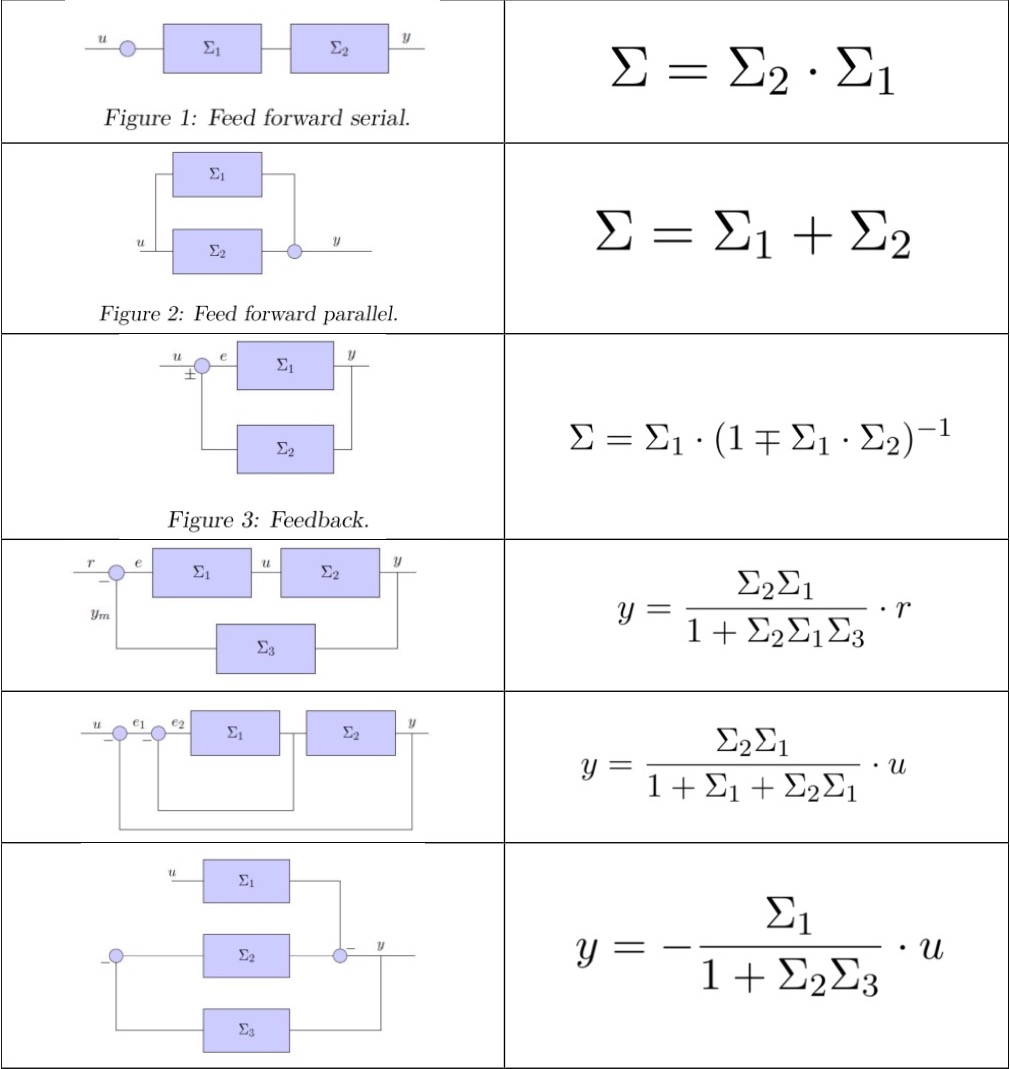
\includegraphics[width=0.75\linewidth]{01/01_signalfluesse.jpg}
            \end{center}


\section{Modellierung}
    Um Differentialgleichungen eines Systems herzuleiten:
    \subsection{Arten der Modellierung}
        \subsubsection{Impulserhaltung}
            \[\frac{d}{dt}(m\dot{x}) = \Sigma_i F_i\]
        \subsubsection{Drehimpulserhaltung}
             \[\frac{d}{dt}(J_B\dot{\theta})= \Sigma_i T_i\]
        \subsubsection{Speichermethode}
          \[\frac{d}{dt}(\textrm{Speicherinhalt}) = \sum \textrm{Zuflüsse} - \sum \textrm{Abflüsse}\]
		\subsubsection{Vorgehen}
		    \begin{enumerate}
    		       
    		    \item  Identifiziere die Systemgrenze (Zuflüsse, Abflüsse)
    
    		    \item  Identifizieren die relevanten Speicher im System (Masse, Energie, Ladung) 
    
    		    \item  Formuliere die DGL
    
     			    $\frac{d}{dt}(\textrm{Speicherinhalt}) = \sum \textrm{Zuflüsse} - \sum \textrm{Abflüsse}$
    
    	    	\item  Formuliere algebraische Relationen der Zuflüsse/Abflüsse eines Speichers als Funktion der Pegelvariablen. %Nach einsetzten sollten sowohl der Speicherinhalt wie auch 				die Zuflüsse/Ausflüsse als Funktion der Pegelvariablen ausgedrückt sein. 
    
    	    	\item  Identifizieren Systemparameter durch Experimente, Designspezifikationen oder Systemoptimiereung
    
    	    	\item  Validiere das Modell mit Experiment
		    \end{enumerate}

    \subsection{Zustandsgleichung}
	    von nicht-linearer DGL in eine Zustandsgleichung erster Ordnung. 
 	    \[\vec{z} = \begin{bmatrix} z \\ z' \\ z'' \\ \vdots \\z^{n-1} \end{bmatrix}  = \begin{bmatrix} z_1 \\ z_2 \\ z_3 \\ \vdots \\z_n \end{bmatrix}
         \xrightarrow{\frac{d}{dt}} \vec{\dot{z}} = \begin{bmatrix} z' \\ z'' \\ z''' \\ \vdots \\z^{n} \end{bmatrix} = \begin{bmatrix} f_1 \\ f_2 \\ f_3 \\ \vdots \\q(z_n,\hdots,z_2,z_1,v) \end{bmatrix}\]
         
    \subsection{Normierung}
        Die Grössen im Zustandsvektor $\vec{z}$ weisen verschiedene Einheiten auf in verschiedenen Größenordnungen. Durch Normierung erhalten wir eine vereinfachte Interpretation und beugen numerische Probleme vor. 
        \[z_i(t) = z_{i,0}\cdot x_i(t), \quad z_{i,0} \in\mathbb{R}\setminus\{0\} \] 
        \textbf{in Vektornotation:}
        \[ z = T \cdot x, \hspace{5mm}  T = \textrm{diag}(z_{1,0},\hdots,z_{n,0})\] 
        \[\Rightarrow x=T^{-1}z\]
    
        Die Ein- und Ausgangsgrössen werden analog normiert:
        \[v(t) = v_0 \cdot u(t) \hspace{5mm} v_0 \in\mathbb{R}\setminus\{0\}\]
        \[w(t) = w_0 \cdot y(t) \hspace{5mm} w_0 \in\mathbb{R}\setminus\{0\}\]
    
        Generell gilt
        \[T \cdot \dot{x} = \dot{z} = f(z,v) \]
        \[w_0 \cdot y = w = g(z,v)\]

\vfill\null\columnbreak
        Nun normiert man das System:
    
        \[ \dot{x} = T^{-1} \cdot f(T \cdot x, v_0 \cdot u) = f_0(x,u) \]
        \[ y = w_0^{-1} \cdot g(T \cdot x, v_0 \cdot u) = g_0(x,u)\]
   
        Die normierte Gleichung $\dot{x} = T^{-1} \cdot f(T \cdot x, v_0 \cdot u) = f_0(x,u)$ hat Einheit: $[\frac{1}{s}]$.
    
    \subsection{Linearisierung}
    
    Nach Normierung wird das System um den Gleichgewichtspunkt linearisiert. 
    
    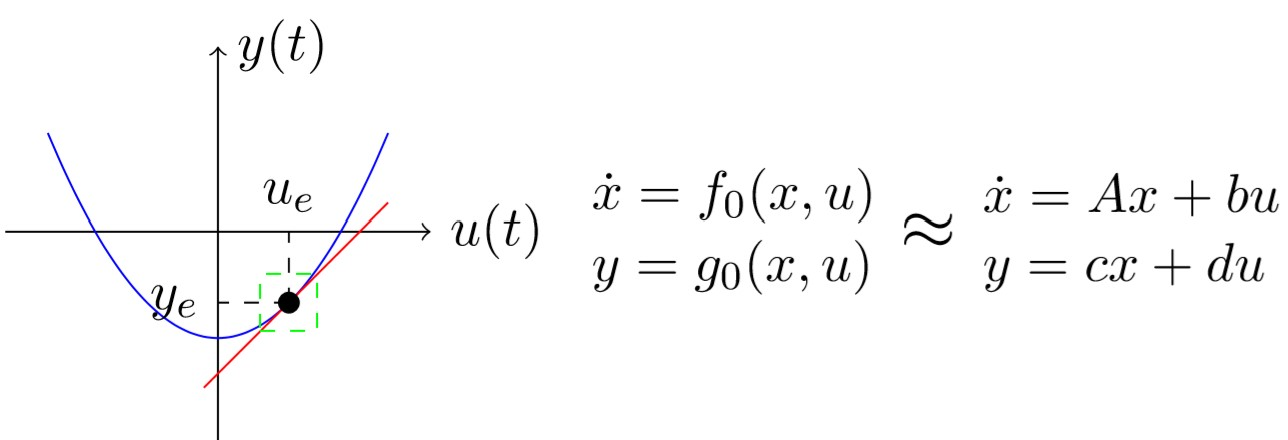
\includegraphics[width=\linewidth, height=30mm]{images/01/01_linearisierung.jpg}
    Um das System zu linearisieren wird zuerst die Gleichgewichtslage berechnet. Im Gleichgewichtszustand gilt per Definition:
    \[ \dot{x} = \begin{bmatrix} \dot{x}_1 \\ \vdots \\ \dot{x}_n\end{bmatrix} = \begin{bmatrix} 0 \\ \vdots \\ 0 \end{bmatrix} = f(x_e,u_e)\]
    
    Dies ist ein lineares Gleichungssystem in $x_1,x_2,...,x_n$ und $u$. Für einen gewünschten Zustand $x_e$ lässt sich ein $u_e$ berechnen. Dabei ist zu beachten, dass nicht alle gewünschten $x_e$ möglich sind. Umgekehrt lässt sich für ein konstantes $u_e$ der resultierende Gleichgewichtszustand $x_e$ berechnen.
    
    Um das System um den Gleichgewichtspunkt zu linearisieren, werden die Matrizen A,b,c,d berechnet:
    
    \begin{center}
        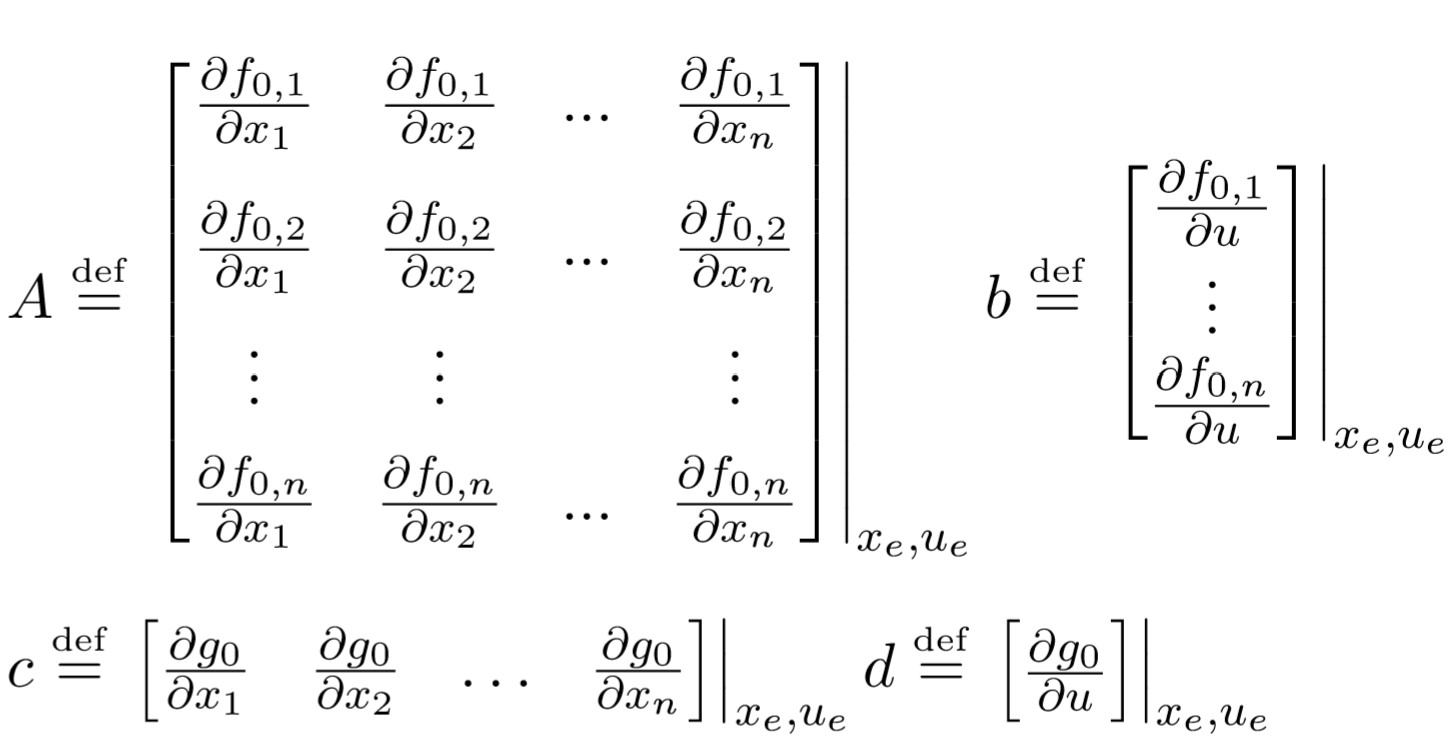
\includegraphics[width=\linewidth]{images/01/01_Statespace.jpg}
    \end{center}
    
    \subsection{Entlinearisierung}
        \begin{center}
            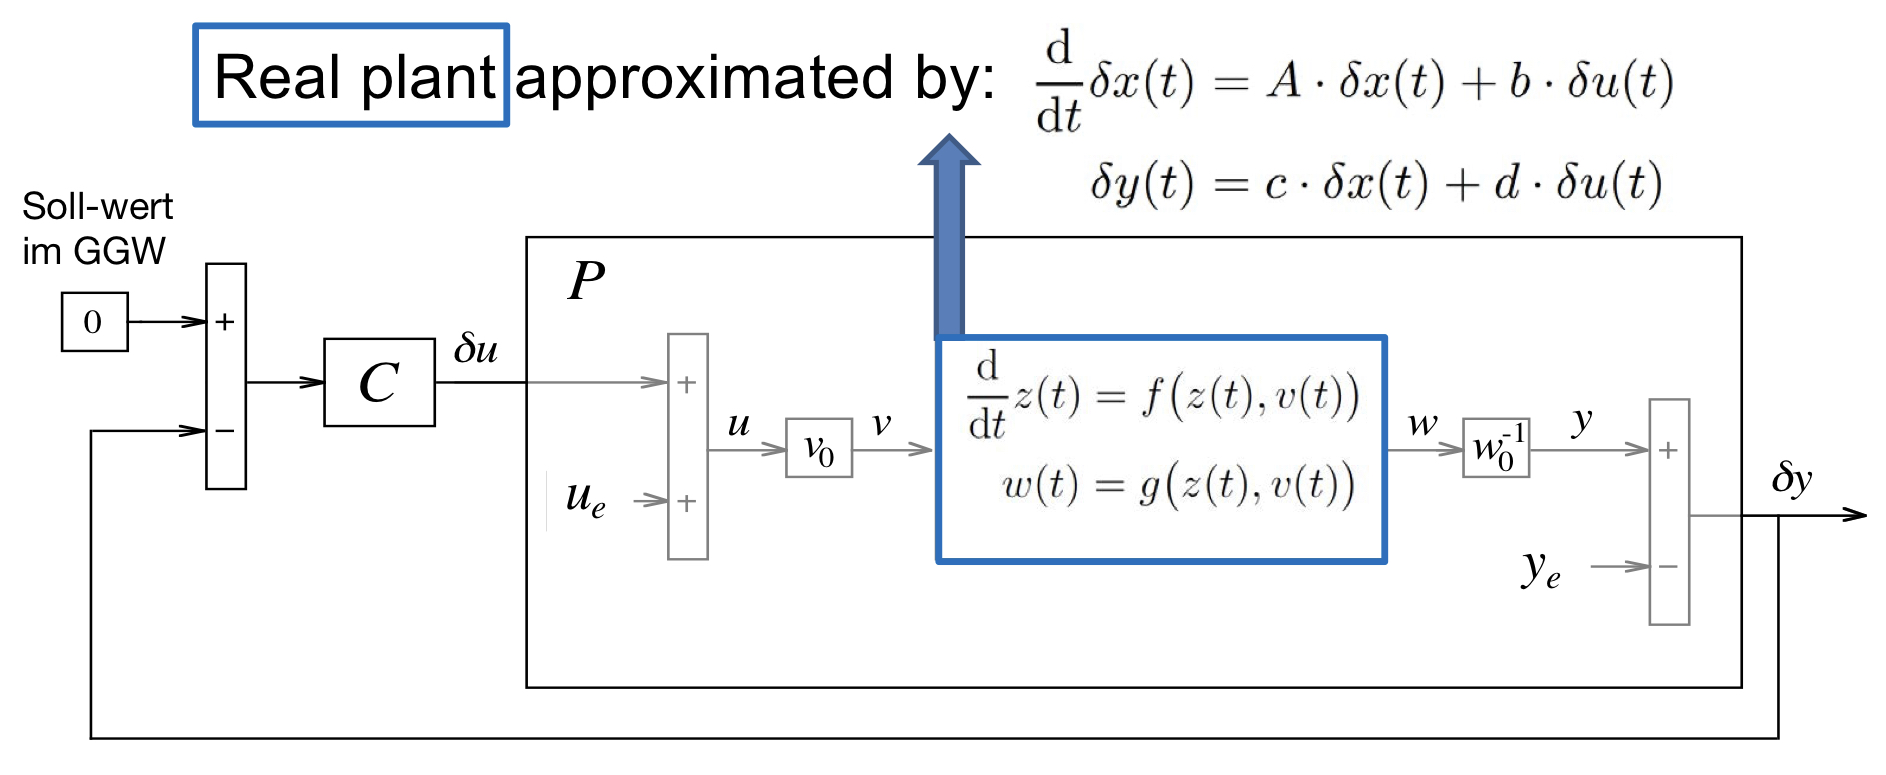
\includegraphics[width=0.8\linewidth]{02/entlinearisierung.jpg}
        \end{center}
    
    \subsubsection{Bsp}
        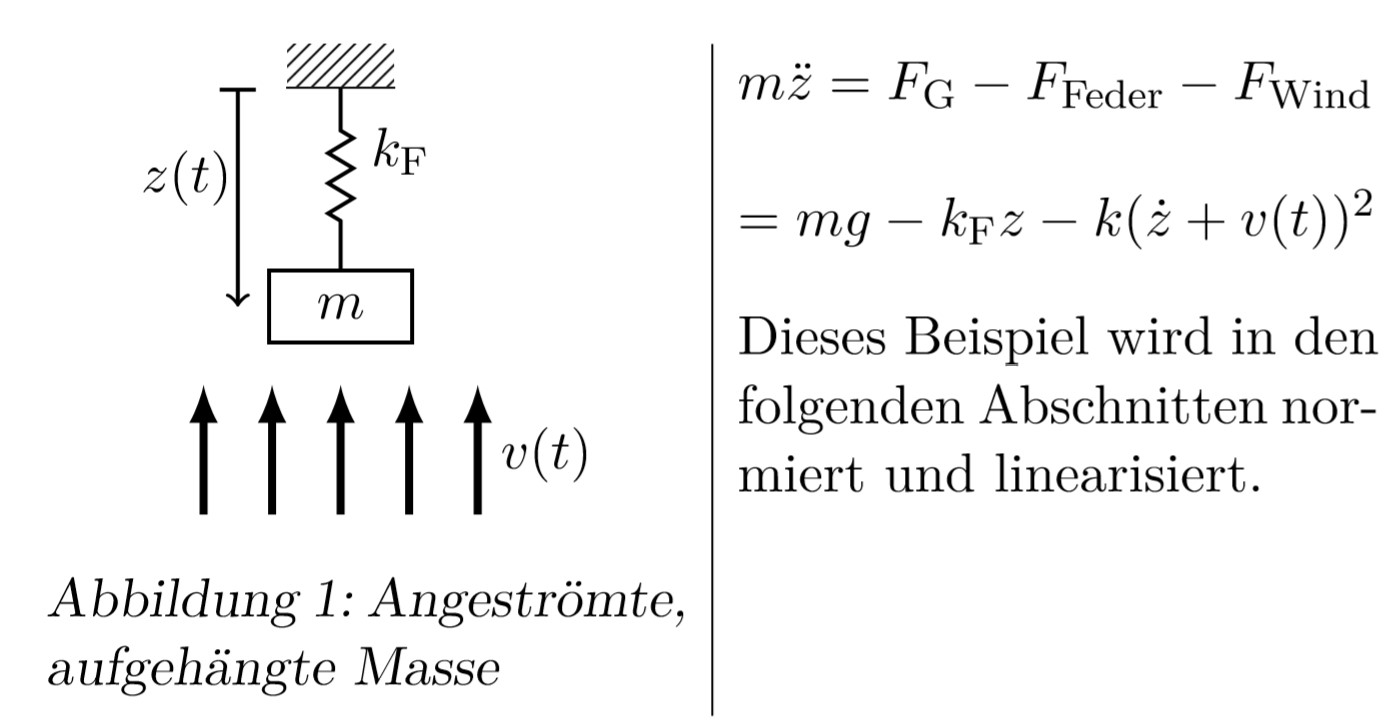
\includegraphics[width=\linewidth,     height=45mm]{images/01/01_bsp.jpg}
        \vspace{-6mm}
        
        \textbf{\underline{Zustandsgleichung:}}
            \[\frac{1}{m}(mg-k_\textrm{F}z-k(\dot{z}+v(t))^2 = \ddot{z}\]
	        \[\vec{z} = \begin{bmatrix} z\\ \dot{z} \end{bmatrix} = \begin{bmatrix} z_1\\ z_2 \end{bmatrix}\]
	        
	        \[\dot{z} = \begin{bmatrix} \dot{z}_1 \\ \dot{z}_2 \end{bmatrix} = \begin{bmatrix} z_2 \\ \frac{1}{m}(mg-k_\textrm{F}z_1-k(z_2+v(t))^2 \end{bmatrix}\]
        \textbf{\underline{Normierung:}}
            
            Es liegt im Interesse des Betrachters, dass die normierte Position $x_1$ der Masse $m$ im Gleichgewichtszustand $p_e$ (bei Wind $v_e$), $x_{1,e} = 1$ entspreche. Ausserdem weiss der Betrachter, dass gilt: $0 < v(t) < v_{max}$. Dies ist hilfreich, um die Eingangsgrösse in die Region $0 < u(t) < 1$ zu normieren. Die maximale Geschwindigkeit $\dot{z}_{max}$ sei $h$:
            
            \[ T = \begin{bmatrix} p_e & 0 \\ 0 & h \end{bmatrix}, \hspace{5mm} v(t) = v_{max} \cdot u(t)\]
            \[\dot{x} = \begin{bmatrix} \frac{h}{p_e}\cdot x_2 \\ \frac{1}{h \cdot m}(mg-k_\textrm{F} \cdot p_e \cdot x_1 - k(h\cdot x_2+v_{max} \cdot u(t))^2)\end{bmatrix} \]
            
        \textbf{\underline{Linearisierung:}}
            
            \[\dot{x}_e = \begin{bmatrix}\frac{h}{p_e}\cdot x_{2,e} \\ \frac{1}{h \cdot m}(mg-k_\textrm{F} \cdot p_e \cdot x_{1,e} - k(h\cdot x_{2,e}+v_{max} \cdot u_e)^2)\end{bmatrix} \]	
            \[= \begin{bmatrix} 0 \\ 0\end{bmatrix} \Rightarrow x_{2,e} = 0, \hspace{3mm} u_e = \frac{1}{v_{max}}\sqrt{\frac{1}{k}(mg-k_\textrm{F}p_e\cdot x_{1,e}}), \]
            
            mit $x_{1,e}=1$.
            	
            Um das System um den Gleichgewichtspunkt zu linearisieren, werden die Matrizen A,b,c,d berechnet:
            \[A = \begin{bmatrix} 0 & \frac{h}{p_e} \\ -\frac{1}{h \cdot m} \cdot k_\textrm{F} \cdot p_e & -\frac{1}{m}\cdot 2k \cdot(h\cdot x_{2,e} + v_{max} \cdot u_e) \end{bmatrix},\]
            
            \[ b = \begin{bmatrix} 0 \\ -\frac{1}{h\cdot m} \cdot 2k \cdot v_{max} \cdot (h\cdot x_{2,e} + v_{max} \cdot u_e) \end{bmatrix}\]
             
             \[ c = \begin{bmatrix} 1 & 0 \end{bmatrix}; \quad d = 0\]

    \subsubsection{Bsp}
            \[\begin{cases}
            \dot{x}_1=x_2\\
            \dot{x}_2=-2x_1-3x_2+10u\\
            y= x_1
            \end{cases}
            \]
        \[\Downarrow{Simulink-Modell}\]
        \begin{center}
            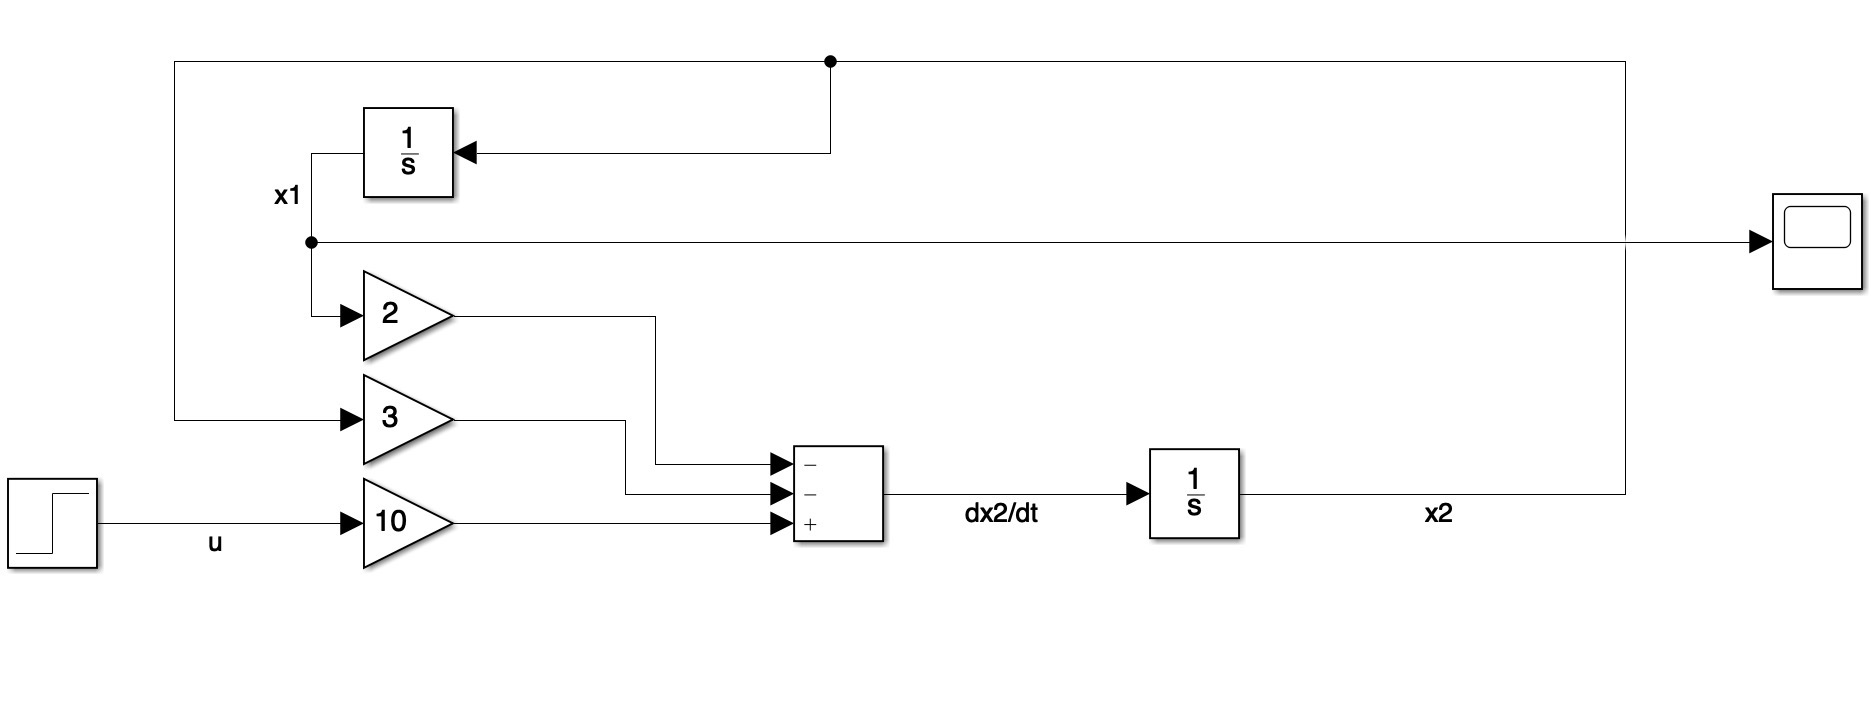
\includegraphics[width=0.8\linewidth]{images/02/simulink.jpeg}
        \end{center}
        \[\Downarrow{State\textrm{-}Space\textrm{ }Matrizen}\]
        \[A= \begin{bmatrix}
            0 & 1 \\ -2 & -3
        \end{bmatrix};\quad b=
        \begin{bmatrix}
        0\\10
        \end{bmatrix}
        \]
        \[c=\begin{bmatrix}
        1 & 0
        \end{bmatrix};\quad d=0\]
        
        
\vfill\null\columnbreak
\section{Systemanalyse im Zeitbereich}
Für ein lineares zeitinvariantes SISO System gilt:
    \subsection{Allgemeine Lösung}
        \[ \dot{x}(t) = A \cdot x(t) + b \cdot u(t) \hspace{4mm} A \in\mathbb{R}^{n \times n}, b \in\mathbb{R}^{n \times 1} \]
        \[ y(t) = c \cdot x(t) + d \cdot u(t) \hspace{4mm} c \in\mathbb{R}^{1 \times n}, d \in\mathbb{R}\]
        \[x(0) = x_0\]
        
        die allgemeine Lösung der Zustandsgrösse $x(t)$ ist gegeben als: 
        \[ x(t) = e^{A\cdot t} \cdot x_0 + \int_0^t e^{A\cdot(t-p)}\cdot b \cdot u(p)dp\]
        
        Setzt man die allgemeine Lösung in die Gleichung der Ausgangsgrösse y(t) ein, erhält man die Superposition dreier Grössen:
        
         \[ y(t) = \underbrace{c\cdot e^{A\cdot t} \cdot x_0}_\text{I} + c \underbrace{\cdot \int_0^t e^{A\cdot(t-p)}\cdot b \cdot u(p)dp}_\text{II} + \underbrace{d\cdot u(t)}_\text{III}\]
         
         Die \textbf{natürliche Antwort} des Systems ($I$) ist unabhängig von der Eingangsgrösse $u$. Der Eingang u trägt einerseits zum Beitrag der \textbf{Systemdynamik} ($II$) bei, und andererseits zum \textbf{Feedthrough Term} ($III$)
    \subsection{Stabilitätseigenschaften}
        Um die Stabilität eines Systems zu bestimmen betrachtet man die natürliche Antwort des Systems ($u(t)=0$). Da die Zustandsgleichungen im Allgemeinen gekoppelt sind führt man eine Koordinatentransformation durch.
        \[\Tilde{x}=V^{-1}\cdot e^{A\cdot t}\cdot V \cdot\Tilde{x}(0)=e^{\Tilde{A}\cdot t}\cdot\Tilde{x}(0)\]
        \[\Tilde{x}=
        \begin{bmatrix}
            e^{\lambda_1\cdot t}    & 0                     & \dots & 0 \\
            0                       & e^{\lambda_2\cdot t}  & \dots & 0 \\
            \vdots                  & \ddots                & \ddots & \vdots\\
            0                       & \dots    &\dots             & e^{\lambda_n\cdot t}
        \end{bmatrix}
        \Tilde{x_0}=
        \begin{bmatrix}
            e^{\lambda_1\cdot t}\cdot\Tilde{x}_{0,1}  \\
            e^{\lambda_2\cdot t}\cdot\Tilde{x}_{0,2} \\
            \vdots  \\
            e^{\lambda_n\cdot t}\cdot\Tilde{x}_{0,n} 
        \end{bmatrix}
        \]
        wobei $\lambda_i$ die Eigenwerte von $A$ (resp. $a^{-1}$) sind. Da die EW generell Komplex sind ($\lambda_i=\sigma_i+j\omega_i$) kann man die obige Gleichung auch umschreiben.
        \[
        \begin{bmatrix}
            e^{\lambda_1\cdot t}\cdot\Tilde{x}_{0,1}  \\
            e^{\lambda_2\cdot t}\cdot\Tilde{x}_{0,2} \\
            \vdots  \\
            e^{\lambda_n\cdot t}\cdot\Tilde{x}_{0,n} 
        \end{bmatrix}
        =
        \begin{bmatrix}
            e^{\sigma_1\cdot t}\cdot\left(cos(\omega_1t)+j\cdot sin(\omega_1t)\right)\cdot\Tilde{x}_{0,1}  \\
            e^{\sigma_2\cdot t}\cdot\left(cos(\omega_2t)+j\cdot sin(\omega_2t)\right)\cdot\Tilde{x}_{0,2} \\
            \vdots  \\
            e^{\sigma_n\cdot t}\cdot\left(cos(\omega_nt)+j\cdot sin(\omega_nt)\right)\cdot\Tilde{x}_{0,n} 
        \end{bmatrix}
        \]
        \begin{center}
            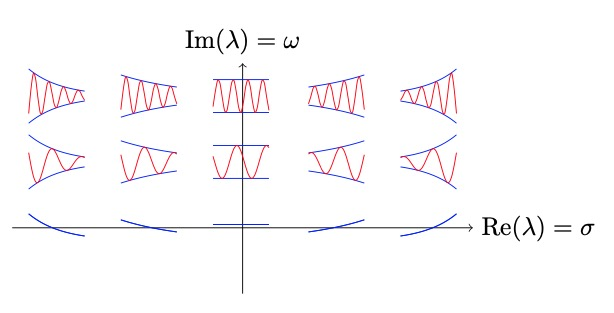
\includegraphics[width=0.8\linewidth]{03/sysantwort.jpg}
            %Symmetrisch um $\textrm{Re}(\lambda)=\sigma$-Achse.
        \end{center}
        
    \subsection{Lyapunov Stabilität}
        Stabilität nach Lyapunov erlaubt die Stabilitätsanalyse von Gleichgewichstpunkten (GGWP) von linearen und linearisierten Systemen.\\\\
        \textbf{WICHTIG! Falls ein GGWP eines linearisierten Systems Eigenwerte mit $\sigma_i=0$ hat, lässt sich keine Aussage über die Stabilität dieses GGWP des nichtlinearen Systems machen.}
        \begin{enumerate}
            \item \textbf{Asymptotisch stabil:} $\displaystyle\lim_{t\to\infty}\Vert x(t)\Vert = 0 $, falls alle EW $\textrm{Re}(\lambda_i)<0$.
            \item \textbf{Stabil:} ($\Vert x(t)\Vert<\infty \forall t \in[0,\infty]$), falls mehrere EW $\textrm{Re}(\lambda_k)=0$ und kein EW $\textrm{Re}(\lambda_i)\ngtr 0$.
            \item \textbf{Instabil:} $\displaystyle\lim_{t\to\infty}\Vert x(t)\Vert = \infty$ falls mindestens ein EW $\textrm{Re}(\lambda_i)>0$.
        \end{enumerate}{}
        \subsubsection{Bsp}
            \[m\Ddot{x}=-c_D\dot{x}-k_Fx+u(t)\]
            \[\Rightarrow \Ddot{x}=
                \begin{bmatrix}
                    0   &   1\\
                    -k_F/m  &   -c_D/m\\
                \end{bmatrix}
                \begin{bmatrix}
                    x_1\\
                    x_2\\
                \end{bmatrix}
                +
                \begin{bmatrix}
                0\\
                1\\
                \end{bmatrix}
                u(t)
            \]
            \[\textrm{Det}(A-\lambda\mathbb{I}) \Rightarrow \lambda_i=-\frac{c_D}{2m}\pm \sqrt{\frac{c_D^2}{4m^2}-\frac{k_F}{m}}\]
            
            \begin{enumerate}
                \item $\displaystyle \frac{c_D^2}{4m^2}-\frac{k_F}{m}\geqslant 0
                \Leftrightarrow c_D^2 \geqslant 4k_Fm \Rightarrow\boxed{\sigma_i<0,\omega_i=0}$
                
                Falls der Dämpfer relativ zur Feder und zur Masse genug stark ist, sind alle EW reellwertig negativ. Dh, das System konvergiert ohne Oszillation zum GGWP. \boxed{\textrm{\textit{Asymptotisch stabil} nach Lyapunov.}}
                \item $\displaystyle c_D^2 \leqslant 4k_Fm \Rightarrow\boxed{\sigma_i<0,\omega_i\neq0}$
                \\Falls der Dämpfer schwach ist, werden die EW komplex, mit negativem Realteil. Dh, das System oszilliert um den GGWP mit abnehmender Amplitude. \boxed{\textrm{\textit{Asymptotisch stabil} nach Lyapunov.}}
                \item $\displaystyle c_D=0 \Rightarrow\boxed{\sigma_i=0,\omega_i\neq0}$
                \\Falls kein Dämpfer im System vorhanden ist, werden alle Eigenwerte Komplex mit Realteil $\sigma_i=0$. Das System oszilliert für immer um den GGWP.
                \boxed{\textrm{\textit{Stabil} nach Lyapunov.}}
                \item $\displaystyle k_F=0 \Rightarrow\boxed{\lambda_1=0,\sigma_2<0,\omega_2=0}$
                \\Falls keine Feder im System ist, wird ein EW 0 und der andere wird reell negativ. Falls das System mehrmals angestossen wird, kommt es jedes mal ohne Oszillation zum Stillstand, jedoch nicht zwingend um den GGWP.
                \boxed{\textrm{\textit{Stabil} nach Lyapunov.}}

                
            \end{enumerate}
        
        \subsection{Testsignale auf Systeme erster Ordnung}
            Eingänge für Systeme erster Ordnung mit Zeitkonstante $\tau$ und Eingangsstärke $k$:
            \[\dot{x}(t) = -\frac{1}{\tau}x(t) + \frac{k}{\tau}u(t), \hspace{5mm} y(t) = x(t)\]
            \subsubsection{Impulsantwort}
                \[u(t) = \delta(t) = \begin{cases} +\infty, & t = 0, \\ 
                0, & t \neq 0 \end{cases}\]
                \textbf{Allgemeine Lösung:}
                \[y_{\delta}(t) = e^{\frac{-t}{\tau}}\cdot(x_0+\frac{k}{\tau})\]
        
                Ein Impuls ändert die Anfangsbedingung $x_0$ um $k / \tau $.
        
                $\rightarrow$ Impuls induziert eine Anfangsbedingung, System entwickelt sich von der neuen Anfangsbedingung, als ob $u(t) = 0$ wäre.
    
            \subsubsection{Sprungantwort}
%               \[ u(t) = h(t) = \begin{cases}
%               1, & t \geq 0\\
%               0, & t <0 \end{cases}\]
                \textbf{Allgemeine Lösung:}
                \[y_h(t) = e^{\frac{-t}{\tau}}\cdot x_0 + k \cdot (1-e^{\frac{-t}{\tau}}) \]
                \begin{center}
                    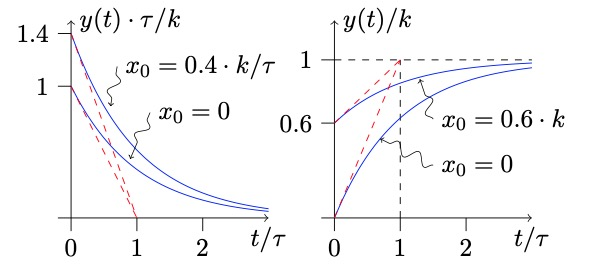
\includegraphics[width=0.7\linewidth]{03/impuls-Sprung-Antwort.jpg}\\
                    \textit{Impulsantwort links und Sprungantwort rechts.}
                \end{center}
                Die Tangente an die Impulsantwort zum Zeitpunkt $t=0$ schneidet die Zeitachse zum Zeitpunkt $t=\tau$. 
                \\Die Tangente an die Sprungantwort schneidet den Sprung $k\cdot h(t)$ auch zum Zeitpunkt $t=\tau$.
                \\Impulsantwort hat bei $t=0$ den Wert $\frac{k}{\tau}$.
                \\$\Rightarrow$ \textbf{Je kleiner $\mathbf{\tau}$, desto schneller konvergiert das System.}
            \subsubsection{Rampenantwort}
%               \[u(t)=p(t)=\begin{cases}
%               t, & t \geq 0\\
%               0, & t < 0 \end{cases}\]
                \textbf{Allgemeine Lösung:}
                \[y_p(t)=e^{-\frac{t}{\tau}}x_0+k(t+(e^{-\frac{t}{\tau}}-1)\tau)\]
            \subsubsection{Bsp}
                $\dot{x}(t)=-\frac{c_D}{m}x(t)+\frac{1}{m}u(t)\qquad\Rightarrow \tau = \frac{m}{c_D};\qquad k=\frac{\tau}{m}=\frac{1}{c_D}$
                \begin{center}
                    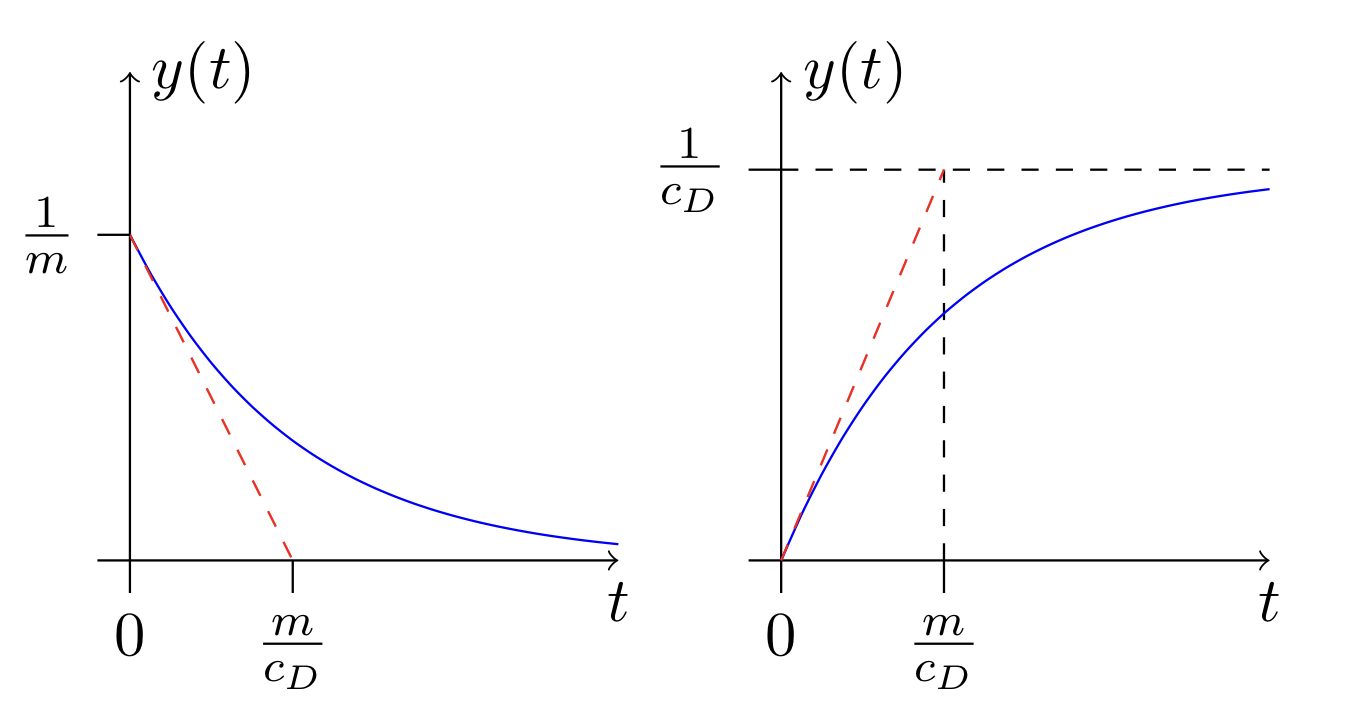
\includegraphics[width=0.75\linewidth,]{03/bsp_impuls_sprung.jpeg}
                \end{center}
                
        \subsection{Steuerbarkeit / Erreichbarkeit}
            \textbf{Steuerbar}
        falls für $x_c \in\mathbb{R}^n$ ein Eingangssignal $u(t)$ existiert, das den Zustandsvektor des Systems von $x(0) = x_c $ zum Zustand $x(\tau) = 0$ (zum Ursprung) in endlicher Zeit $\tau$ bringt. 
        
        Falls alle Punkte in $\mathbb{R}^n$ steuerbar sind, heisst das System \textit{ vollständig steuerbar}.
        Falls alle nicht-steuerbaren Zustände asymptotisch stabil sind, ist das System \textit{potentiell stabilisierbar}, 
        
        \textbf{Erreichbar} falls für $x_r \in\mathbb{R}^n$ ein Eingangssignal $u(t)$ existiert, das den Zustandsvektor des Systems von Zustand $x(t) = 0$ zum Zustand $x(\tau) = x_r$ in endlicher Zeit $\tau$ bringt.
        
        Falls alle Punkte in $\mathbb{R}^n$ erreichbar sind, heisst das System vollständig erreichbar.
        
        \textbf{WICHTIG: Für LZI Systeme sind die Teilräume der erreichbaren und steuerbaren Zustände identisch. }
        
        ein System ist vollständig steuerbar/erreichbar, wenn die \textbf{Steuerbarkeitsmatrix $\mathcal{R}$} vollen Rang hat ($\textrm{Det}(\mathcal{R})\neq0$). 
        \[\mathcal{R} = \begin{bmatrix} b, & A\cdot b, & A^2 \cdot b, & \hdots, & A^{n-1} \cdot b \end{bmatrix} \]
        \textbf{Alle Steuerbaren Zustände sind Linearkombinationen der Spalten von $\mathcal{R}$}
        
        \subsubsection{Bsp}
            \begin{center}
                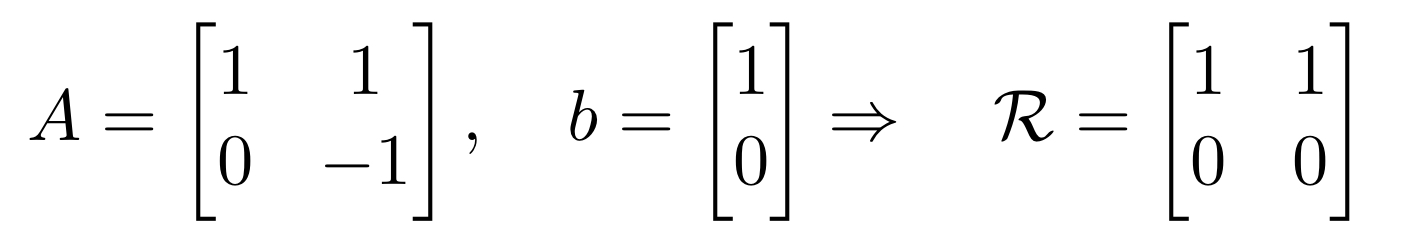
\includegraphics[width=0.7\linewidth]{03/steuerbarkeit.jpeg}\\
                $\displaystyle \textrm{Det}(\mathcal{R})\neq 0 \rightarrow$ Steuerbar
            \end{center}
            
            $\textrm{Rank}(\mathcal{R})=1<n\rightarrow$ System ist nicht vollständig erreichbar. Aus $\{A,b\}$ folgt, dass der zweite Zustand nicht direkt vom Eingang beeinflusst wird.
        \subsubsection{Stabilisierbar}
            Ein (instabiles) System ist potentiell Stabilisierbar, falls alle Zustände, die nicht steuerbar sind asymptotisch stabil sind.
            
            \textit{Remarks:}
            \\Stabilizability is a weaker condition than controllability.
            \\To stabilize an unstable system, the unstable but controllable variables have to be observable as well.
        \subsection{Beobachtbarkeit}
            Ein System ist vollständig beobachtbar, wenn man mit der Messung des Ausgangssignals $y(t), t \in [0,\tau], \tau > 0$ eindeutig auf den Anfangszustand $x(0)$ des Systems schliessen kann. 
            
            Ein LZI System ist dann vollständig beobachtbar, wenn die \textbf{Beobachtbarkeitsmatrix $\mathcal{O}$} vollen Rang hat ($\textrm{Det}(\mathcal{O})\neq0$).
            \[ \mathcal{O} = \begin{bmatrix} c \\ c \cdot A \\ c \cdot A^2 \\ \vdots \\ c \cdot A^{n-1}\end{bmatrix}\]
            
            \subsubsection{Bsp}
            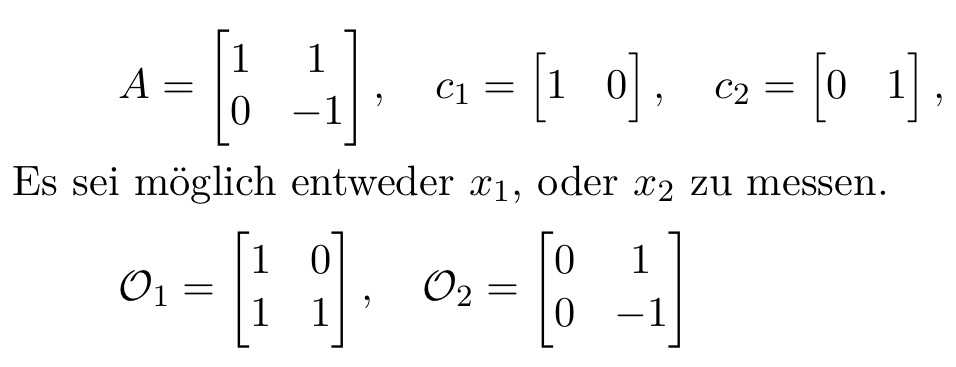
\includegraphics[width=0.8\linewidth]{03/observability.jpeg}
            \\Falls man $x_1$ misst, ist das System \textbf{vollständig beobachtbar}: $\textrm{Rank}(\mathcal{O}_1)=2$ D.h. man kann durch messen von $x_1$ auf die Anfangsbedingungen von $x_1(0)$ \& $x_2(0)$ schliessen. Falls man nur $x_2$ misst, erhält man $\textrm{Rank}(\mathcal{O}_2=1<n$. Das System ist somit nicht vollständig beobachtbar. Das ist auch in der graphischen Darstellung ersichtlich:
            \begin{center}
                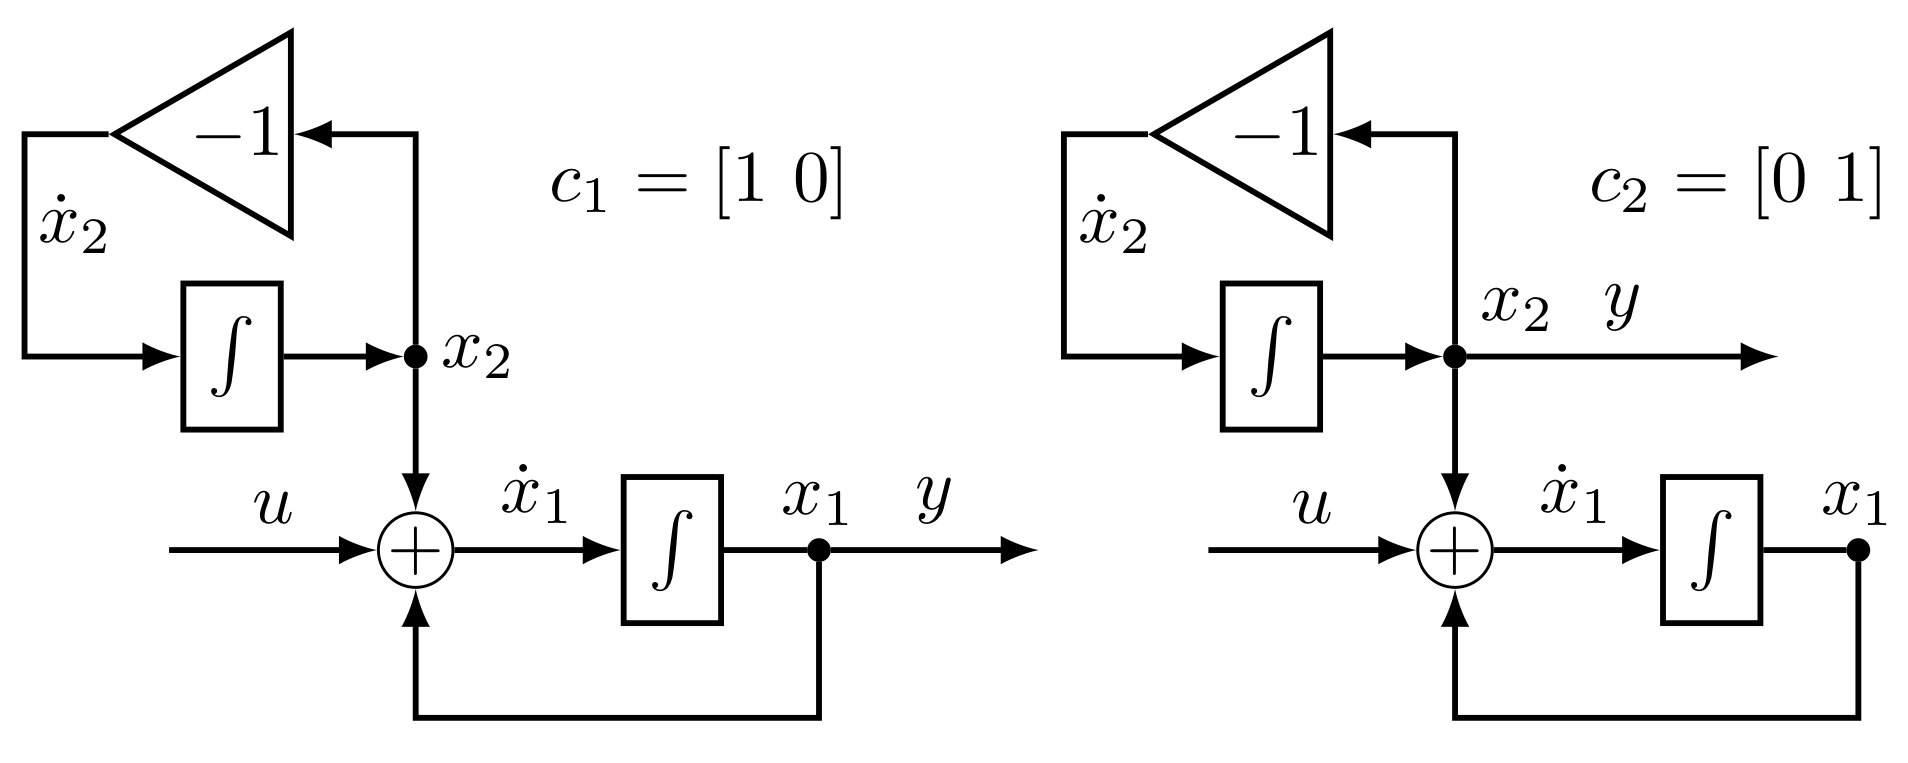
\includegraphics[width=0.6\linewidth]{03/graphisch.jpeg}
            \end{center}
        \subsubsection{Detektierbarkeit}
           Ein System ist nur detektierbar, falls all seine nicht-beobachtbaren Zustände asymptotisch stabil sind.
           
           \textit{Remarks:}
           \\Detectability is a weaker condition than observability.
           \\An (unstable) system is stabilizable, if the system is potentially stabilizable \textit{and} detectable.
            
        \subsection{Koordinatentransformationen} Ein Zustandsraum mit Koordinaten $x$ kann durch eine Koordinatentransformation in anderen Koordinaten $\tilde{x}$ beschrieben werden.
        \[ x(t) = T \cdot \tilde{x}(t) \hspace{10mm} T \in\mathbb{R}^{n\times n}, det(T)\neq0\]
        \[\frac{d}{dt}\tilde{x}(t) = T^{-1} \cdot A\cdot T \cdot \tilde{x}(t) + T^{-1} \cdot b \cdot u(t)\]
        \[y(t) = c\cdot T \cdot \tilde{x}(t) + d \cdot u(t)\]
        
        Fundamentale Systemeigenschaften  (Stabilität, Steuerbarkeit, Beobachtbarkeit, I/O-Verhalten) sind Transformationsinvariant.
\vfill\null\columnbreak        
        \subsection{Input/Output (I/O) Darstellung}
            Eine Zustandsraumdarstellung $\{A,b,c,d\}$ beschreibt das gesamte System (Zustände $x(t)$ und Ausgang $y(t)$ für gegebene $x(0) \& u(t)$). Oftmals ist man aber nur am I/O Zusammenhang $u(t) \rightarrow y(t)$ interessiert.\\\\
            \textbf{I/O-Beschreibung:}
            \begin{center}
                $\displaystyle y^{(n)}(t)+a_{n-1}\cdot y^{(n-1)}(t)+\dots+a_1\cdot y^{(1)}(t)+a_0\cdot y(t) = b_m\cdot u^{(m)}(t)+\dots+b_1\cdot u^{(1)}(t)+b_0\cdot u(t)$
            \end{center}
            
        
        \subsection{Zustandsraum Normalformen}
            Zustandsraumdarstellungen, welche sich für Analyse-Methoden besonders eignen, sind Normalformen oder eine kanonische Form.
            
            Eine wichtige Normalform ist die \textbf{Reglernormalform}.
            \begin{center}
               \[\left[{\renewcommand{\arraystretch}{1.3}\begin{array}{c|c}
              A & b\\
            \hline
            c & d
            \end{array}}
               \right]= \left[{\renewcommand{\arraystretch}{1.4}\begin{array}{ccccc|c}
               0 & 1 & 0 & \cdots & 0 & 0 \\
               0 & 0 & 1 &\ddots & \vdots & \vdots\\
            \cdots & \cdots & \cdots & \ddots & \vdots & \vdots \\
            0 & 0 & 0 & \cdots & 1 & 0\\
            -a_0 & -a_1 & -a_2 & \cdots & -a_{n-1} & 1 \\
            \hline
            b_0 & \cdots & b_m & 0 & \cdots & d
               \end{array}}
             \right]
               \] 
            \end{center}
            wobei $a_i,b_j$ aus der I/O-Darstellung oder aus $\Sigma(s)$ kommen:
            \[\Sigma(s) =\frac{b_ms^m+\dots+b_3s^3+b_2s^2+b_1s+b_0}{s^n+a_{n-1}s^{n-1}+\dots+a_3s^3+a_2s^2+a_1s+a_0}+d\]
        \subsection{Zustandsraumzerlegung}
            Die Sets von erreichbaren ($\mathcal{R}$) und/oder beobachtbaren ($\mathcal{O}$) Punkten sind \textbf{invariante Unterräume} im Zustandsraum. durch eine geeignete Koordinatentransformation $x = T\cdot\tilde{x}$ kann der gesamte Zustandsraum in die invarianten Unterräume $\{\tilde{x}_1,\tilde{x}_2,\tilde{x}_3,\tilde{x}_4\}$ zerlegt werden:
            Für die Beschreibung des I/O-Verhaltens ist also nur der Zustand $\tilde{x}_3$ relevant, da er der einzige ist, der gleichzeitig beobachtbar UND steuerbar ist. Die Anzahl Zustände $n$ im Unterraum $\tilde{x}_3$ entspricht der minimalen Anzahl Zustände, die zur Beschreibung des I/O-Verhaltens nötig sind. Deshalb wird die Darstellung des Systems in den Koordinaten $\tilde{x}_3$ \textbf{minimale Zustandsraumdarstellung} genannt:
            \begin{center}
                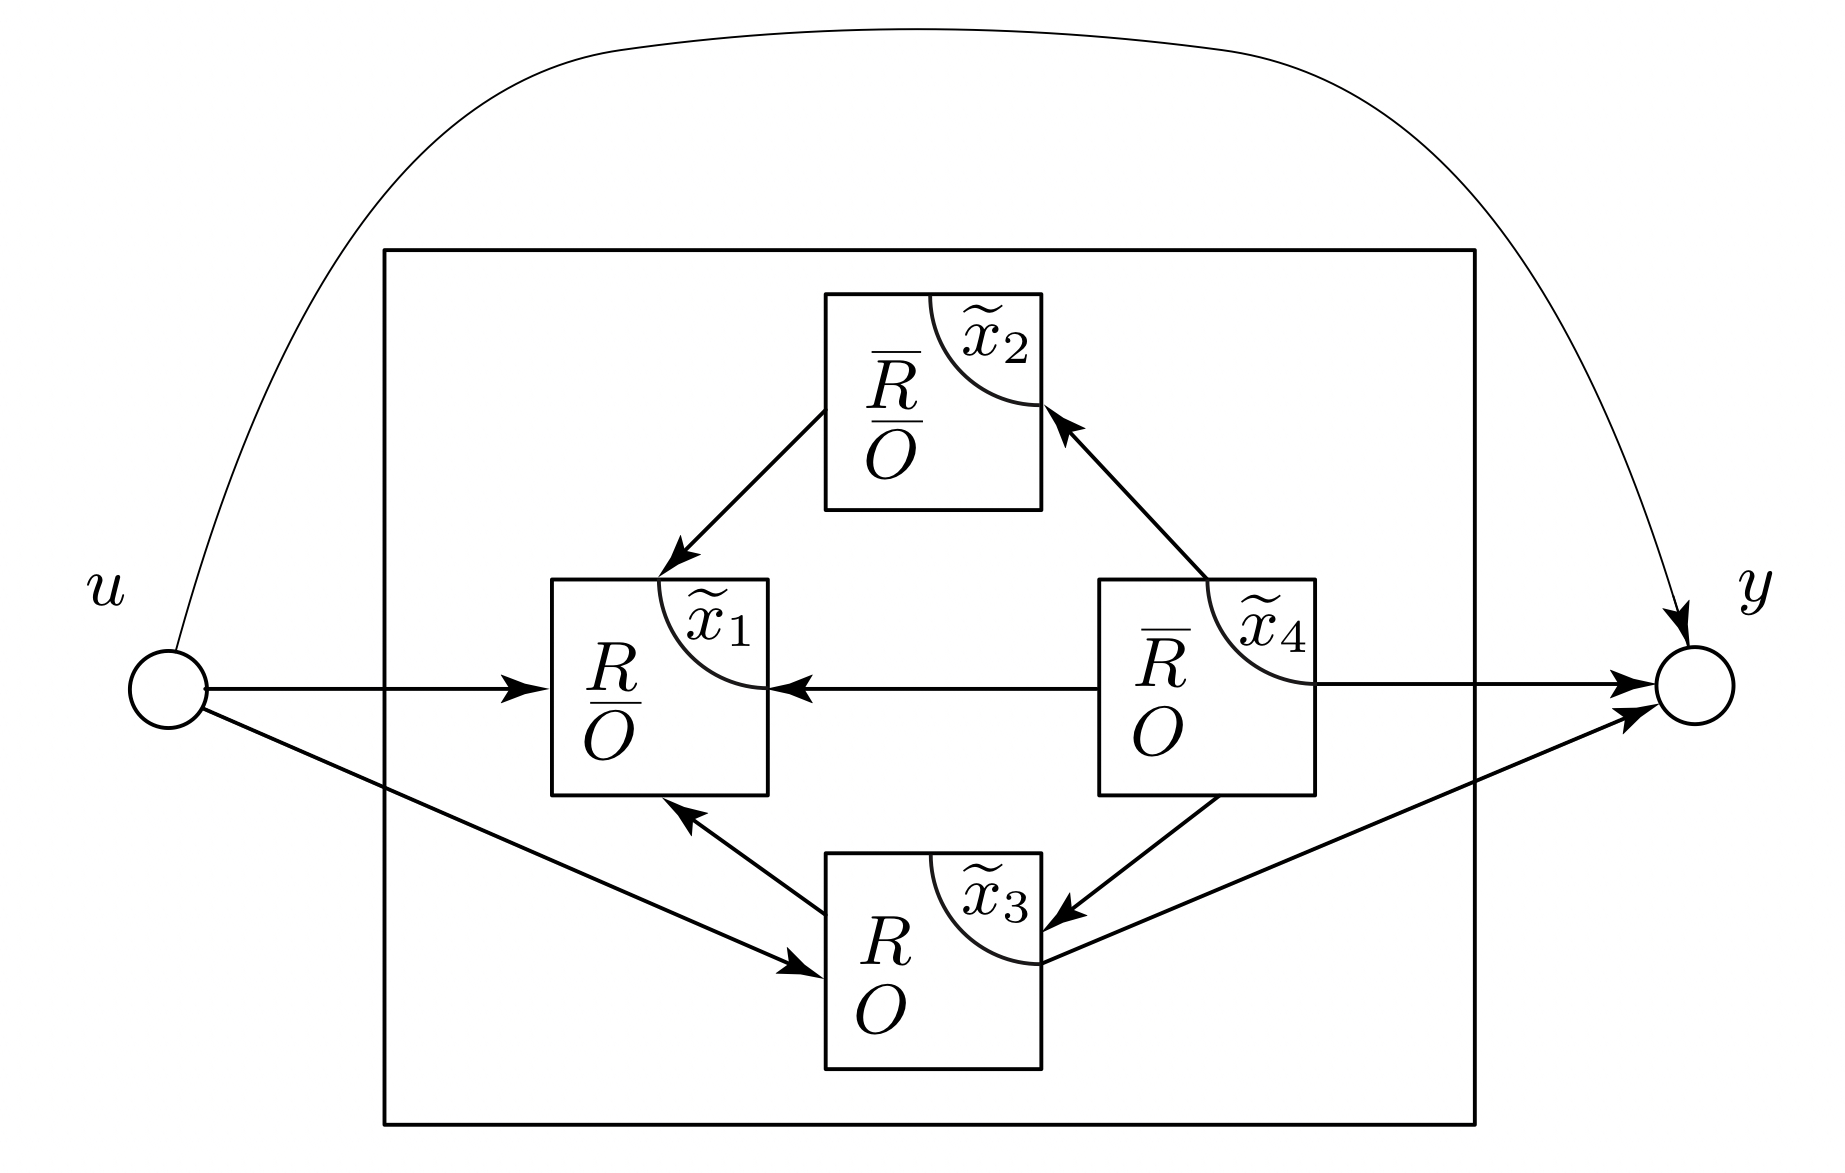
\includegraphics[width=0.4\linewidth]{03/invarianten.jpeg}
                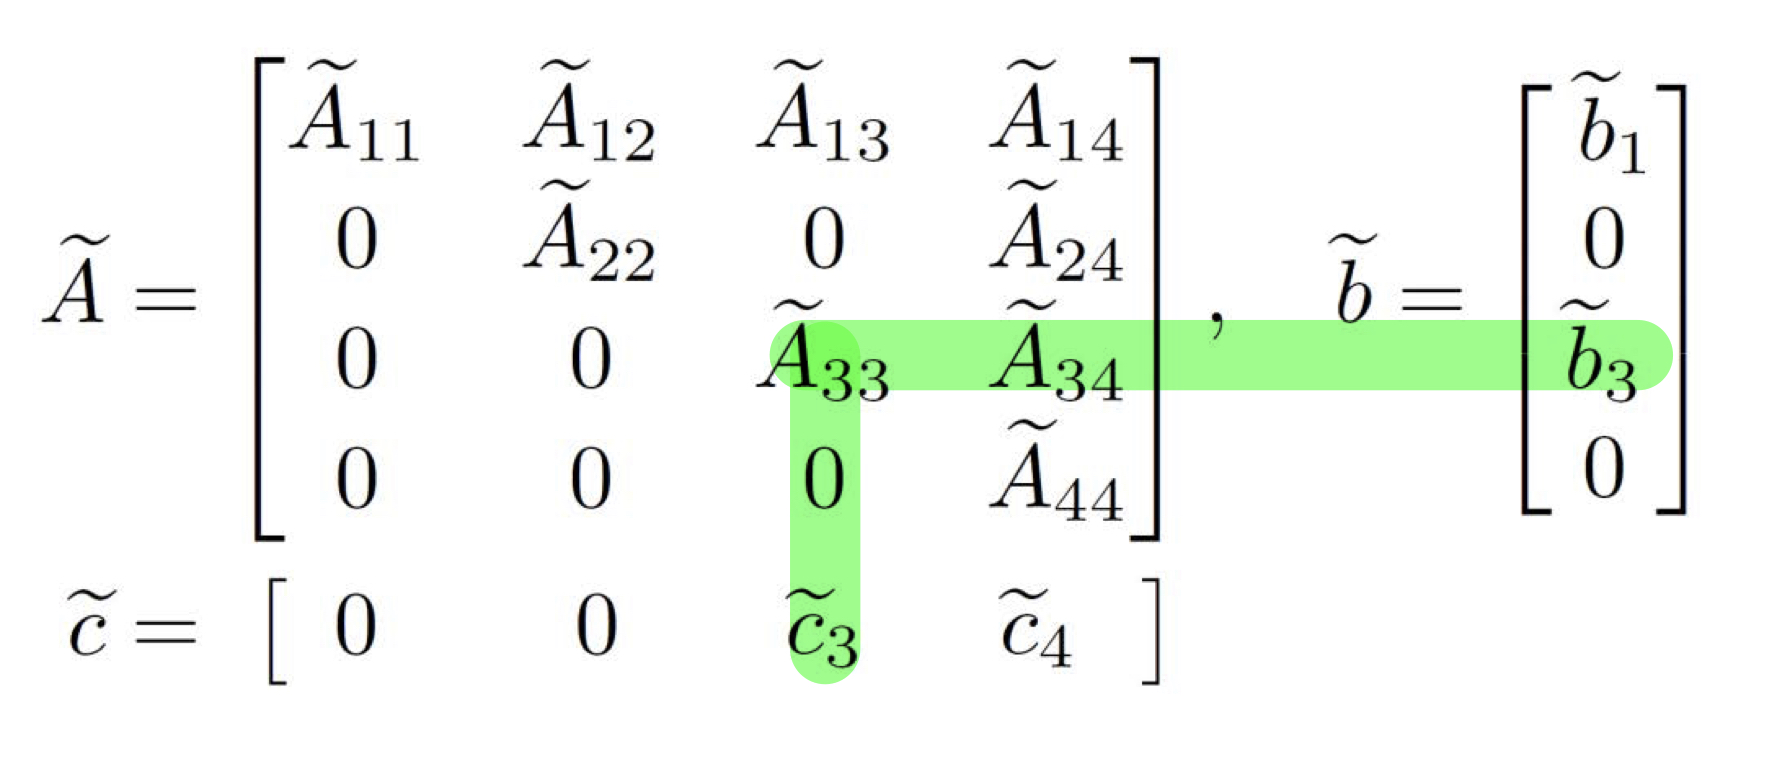
\includegraphics[width=0.5\linewidth]{03/minimal.jpeg}
                \\minimal realization $\rightarrow\{\tilde{A}_{33},\tilde{b}_3,\tilde{c}_3,d\}$ 
            \end{center}
            Vollständig steuerbar und beobachtbar (falls keine Pol-NST-Kürzung möglich, ist das System bereits in minimaler Form).
            % direkt Aus Systemmatrizen auslesen oder in Übertragungsfunktionsform $\Sigma(s)$ bringen und in Reglernormalform rücktransformieren. 
            
        \subsubsection{Bsp}
            Bestimme ob $\{A,b\}$ steuerbar ist, ohne $\mathcal{R}$ zu berechnen.
            \[ A=
            \begin{bmatrix}
            -1  &   -2  &   0\\
            -2  &  -1  &   0\\
            0   &   0   &   -2\\
            \end{bmatrix},
            b=
            \begin{bmatrix}
            1\\ 1\\ 1\\
            \end{bmatrix}
            \]
            \[\Downarrow diagonalisieren\quad \dot{\Tilde{x}}=D\cdot\Tilde{x}+V^{-1}\cdot b\cdot u\]
            \[
            \begin{bmatrix}
                \dot{\Tilde{x}}_1\\
                \dot{\Tilde{x}}_2\\
                \dot{\Tilde{x}}_3\\
            \end{bmatrix}
            =
            \begin{bmatrix}
            -3  &   0   &   0\\
            0   &   -2  &   0\\
            0   &   0   &   1\\
            \end{bmatrix}
            \cdot
            \begin{bmatrix}
                \Tilde{x}_1\\
                \Tilde{x}_2\\
                \Tilde{x}_3\\
            \end{bmatrix}
            +
            \begin{bmatrix}
            \sqrt{2}\\
            1\\
            0\\
            \end{bmatrix}
            \cdot
            u
            \]
            %$D$: Matrix mit diag($\lambda_i$) \& $V$ Matrix mit Eigenvektoren.\\
            System hat einen Zustand $\Tilde{x}_3$, der instabil ($\lambda_3=1$) \& nicht steuerbar ist.
            %\vfill\null
\section{Systemanalyse im Frequenzbereich}
    \subsection{Laplace-Transformation}
    \begin{center}
        {\renewcommand{\arraystretch}{1.5}
        \begin{tabular}{l | l}
        \multicolumn{2}{l}{\textbf{Wichtige Eigenschaften:}}\\
            \hline
            Linearität  & $\mathcal{L}\{a x_1(t)+b x_2(T)\} = a X_1(s)+b X_2(s)$\\
            Ähnlichkeit & $\mathcal{L}\{\frac{1}{a}\cdot x(\frac{t}{a})\} =X(s\cdot a) $ \\
            Verschiebung & $\mathcal{L}\{x(t-T)\} = e^{-T\cdot s} \cdot X(S)$ \\
            Dämpfung & $\mathcal{L}\{(x(t)\cdot e^{a\cdot t}\} = X(s-a)$\\
            Ableitung t & $\mathcal{L}\{\frac{d}{dt}x(t)\} = s \cdot X(s) - x(0)$\\
            $n-$te Abl. t & $\mathcal{L}\{\frac{d^nx(t)}{dt^n}\} = s^n \cdot X(s)(\frac{d^kx(t=0)}{dt^k}= 0 \forall k)$\\
            Ableitung s & $\mathcal{L}\{t\cdot x(t)\} = -\frac{d}{ds}X(s)$\\
            Integration t & $\mathcal{L}\{\int_0^t x(\tau)d\tau\} = \frac{1}{s}\cdot X(s)$ \\
            Integration s &  $\mathcal{L}\{\frac{1}{t}\cdot x(t)\} = \int_s^\infty X(\sigma)d\sigma$ \\
            Faltung t & $\mathcal{L}\{x_1(t)*x_2(t)\} = X_1(s) \cdot X_2(s)$ \\ 
            Anfangswert & $\displaystyle\lim_{t \to 0^{+}}x(t) =\lim_{s \to \infty}s\cdot X(s)$ \\
            Endwert & $\displaystyle\lim_{t \to \infty}x(t) =\lim_{s \to 0}s\cdot X(s)$
             
        \end{tabular}}
    \end{center}
    
    \begin{center}
        {\renewcommand{\arraystretch}{1.4}
        \begin{tabular}{c|c}
        \multicolumn{2}{l}{\textbf{Wichtige Singaltransformationen:}}\\
            \hline
            $x(t)$ & $X(S)$ \\
        \hline
            $\delta(t)$ & $1$\\
            $h(t)\quad(=1)$ & $\frac{1}{s}$ \\
            $p(t)\quad(=t)$ & $\frac{1}{s^2}$ \\
            $h(t) \cdot t^n \cdot e^{\alpha\cdot t}$ & $\frac{n!}{(s-\alpha)^{n+1}}$ \\
            $h(t) \cdot sin(\omega\cdot t)$ & $\frac{\omega}{s^2 + \omega^2}$\\
            $h(t) \cdot cos(\omega\cdot t)$ & $\frac{s}{s^2+\omega^2}$\\
            $h(t)\cdot sinh(\omega\cdot t)$ & $\frac{\omega}{s^2-\omega^2}$\\
            $h(t) \cdot cosh(\omega\cdot t)$ & $\frac{s}{s^2-\omega^2}$\\
            $h(t) \cdot (e^{at}-1)$&$ \frac{a}{s(s-a)}$\\
            $h(t) \cdot \frac{e^{at} - e^{bt}}{a-b}$ & $ \frac{1}{(s-a)(s-b)}$ \\
            $h(t) \cdot \frac{ae^{at} - be^{bt}}{a-b}$ & $ \frac{s}{(s-a)(s-b)}$
        \end{tabular}} 
    \end{center}
    
        \subsubsection{Anwendungen}
            \textbf{Übertragungsfunktion:}
            
            Da Ableitungen im Zeitbereich zu algebraischen Grössen im Frequenzbereich werden. Lässt sich die Lösung einer Zustandsgleichung erster Ordnung folgendermassen finde:
             \[
             \dot{x}(t) = A \cdot x(t) + b \cdot u(t), \hspace{4mm} y(t) = c \cdot x(t), \hspace{4mm} x(0) = 0 \]
             \[
            \Downarrow{\mathcal{L\{\}}}
            \]
            \[
            s\cdot X(s) = A \cdot X(s) + b\cdot U(s), \hspace{3mm} Y(s) = c\cdot X(s)
            \]
            \[
            \Downarrow{Umformen}
            \]
            \[
            Y(s) = c\cdot (sI-A)^{-1}\cdot b \cdot U(s) = \Sigma(s) \cdot U(s)
            \]
            Wobei $\Sigma(s)$ Übertragungsfunktion heisst, $\Sigma(s)$ ist im Allgemeinen ein Bruch rationaler Funktionen, wobei der Nenner bei physikalischen Systemen mindestens die Ordnung des Zählers hat ($n \geq m$)
            \[\Sigma(s) =   \frac{Y(s)}{U(s)} =\frac{c\cdot \textrm{Adj}(s\mathbb{I}-A)\cdot b}{\textrm{det}(s\mathbb{I} -A)}+d\]
            \[
            = \frac{b_m\cdot s^m+ \hdots + b_1 \cdot s + b_0}{s^n + a_{n-1}\cdot s^{n-1}+\hdots + a_1\cdot s^{1} + a_0} +d\]
            Der Nenner $det(sI-A)$ entspricht der charakteristischen Gleichung der Matrix A. D.h. Stabilitätseigenschaften der GGWP lassen sich am Nenner ablesen.
        
            \textbf{Adjunkte berechnen}
            
            Die Adjunkte für eine $2 \times 2 $-Matrix berechnet sich folgendermassen. 
            \[
            A = \begin{bmatrix}
            a & b \\ c & d
            \end{bmatrix}
            \xRightarrow{adjungieren}
            \textrm{Adj}(A) = \begin{bmatrix}
            d & -b \\ -c & a
            \end{bmatrix}
            \]
            
            \textbf{Anfangs- und Endwerte:}
            
            lässt sich mithilfe des Anfangs-/Endwerttheorem im Frequenzbereich berechnen.
            \[Y(s)=\Sigma(s)\cdot U(s), \quad U(s) = \mathcal{L}\{h(t)\} = \frac{1}{s}\]
            \[\Rightarrow Y(s)=\Sigma(s)\cdot\frac{1}{s}\]
            \[y(0_+) = \lim_{s\to\infty}s\cdot Y(s)=\lim_{s\to\infty}\Sigma(s)\]
            \[y(\infty) = \lim_{s\to0_+}s\cdot Y(s)=\lim_{s\to0_+}\Sigma(s)\]
            
            \textbf{Übertragungsfunktionen haben die allgemeine Form:}
            \[\Sigma(s)=b_m\cdot\frac{\prod_{j=1}^{m}(s-\xi_j)}{\prod_{i=1}^{n}(s-\pi_i)}, \quad \xi_j,\pi_i \in \mathbb{C}\]
            wobei $\pi_i$ Pole und $\xi_j$ Nullstellen genannt werden. Jeder Pol $\pi_i$ entspricht einem Eigenwert $\lambda_i$ von $A$. 
            \\\textbf{Vorsicht:} Nicht alle Eigenwerte von $A$ sind Pole $\pi_i$ von $\Sigma(s)$, da sich Nullstellen und Pole kürzen können! Wenn die Übertragungsfunktion aus einer minimalen Systemrealisierug $\{A,b,c,d\}$ berechnet wird, lassen sich keine Pole und Nullstellen aufheben. \textbf{Das Kürzen von Termen ist somit ein Hinweis dafür, dass das System }$\{A,b,c,d\}$\textbf{ nicht beobachtbare oder nicht steuerbare Zustände enthält.} Diese Zustände beeinflussen das I/O-Verhalten nicht.
            
    
    \subsection{Inverse Laplace-Transformation}
        \[y(t)=\mathcal{L}^{-1}\{Y(s)\}=\frac{1}{2\pi j}\oint Y(s)\cdot e^{s\cdot t}ds \quad t>0\]
        Sehr schwer zum Ausrechnen. Da Lösungen im Frequenzbereich gebrochene rationale Funktionen sind:
        \[Y(s)=b_m\cdot\frac{\prod_{j=1}^{m}(s-\xi_j)}{\prod_{i=1}^{n}(s-\pi_i)}, \quad \xi_j,\pi_i \in \mathbb{C}\]
        Insbesondere kann man mit der Partialbruchzerlegung den Bruch in eine Linearkombination von Brüchen tieferer Ordnung zerteilen:
        \[Y(s)=\sum_{i=1}^{p}\sum_{k=1}^{\phi_i}\frac{\rho_{i,k}}{(s-\pi_i)^k} \quad \rho_{i,k}\in\mathbb{C}\]
        wobei $\rho_{i,k}$die Residuen sind und $\phi_i$ die Vielfachheit von $\pi_i$ ist. Die inverse Laplace-Transformation der einzelnen Brüche kann allgemein hergeleitet werden:
        \[\mathcal{L}^{-1}\left\{\frac{1}{(s-\pi_i)^k}\right\}=\frac{1}{(k-1)!}\cdot t^{k-1}\cdot e^{\pi_i\cdot t}\cdot h(t)\]
        
        \subsubsection{Bsp}
            \[Y(s)=\frac{s^2+s+2}{s^3+s^2+s+1}=\frac{s^2+s+2}{(s+j)(s-j)(s+1)}\]
            \[Y(s)= \frac{1}{s+1}+\frac{\frac{1}{2j}}{s-j}+\frac{-\frac{1}{2j}}{s+j}\]
            \[\mathcal{L}^{-1}=y(t)= e^{-t}+\frac{1}{2j}\left(e^{j\cdot t}-e^{-j\cdot t}\right)= e^{-t}+\sin{t}\]
    
    \subsection{Systeme 2. Ordnung}
        Die Übertragungsfunktion eines Systems zweiter Ordnung mit statischer Verstärkung von 1 hat folgende Form:
        \[\Sigma(s) = \frac{\omega_0^2}{s^2 + 2 \cdot \delta \cdot \omega_0\cdot s + \omega_0^2} \hspace{4mm} \Sigma(0) = 1
        \]
        Dieses System hat zwei Pole: 
        \[
        s_{1,2} = \pi_{1,2} = (-\delta \pm \sqrt{\delta^2-1}) \cdot \omega_0
        \]
        Anordnung der Pole auf der real-imaginären Ebene:
        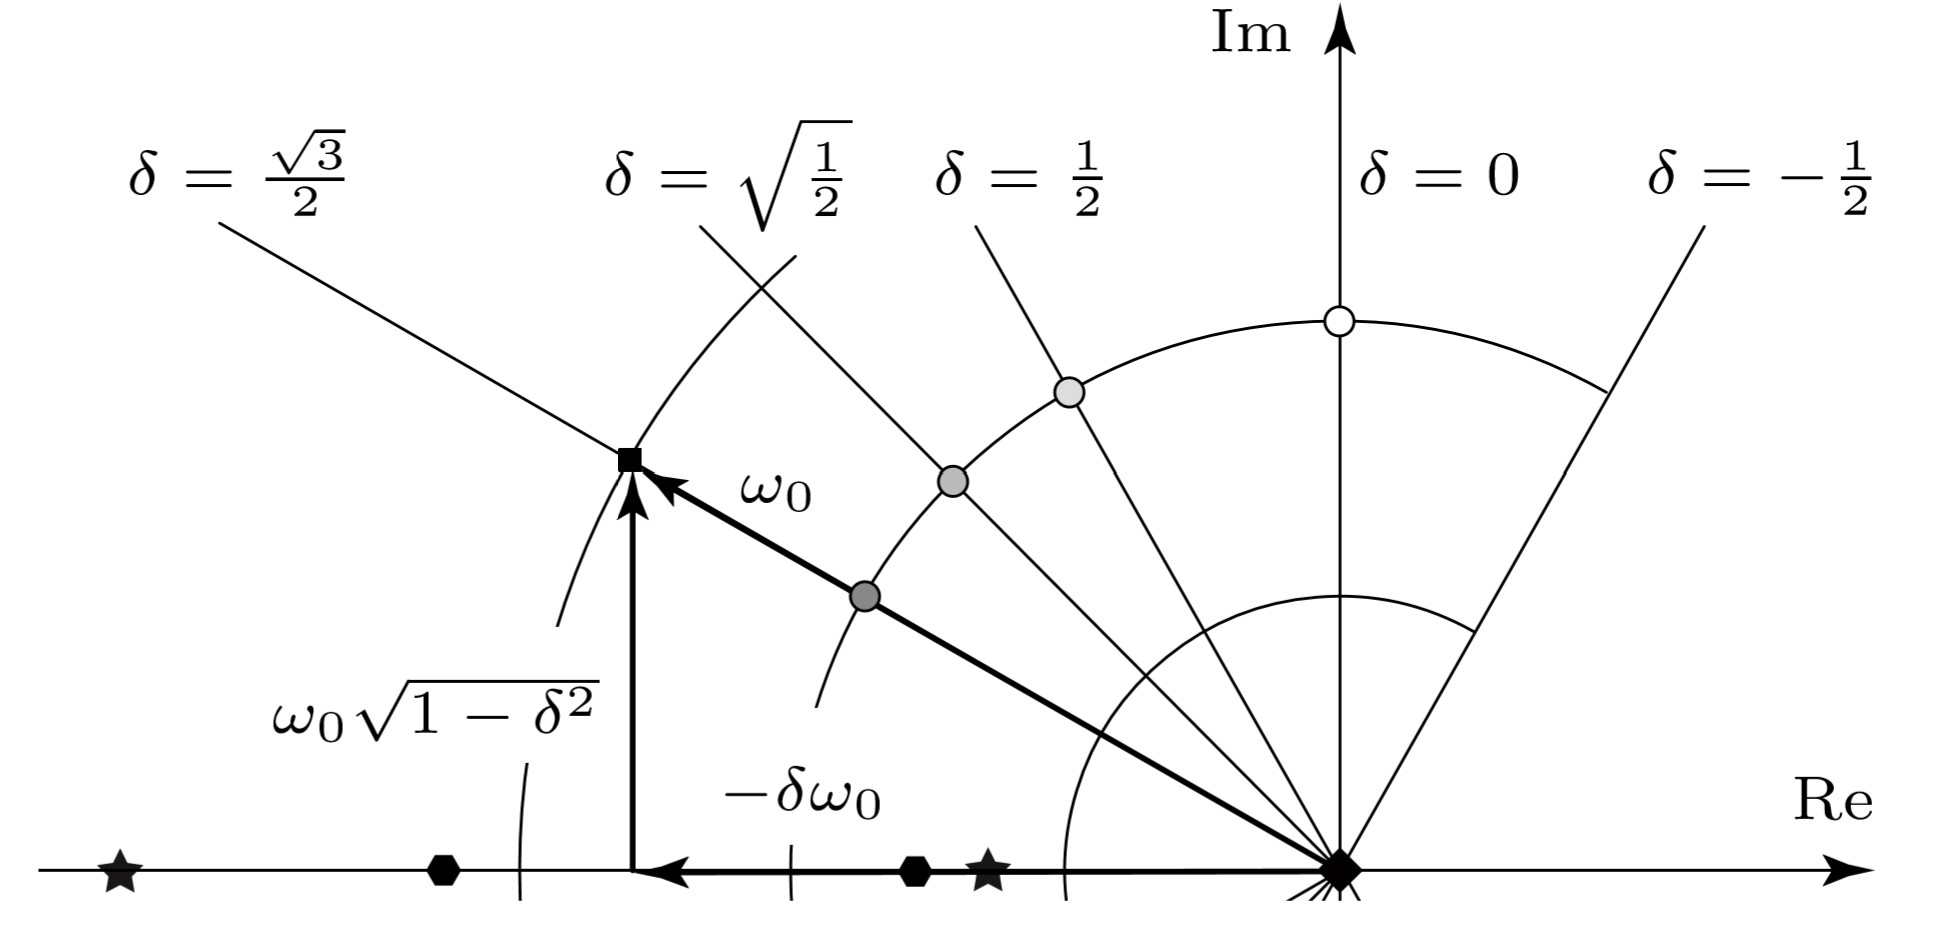
\includegraphics[width=\linewidth,height=45mm]{images/04/Anordnung_Polstellen.jpg}
        
        Dabei ist $\delta$ der \textbf{Dämpfungsparameter}. 
        Für $| \delta | < 1$ sind die Pole komplex.
        Für $| \delta | > 1$ sind die Pole rein reell.
        
        $\omega_0 = 2\pi/T_0$ ist die \textbf{natürliche Frequenz}, wobei $T_0$ die \textbf{natürliche Periode} ist.
        
        Abhängig von der Dämpfung gibt es drei grundsätzlich unterschiedliche Fälle des Systemsverhalten:
        
        $\boxed{ 0 < \delta < 1 }$  System enthält \textbf{Schwingungen}. 
        Die erste Schwingung überschiesst das Ziel $u(t) = h(t)$ um den Überschuss $\hat{\epsilon} = e^{-\delta\cdot\pi/\sqrt{1-\delta^2}},$ bei der Zeit $t^* =\frac{\pi}{\omega_0\cdot\sqrt{1-\delta^2}}$
        
        $\boxed{\delta > 1}$ Für \textbf{ungedämpfte Systeme} konvergiert das System, ähnlich wie bei einem System erster Ordnung zum Endwert. Die Systemantwort überschiesst in diesem Fall nicht. 
        
        $\boxed{ \delta = 1}$ Dieser Fall heisst \textbf{kritisch gedämpft} und entspricht der schnellst möglichen Konvergenz ohne Überschwinger.
        
        \begin{center}
            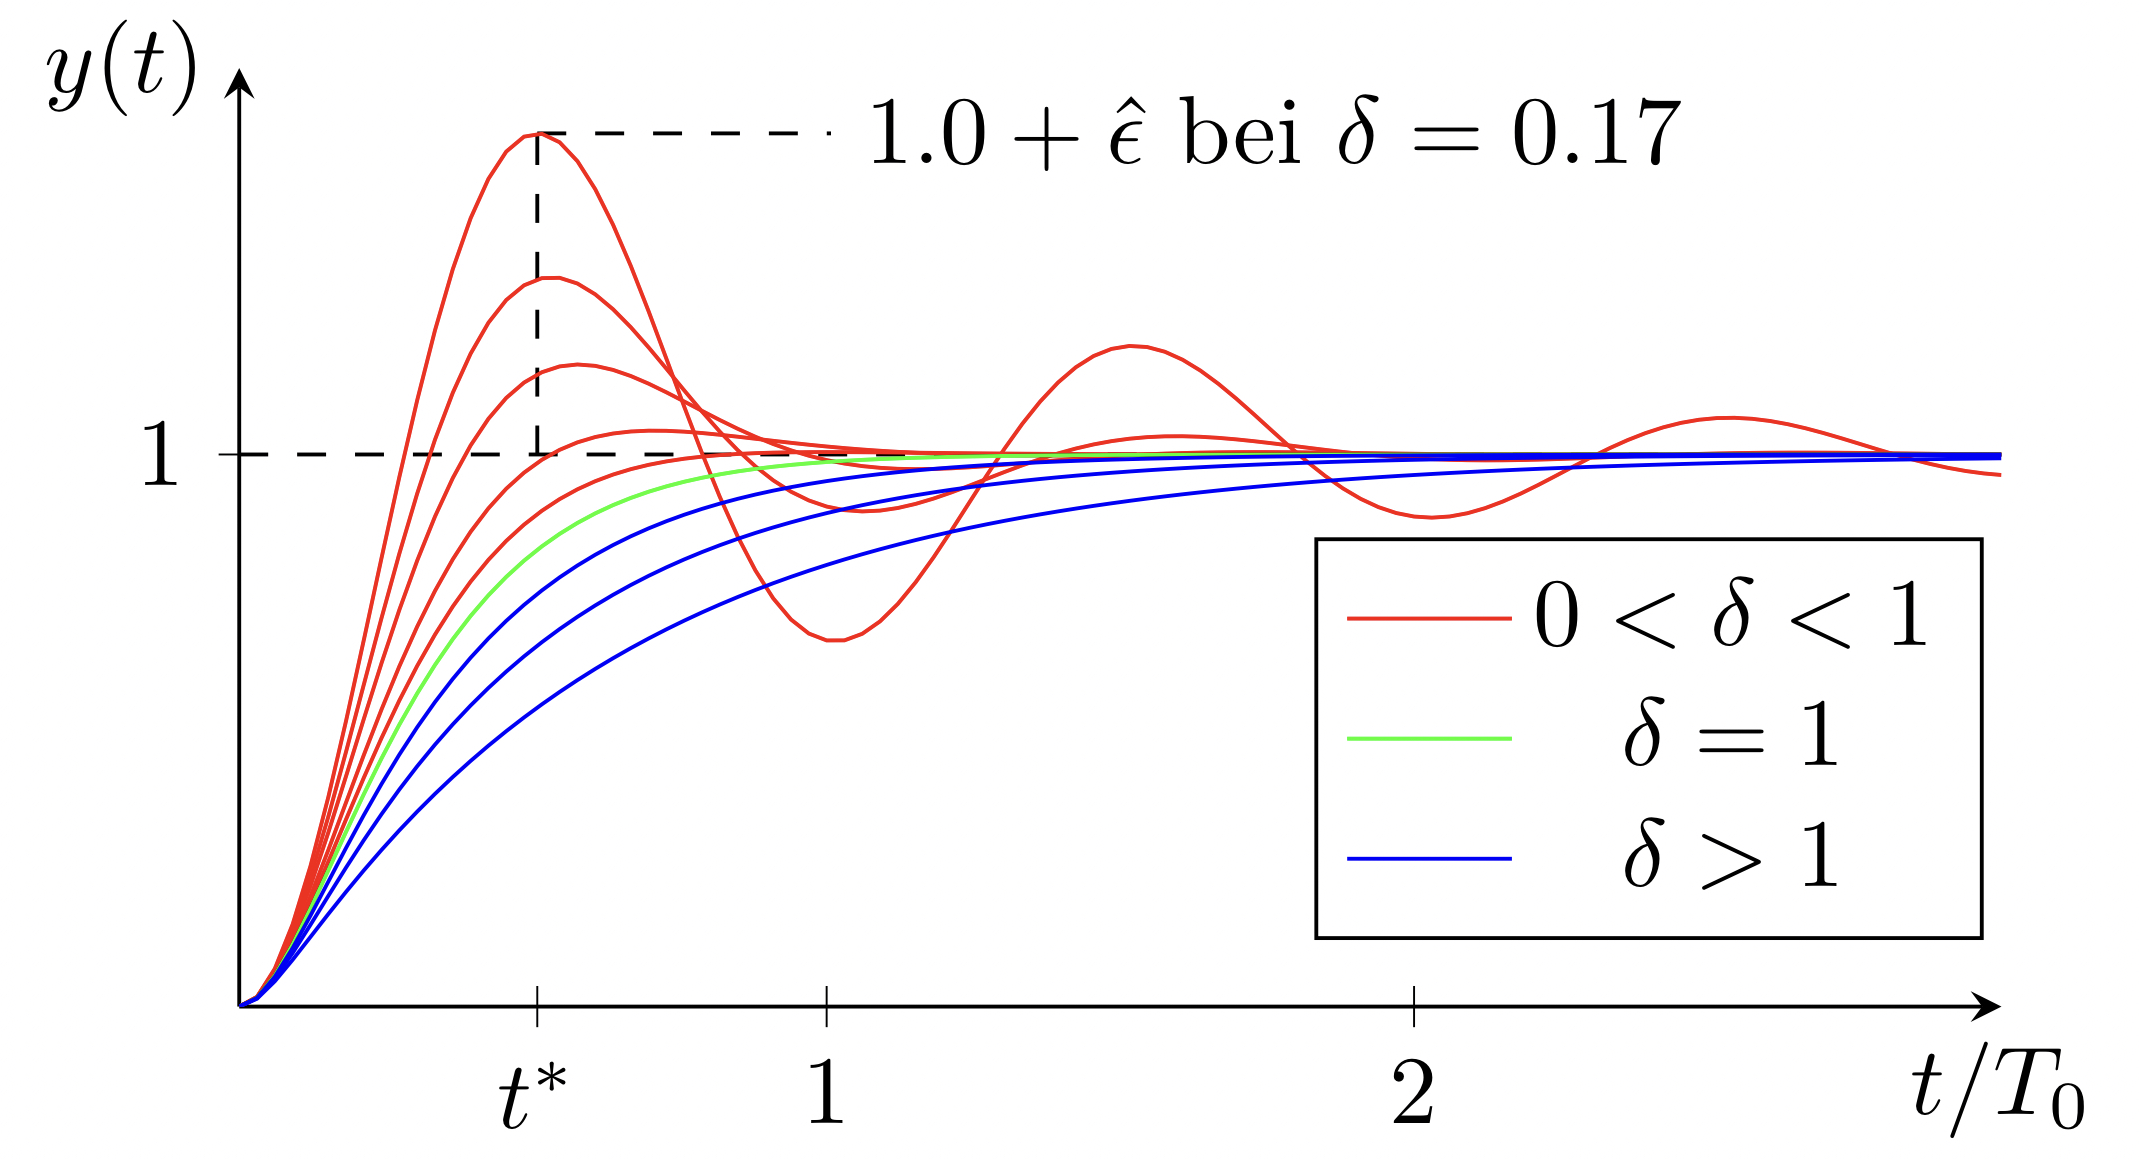
\includegraphics[width=0.55\linewidth]{04/dampening_sys_2.jpeg}
        \end{center}
        
        \subsubsection{Bsp Vereinfachung für $\delta>1$}
            \[\Sigma(s)= \frac{100}{s^2+101s+100}= \frac{100}{(s+100)(s+1)}\]
            Impulsantwort hat die Form: $\alpha\cdot e^{-100t}+\beta\cdot e^{-t}$. Da $e^{-100t}$ viel schneller abklingt als $e^{-t}$ kann man das System approximieren:
            \[\Sigma_{\textrm{approx}}(s)=\frac{1}{s+1}\]
            Man muss den Zähler anpassen, um die statische Verstärkung des approximierten Systems gleich zu halten: $\Sigma(0)= \Sigma_{\textrm{approx}}(0)$.
            \begin{center}
                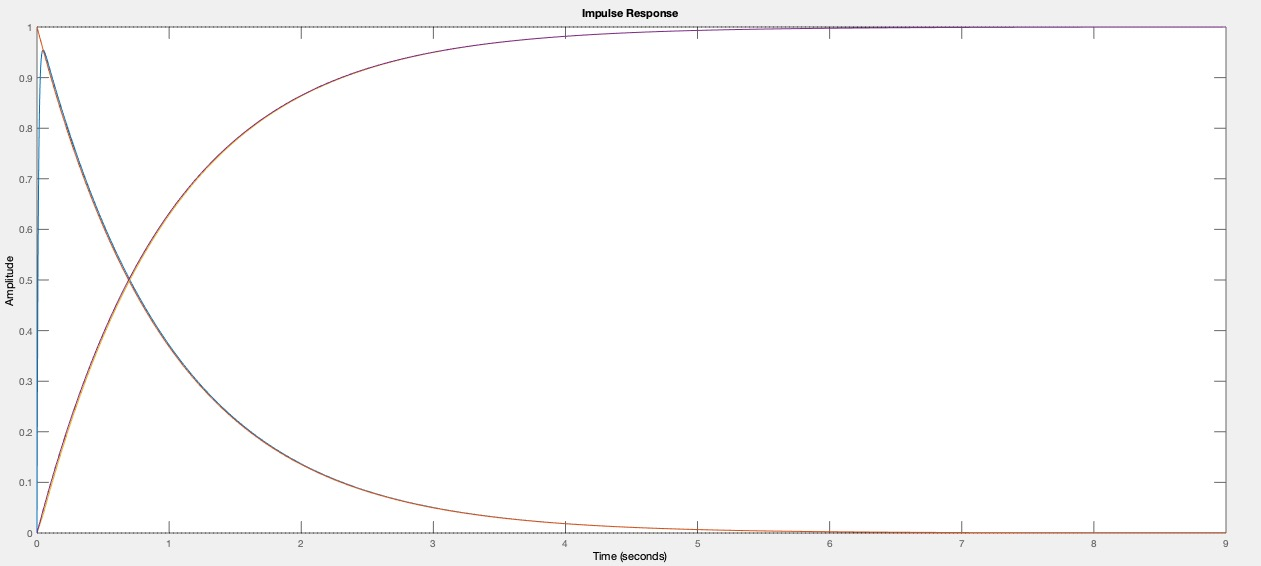
\includegraphics[width=\linewidth]{04/impulse_step_response_approx.jpg}
                \textit{Blau: Genaues System; Orange: Approximiertes System}
            \end{center}
        
        \subsection{Nullstelleneinfluss}
        \[\Sigma(s)=\frac{a\cdot s+1}{\dots}\]
        %Einfluss von Nullstellen auf das Systemverhalten.%
        Je näher die Nullstelle $\zeta = -1/a$ am Ursprung ist, desto stärker ist der Einfluss dieser Nullstelle. Dies widerspiegelt sich an einem stärkeren Überschuss in der Systemantwort. 
        Für $\zeta > 0 $ hat die Systemantwort einen \textbf{Undershoot}. Das heisst das System antwortet zuerst in die falsche Richtung. ein System mit einer Nullstelle der Form $\zeta > 0$ wird als \textbf{nicht-minimalphasig} bezeichnet.
        
        \textbf{Bemerkung:}
        Die initiale Sprungantwort in die `falsche' Richtung tritt bei einer ungeraden Anzahl positiver Nullstellen (Re($\zeta > 0))$ auf.
        \\Falls Steigung gleich 0 in $t=0$ ist, ist keine NST vorhanden
        
        \begin{center}
            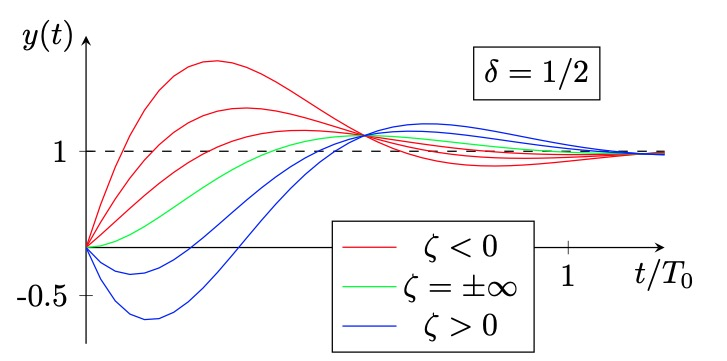
\includegraphics[width=0.8\linewidth]{04/NSTeinfluss.jpg}
        \end{center}
        
    \subsection{BIBO Stabilität}
        \textbf{BIBO} Stabilität bezieht sich auf das \textbf{I/O-Verhalten} von $\Sigma(S)$, wobei \textbf{Lyapunov Stabilität} sich auf das GGW der \textbf{Zustände} bezieht. 
        
        Ein System ist BIBO Stabil, falls für die Impulsantwort $\delta(t)$ folgendes gilt:
        \[\int_0^\infty|\delta(t)|dt < \infty\]
        \begin{itemize}
            \item Das System ist \textbf{BIBO stabil falls alle Pole $\pi_i$ negativen Realteil haben.}
            \item Das System ist nicht BIBO stabil in allen anderen Fällen.
        \end{itemize}
        
        Dabei ist wichtig, dass nicht beobachtbare Zustände und nicht steuerbare Zustände die BIBO Stabilität nicht beeinflussen, da sie sich in $\Sigma(s)$ wegkürzen. Obwohl BIBO und Lyapunov Stabilität sehr ähnlich wirken muss man sie auseinander halten, denn ein BIBO stabiles System kann Lyapunov instabil sein und ein Lyapunov stabiles System kann BIBO instabil sein.
 \vfill\null\columnbreak
        Für ein \textbf{komplett steuerbares und beobachtbares} ($\Leftrightarrow$ minimales) System gilt:
        \begin{center}
            \begin{tabular}{l c l}
                 asymptotisch stabil & $\rightarrow$ & BIBO stabil \\
                 asymptotisch stabil & $\leftarrow$ & BIBO stabil \\
                 Lyap. stabil oder instabil & $\rightarrow$ & BIBO instabil\\
                 Lyap. stabil oder instabil & $\leftarrow$ & BIBO instabil
            \end{tabular}
        \end{center}
        
        Für ein System, welches \textbf{\textit{nicht} komplett steuerbar und beobachtbar} ist gilt:
       \begin{center}
            \begin{tabular}{l c l}
                 asymptotisch stabil & $\rightarrow$ & BIBO stabil \\
                 ? & $\leftarrow$ & BIBO stabil \\
                 Lyap. stabil oder instabil & $\rightarrow$ & ?\\
                 Lyap. stabil oder instabil & $\leftarrow$ & BIBO instabil
            \end{tabular}
        \end{center}
        
        \subsubsection{Bsp}
            \[\dot{x}=
            \begin{bmatrix}
            -1 & 0 \\
            0 & 1
            \end{bmatrix}
            x+
            \begin{bmatrix}
            1 \\
            0
            \end{bmatrix}
            u, \quad y=\begin{bmatrix} 1 & 0 \end{bmatrix}x = x_1
            \]
            $\lambda_1=-1; \lambda_2=1$ Das System ist \textbf{Lyapunov instabil}. Nachvollziehbar für $x_2(0) \neq0$, dann divergiert der zustand $x_2\to\infty$. Da der instabile zustand weder steuerbar, noch beobachtbar ist, ist das System trotzdem BIBO stabil.
            \[\Sigma(s)=\frac{Y(s)}{U(s)}=\frac{1}{s+1}\]
            Der Pol hat einen negativen Realteil, ist also \textbf{BIBO Stabil} und gleichzeitig Lyapunov instabil.
        \subsection{Frequenzantworten}
        Zusätzlich zur \textbf{Sprung-} ($h(t)$) und der \textbf{Impuls-Eingangsgrösse} ($\delta(t)$) gibt es die \textbf{harmonische Eingangsgrösse}: \[u(t) = \alpha\cdot cos(\omega\cdot t + \Phi)\]
        
        wobei $\alpha$ die \textbf{Amplitude}, $\omega$ die \textbf{Frequenz} in $\frac{rad}{s}$, und $\Phi$ die \textbf{Phasenverschiebung} ist.
        
        der Ausgang eines Systems $\Sigma(s)$ mit harmonischen Eingang hat die Form:
        \[y(t) = y_{transient}(t) + y_\infty(t) \]
        Angenommen das System ist linear, zeitinvariant und asymptotisch stabil, gilt: 
        \[\displaystyle\lim_{t\to \infty} y_{transient}(t) \rightarrow 0 \Rightarrow y(t) \rightarrow y_{\infty}\]
        
        Die asymptotische Systemantwort ist eine verstärkter und phasenverschobener Cosinus bei derselben Frequenz wie der Eingang: 
        \[y_{\infty}(t) = m(\omega)\cdot \alpha \cdot cos(\omega \cdot t + \Phi + \varphi(\omega))\]
        
        die Verstärkung $m(\omega)$ und die Phasenverschiebung $\varphi(\omega)$ sind systemabhängig. Es gilt:
        \[y_{\infty}(t) = |\Sigma(j\omega)| \cdot \alpha \cdot cos(\omega\cdot t+ \Phi + \angle \Sigma(j\omega)\]
        
        D.h die Verstärkung entspricht der Systemverstärkung bei der Eingangsfrequenz und die Phasenverschiebung entspricht der Systemphase bei der Eingangsfrequenz. 
        
        \textbf{Wichtig!} Lineare Systeme generieren keine neue Frequenzen. Es kommen immer dieselben Frequenzen aus dem System, wie in das System gehen. D.h die Phasenverschiebung und Verstärkung ist nur frequenzabhängig und somit eine Eigenschaft des Systems.
        
        \[\left|\Sigma_1(S)\cdot\Sigma_2(S)\right| = \left|\Sigma_1(S)\right|\cdot\left|\Sigma_2(S)\right|\]
        \[\angle(\Sigma_1(S)\cdot\Sigma_2(S)) = \angle\Sigma_1(S)+\angle\Sigma_2(S)\]
        
\vfill\null\columnbreak
\section{Visualisierung}  
    \[u(t)=cos(\omega t) \Rightarrow y(t)=|P(jw)|\cdot cos(\omega t+\angle P(j\omega))\]
  \subsection{Bode Diagramme}
        Die Magnitude und Phase wird gegenüber einer logarithmischen Frequenzskala eingezeichnet.
        Dabei ist die Magnitude üblicherweise in Dezibel, und Die Phase in Grad dargestellt.
        
        \textbf{Umrechnung zwischen dezimal und dezibel:}
        
        \[|\Sigma(s)|_{dB} = 20 \cdot \textrm{log}_{10}|\Sigma(s)|= 20\cdot\frac{\textrm{ln}(|\Sigma(s)|)}{\textrm{ln}(10)}\]
        \[|\Sigma(s)| = 10^{\frac{|\Sigma(s)|_{dB}}{20}}\]
        
        \begin{center}
        {\renewcommand{\arraystretch}{1.4}
            \begin{tabular}{c|c}
        
            Dezimalskala    &   Dezibelskala [dB]\\
            \hline
            100 &   40  \\
            10  &   20  \\
            5   &   13.97..\\
            3.16.. & 10\\
            2   &   6.02..\\
            1   &   0   \\
            $\frac{1}{\sqrt{2}}$  &   -3.0103\\
            0.316.. & -10\\
            0.1 &   -20 \\
            0.01    &   -40\\
            0       &   $-\infty$
            \end{tabular}}
        \end{center}
        \[|\Sigma(j\omega)|_{dB} = |\Sigma_1(j\omega)|_{dB}+|\Sigma_2(j\omega)|_{dB}\]
        \[\angle\Sigma= \angle\Sigma_{1}+ \angle\Sigma_{2}\]
        \[\angle\Sigma(j\omega)=
        \begin{cases}
            \arctan(\frac{x}{y}) & x > 0\\
            \arctan(\frac{x}{y})+\pi & x<0
      \end{cases}
      \]
                 
        \subsubsection{Systeme 1. Ordnung}
            Viele reale Regelkreise können als Systeme erster Ordnung approximiert werden. Ein solches System reagiert auf tiefe Frequenzen, die kleiner als die Eckfrequenz (Cutoff Frequency) $\omega_c = \frac{1}{\tau}$ sind. Bei Anregungsfrequenzen höher als $\omega_c$ verhindert die Trägheit des Systems eine starke Änderung des Ausgangs. Ausserdem reagiert das System für $\omega > \omega_c$ zunehmend verzögert, wie an der Phase des Bode Diagramms ersichtlich ist. Eine wichtiges Merkmal: die Magnitude bei $\omega_c = \frac{1}{\tau}$ ist immer bei $\frac{1}{\sqrt{2}}\approx -3 dB.$
            \begin{center}
                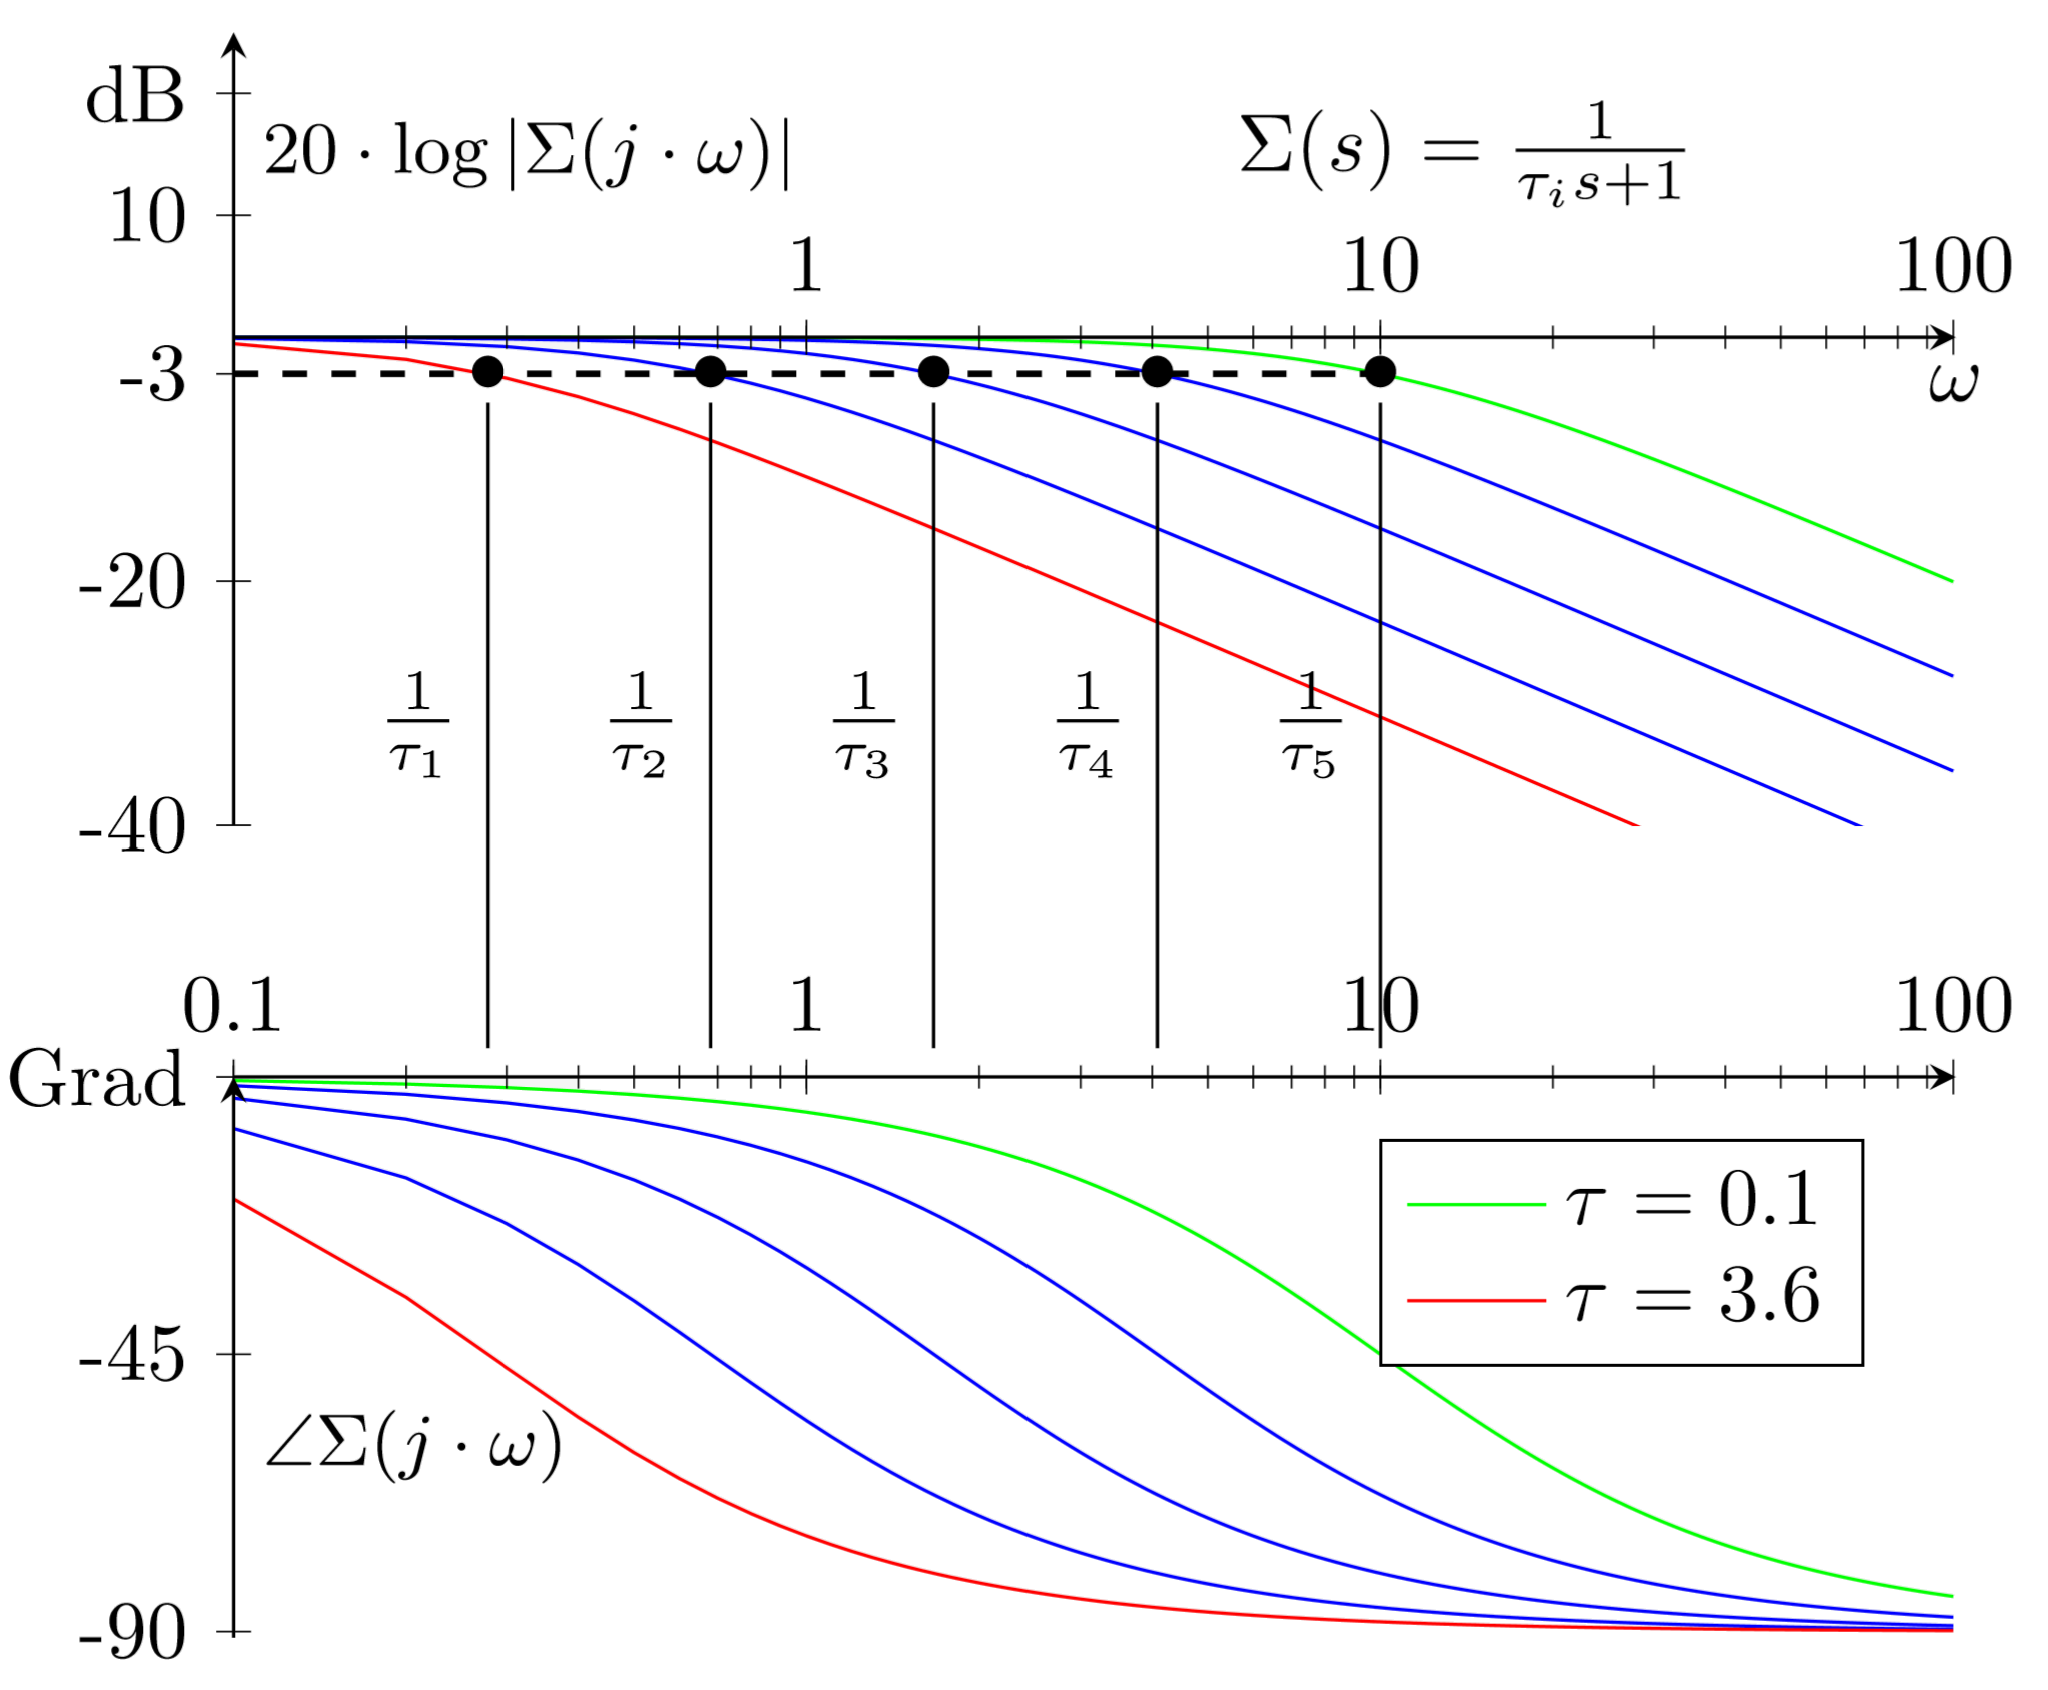
\includegraphics[width = 0.8\linewidth]{images/05/Bode_1Ordnung.png}
            \end{center}
        \subsubsection{Systeme 2. Ordnung}
            Viele mechanischen Systeme zeigen resonantes Verhalten (grössere Verstärkung bei mittleren Frequenzen als bei tiefen - eine sogenannte Resonanzüberhöhung). Solche Systeme werden oft als Systeme zweiter Ordnung approximiert.
            \begin{center}
                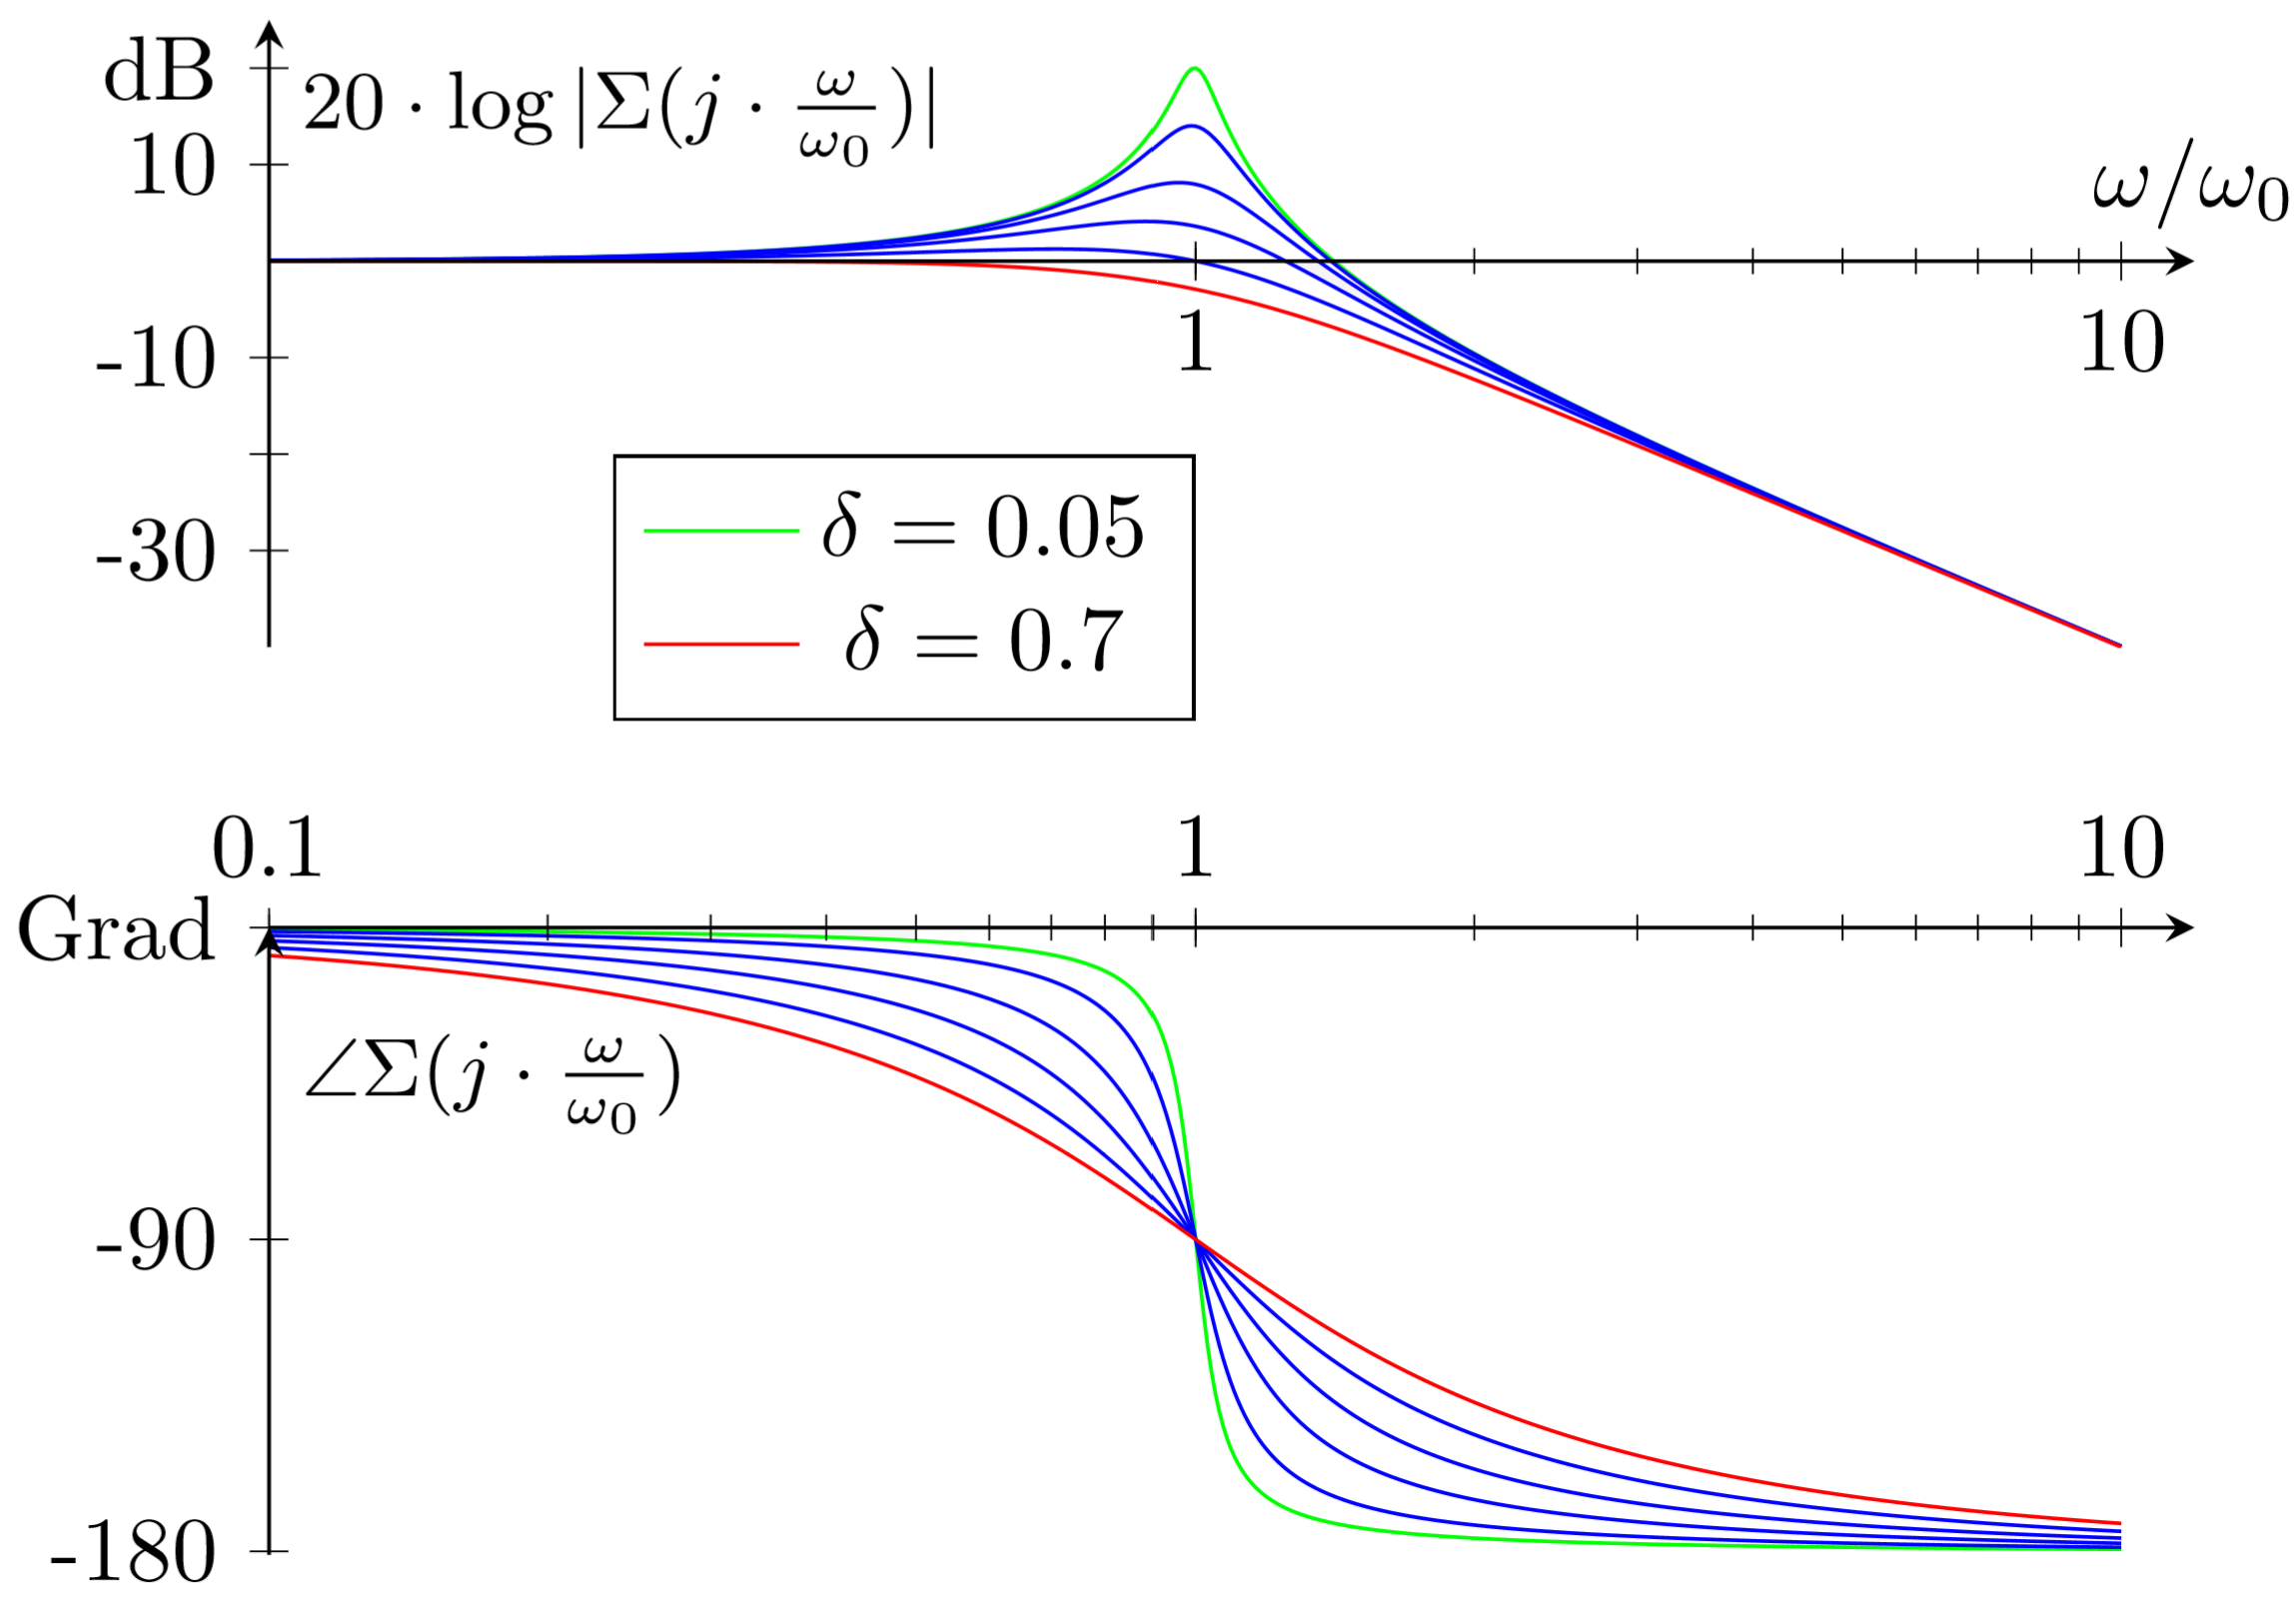
\includegraphics[width = 0.8\linewidth]{images/05/Bode_2Ordnung.png}
            \end{center}
            \textbf{Vorsicht!} Die resonante Frequenz (maximale Verstärkung) ist nicht bei der natürlichen Frequenz $\frac{\omega}{\omega_0} = 1$, sondern bei:
            \[\omega_{max} = \omega_0\cdot\sqrt{1-2\cdot\delta^2}, \hspace{4mm} 0<\delta<\frac{1}{\sqrt{2}}
            \]
            jedoch gilt für kleine Dämpfungsparameter $\omega_{max}\approx\omega_0.$ 
            Ausserdem zeigen Systeme 2. Ordnung für $\delta > \frac{1}{\sqrt{2}}$ kein resonantes Verhalten.
        \subsubsection{Einfluss von Polen \& Nullstellen auf das Bode Diagramm}
            {\renewcommand{\arraystretch}{1.4}
                \begin{tabular}{l|c|c}
                Standardelemente    &   Verstärkung $[\frac{dB}{dec}]$   &   Phase\\
                \hline
                Stabiler Pol    &   $-20$ bei $\omega_c$  &   $-90^{\circ}$ bei $\omega_c$\\
                Instabiler Pol    &   $-20$ bei $\omega_c$  &   $+90^{\circ}$ bei $\omega_c$\\
                Minimalphasige NST    &   $+20$ bei $\omega_c$  &   $+90^{\circ}$ bei $\omega_c$\\
                \small{Nichtminimalphasige NST}    &   $+20$ bei $\omega_c$  &   $-90^{\circ}$ bei $\omega_c$\\
                Delay um $\tau(\forall\omega)$ &    0   &   $-\frac{180}{\pi}\cdot\omega\cdot\tau^{\circ}$
            \end{tabular}}
    
        \subsubsection{Bsp}
            Zeichne Bode-Plot von $\Sigma(s)=\frac{100s}{(10s+1)(s+10)}$.
            \textbf{Vorgehen:}
            \begin{enumerate}
                \item In Standardelemente Zerlegen:
                \[\Sigma(s)=(100s)(\frac{1}{10s+1})(\frac{1}{s+10})\]
                \item NST/Pole der Standardelemente bestimmen:
                \[\zeta_1=0;\quad \pi_2=-\frac{1}{10};\quad\pi_3=-10\]
                \item Betrag der NST/Pole bestimmen.
                \[w_{\zeta}=|\zeta_1|=0;\quad w_{c_2}=|\pi_2|=\frac{1}{10};\quad w_{c_3}|\pi_3|=10\]
                \item $\Sigma(0)$ der einzelnen Elemente bestimmen.
                \[\Sigma_1(10^{-3})=0.1=-20dB;\quad \Sigma_2(0)=1=0dB;\]
                \vspace{-5mm}\[\Sigma_3(0)=\frac{1}{10}=-20dB\]
                \item Bode-Plot zeichnen 
            \end{enumerate}
            \begin{center}
                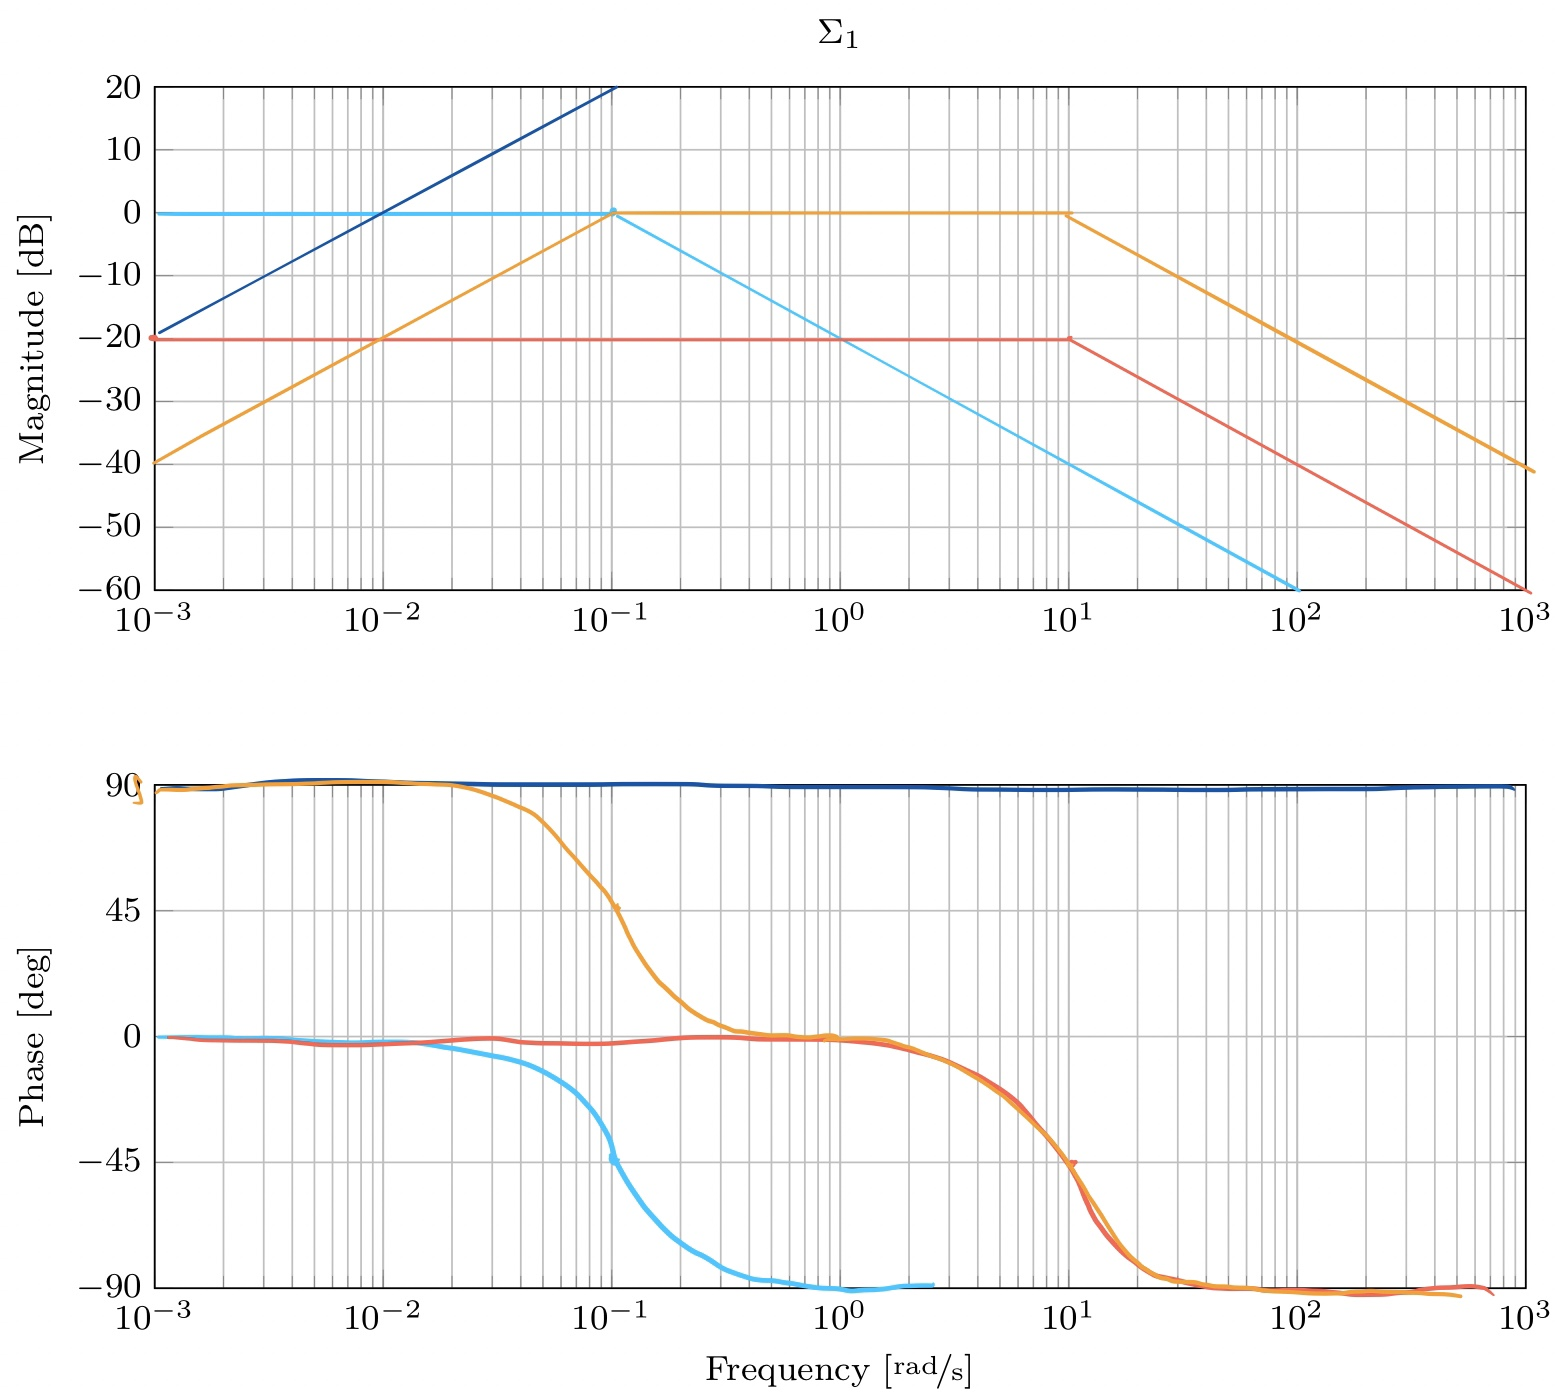
\includegraphics[width=0.6\linewidth]{05/bsp_bode.jpeg}
                \\\textit{Lösung in Orange}
            \end{center}
        \subsubsection{Bsp}
            Identifiziere Übertragungsfunktion in der From $\Sigma(s)=k\frac{s-\zeta}{s-\pi}$.
            \begin{center}
                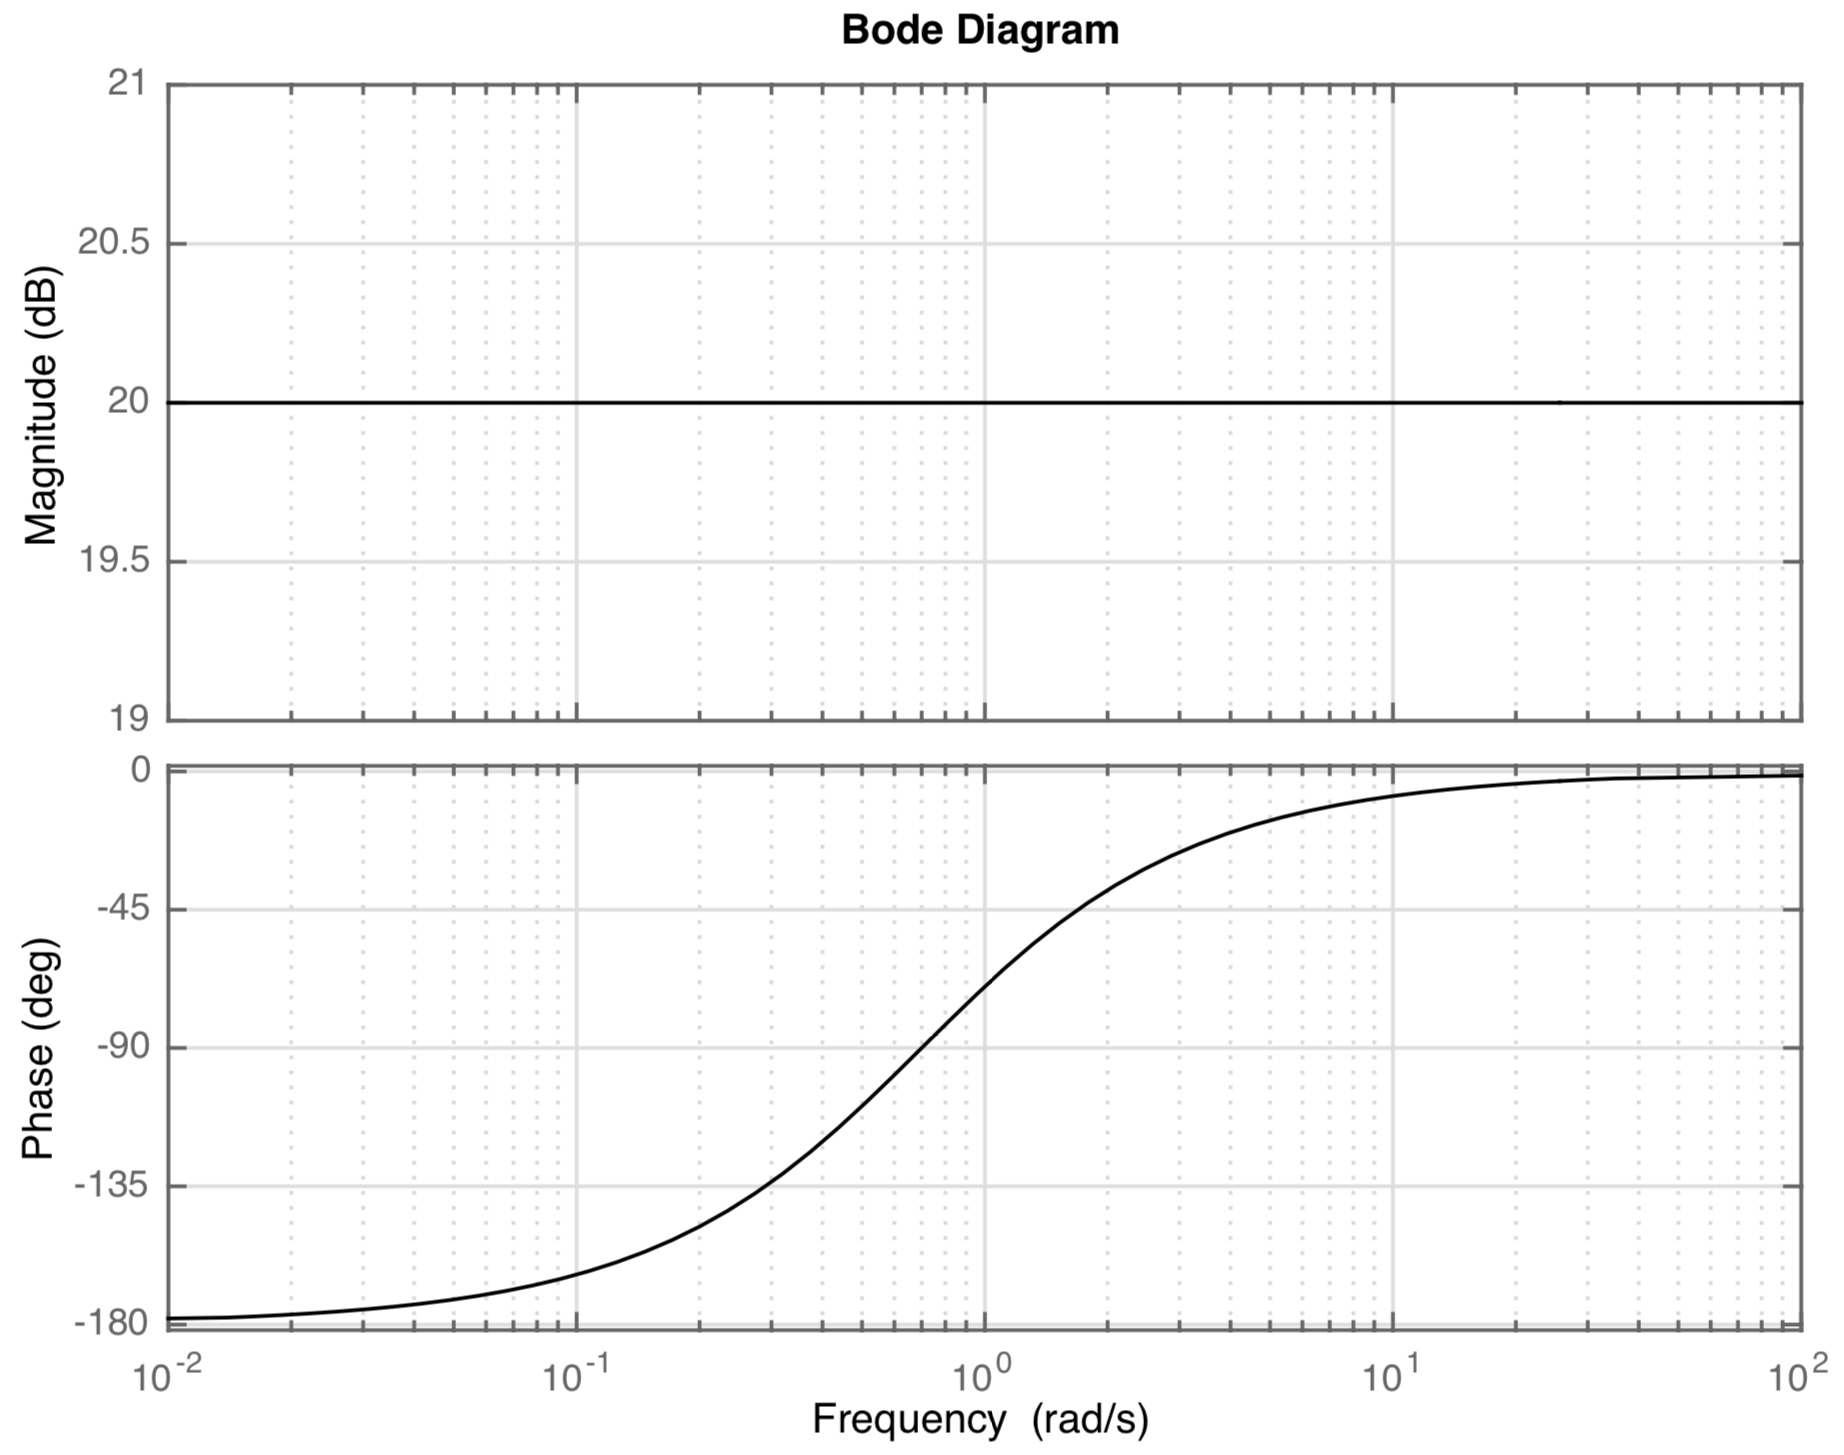
\includegraphics[width=0.47\linewidth]{05/neg_stat_gain.jpeg}
                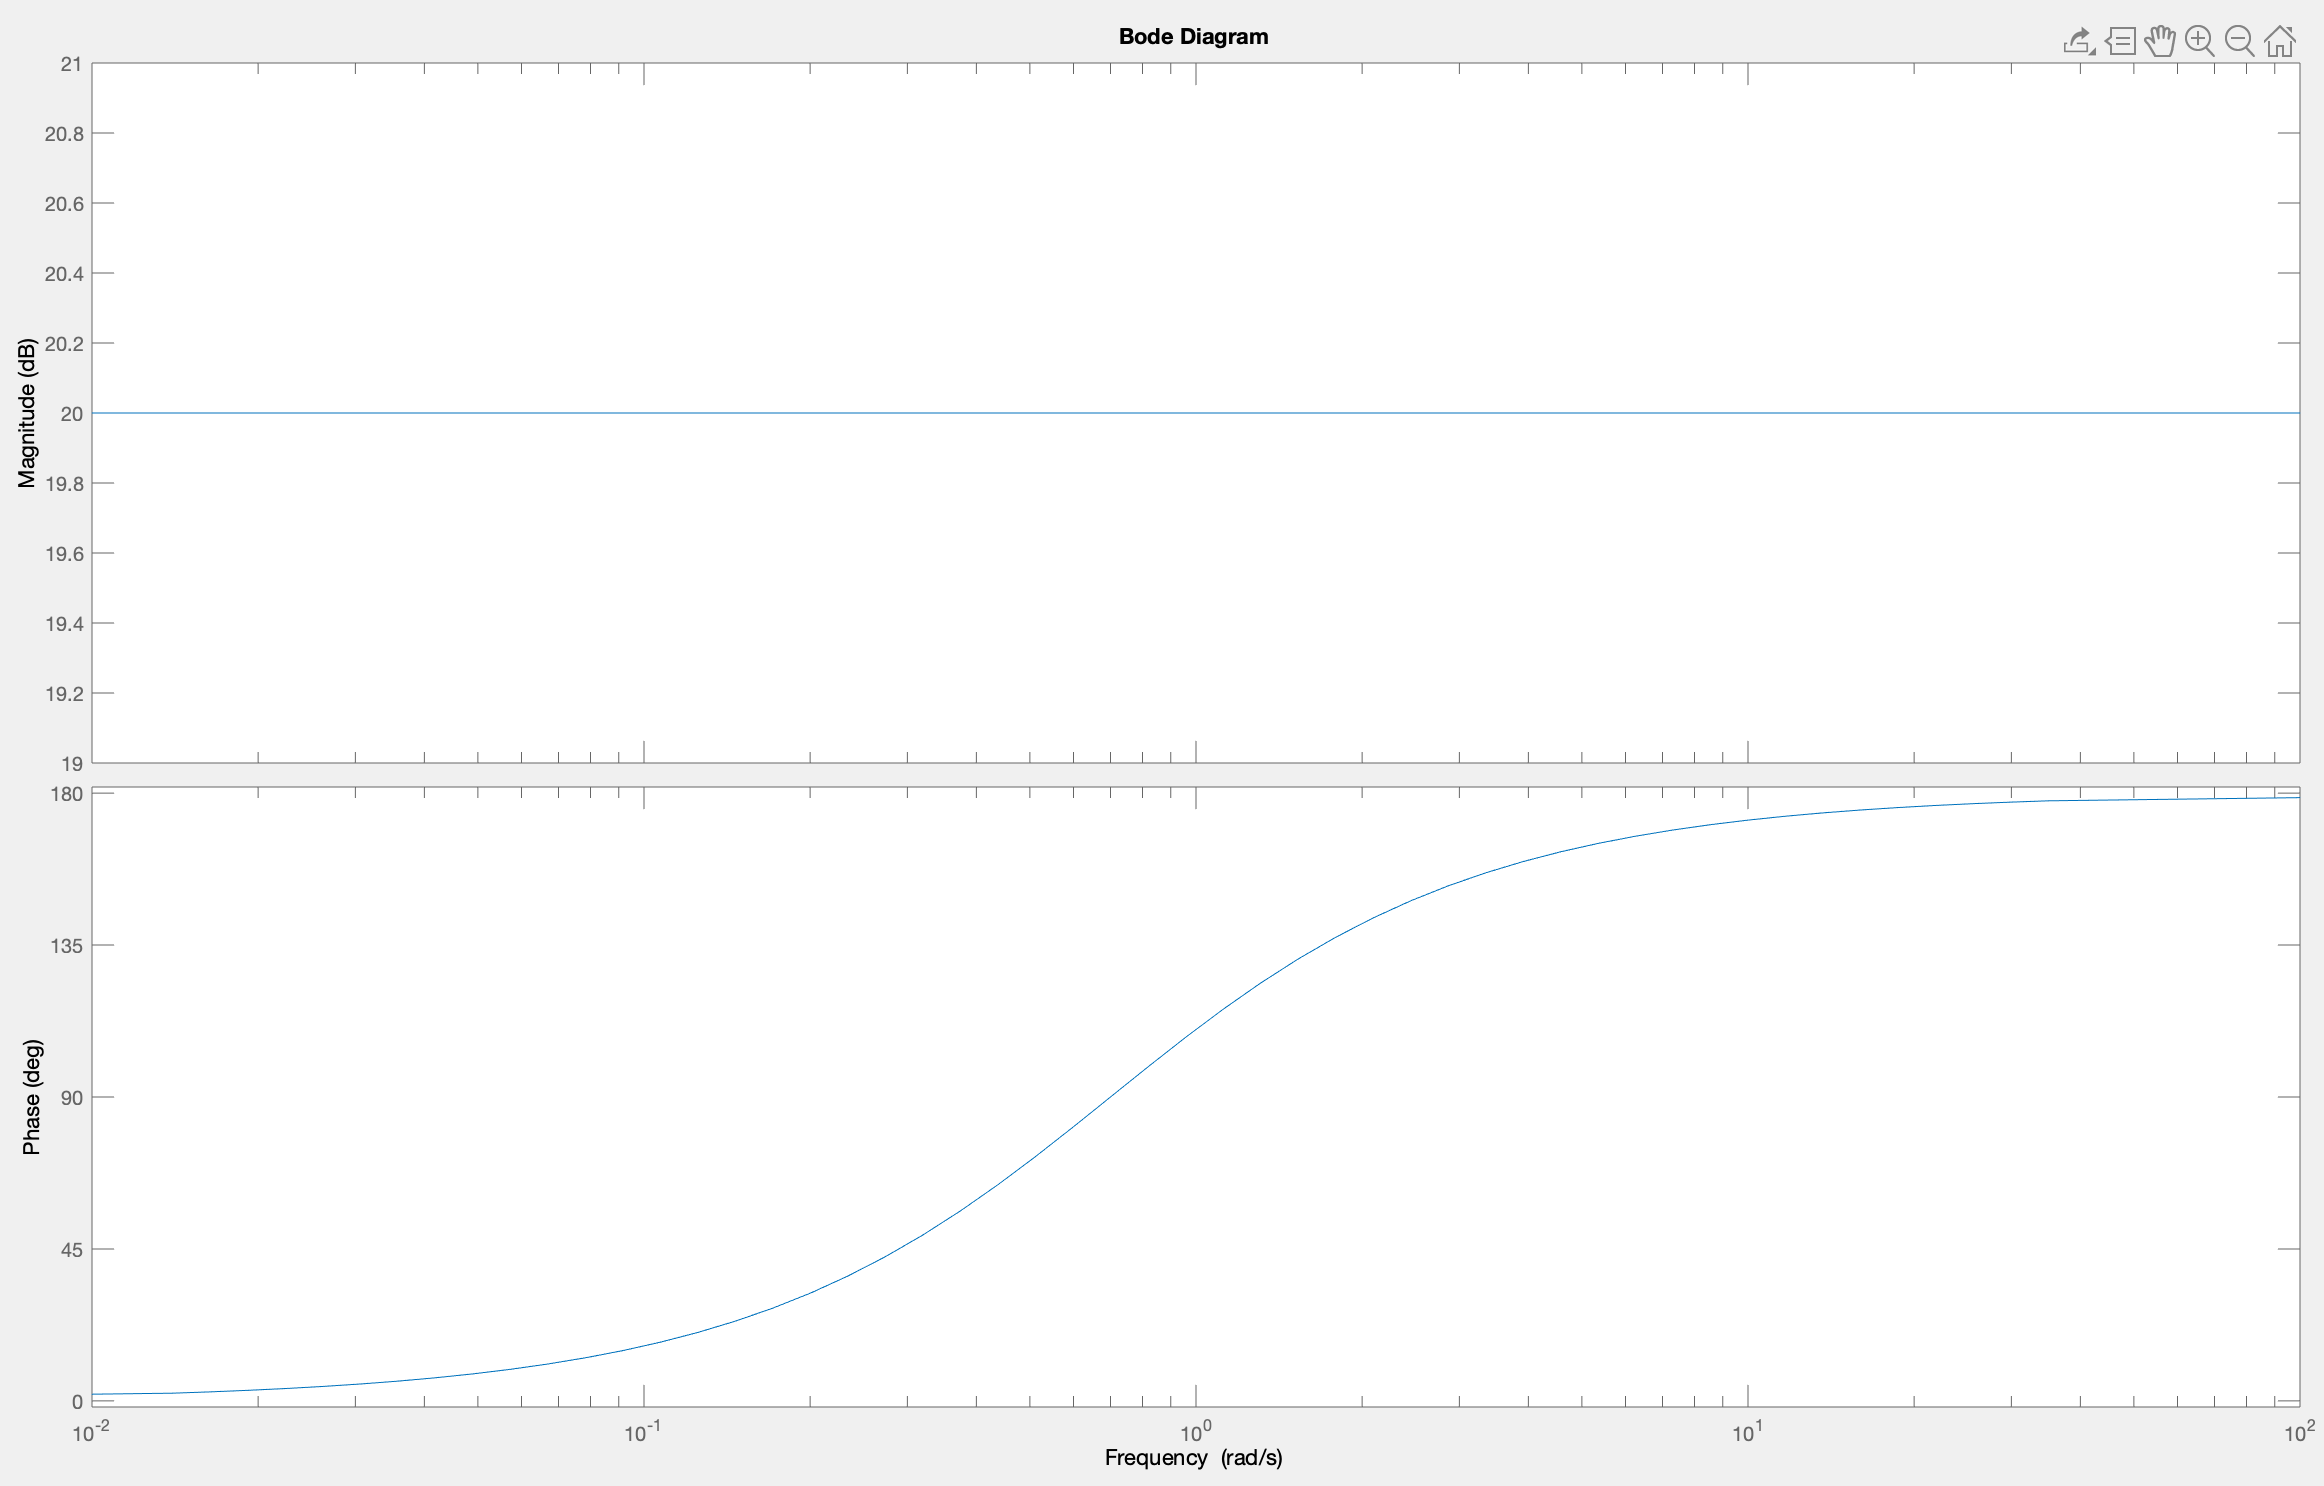
\includegraphics[width=0.5\linewidth]{images/05/neg_stat_gain_2.png}
                \small{\textit{Links: $\Sigma(s)$ mit negativer statischer Verstärkung}\\
                \textit{Rechts: $-1\cdot\Sigma(s)=:\Sigma(s)_{pos}$ mit positiver statischer Verstärkung}}
            \end{center}
            \begin{enumerate}
                \item $|\Sigma(s)|=20dB \quad\forall\omega$ $\rightarrow$ Pol und Nullstelle müssen an der selben Stelle sein. Da das System eine neg. stat. Verstärkung hat rechnen wir das gesamte System mal $-1$. Dadurch gewinnt das System $180^{\circ}$ Phase. So können wir das System aus Standardelementen darstellen.
                \item System gewinnt an $180^{\circ}$ Phase $\rightarrow$ eine stabile NST und ein instabiler Pol.
                \item Auslesen aus Bode Plot ergibt für $|\pi|=|\zeta|=0.7$ und $|\Sigma(s)_{pos}|=k\frac{\sqrt{\omega^2+0.7^2}}{\sqrt{\omega^2+0.7^2}} \Rightarrow k=20dB=10$
                \item $\Sigma(s)_{pos}=-10\frac{s+0.7}{s-0.7} \Leftrightarrow \Sigma(s)=10\frac{s+0.7}{s-0.7}$
            \end{enumerate}
                \begin{center}
                    \textbf{Falls Anzahl mini-phasige NST + instabile Pole \textit{ungerade}, hat das System neg. stat. Verstärkung}
                \end{center}
                
                
    \subsection{Nyquist Diagramme}
        Darstellung des Frequenzganges (Magnitude und Phase über die Anregungsfrequenz $\omega$) in der komplexen Ebene.
        \subsubsection{Systeme 1. Ordnung}
        Ein allgemeines System 1. Ordnung bei der Frequenz $s= j\omega$ hat folgende Magnituden und Phasen, wobei $\tau = \frac{1}{\omega_c} $:
        \[|\Sigma(j\omega)| = \frac{1}{\sqrt{\tau^2\omega^2+1}}
        \qquad
        \angle\Sigma(j\omega) = -arctan(\tau\cdot\omega)
         \]
        \begin{center}
        \vspace{-2mm}
            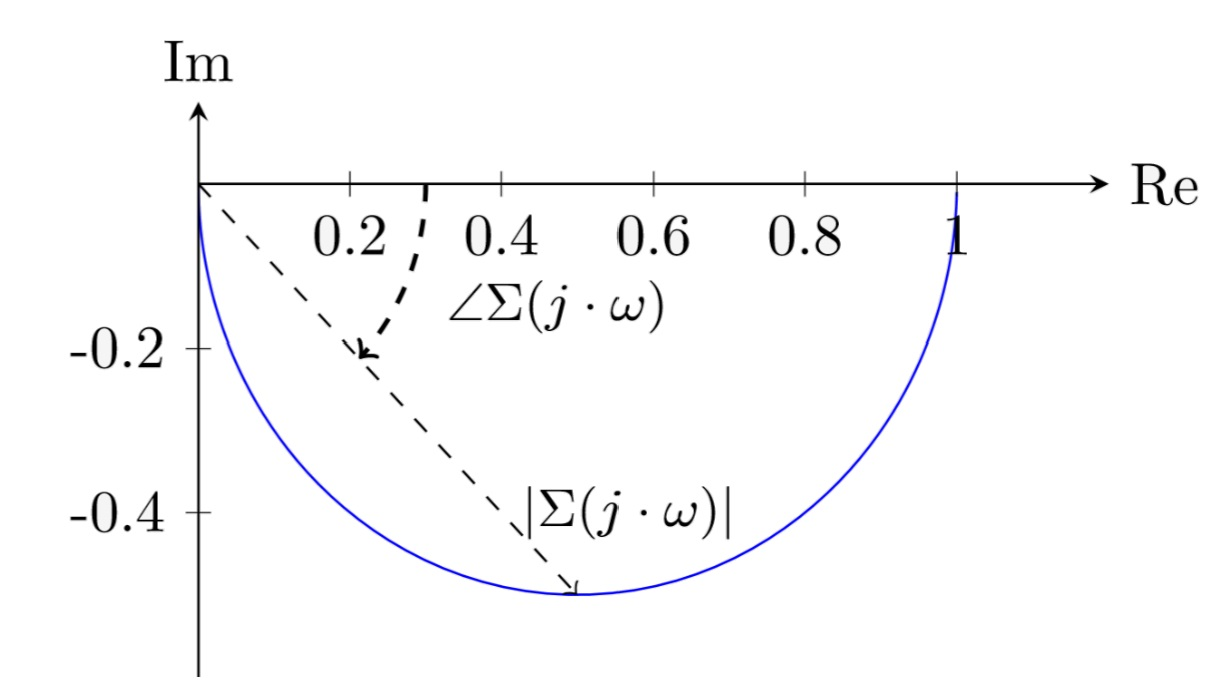
\includegraphics[width=0.6\linewidth ]{images/05/Nyq_1Ordnung.jpg}
        \end{center}
        \textbf{Bemerkung:} Für alles Systeme 1. Ordnung $\displaystyle\Sigma(s)=\frac{k}{T\cdot s+1}$ mit $\omega\in(-\infty,\infty)$ ist die Nyquist-Kurve ein Kreis mit Mittelpunkt $(k/2,0)$.
    
        \subsubsection{Systeme 2. Ordnung}
            Ein allgemeines System 2. Ordnung hat bei der Frequenz $s=j\cdot\omega$ folgende Magnituden und Phasen:
            \[ |\Sigma(j\omega)| = \frac{\omega_0^2}{\sqrt{(\omega_0^2-\omega^2)^2+4\cdot \delta^2 \cdot \omega_0^2\cdot \omega^2}}\]
            \[
            \angle\Sigma(j\omega) = \begin{cases} -arctan(\dfrac{2\cdot\delta\cdot\omega_0\cdot\omega}{\omega_0^2-\omega^2}) & \forall 0 \leq \omega \leq\omega_0 \\
            \\  
            -arctan(\dfrac{2\cdot\delta\cdot\omega_0\cdot\omega}{\omega_0^2-\omega^2}) -\pi & \forall \omega_0 < \omega
            
            \end{cases}
            \]
            \begin{center}
                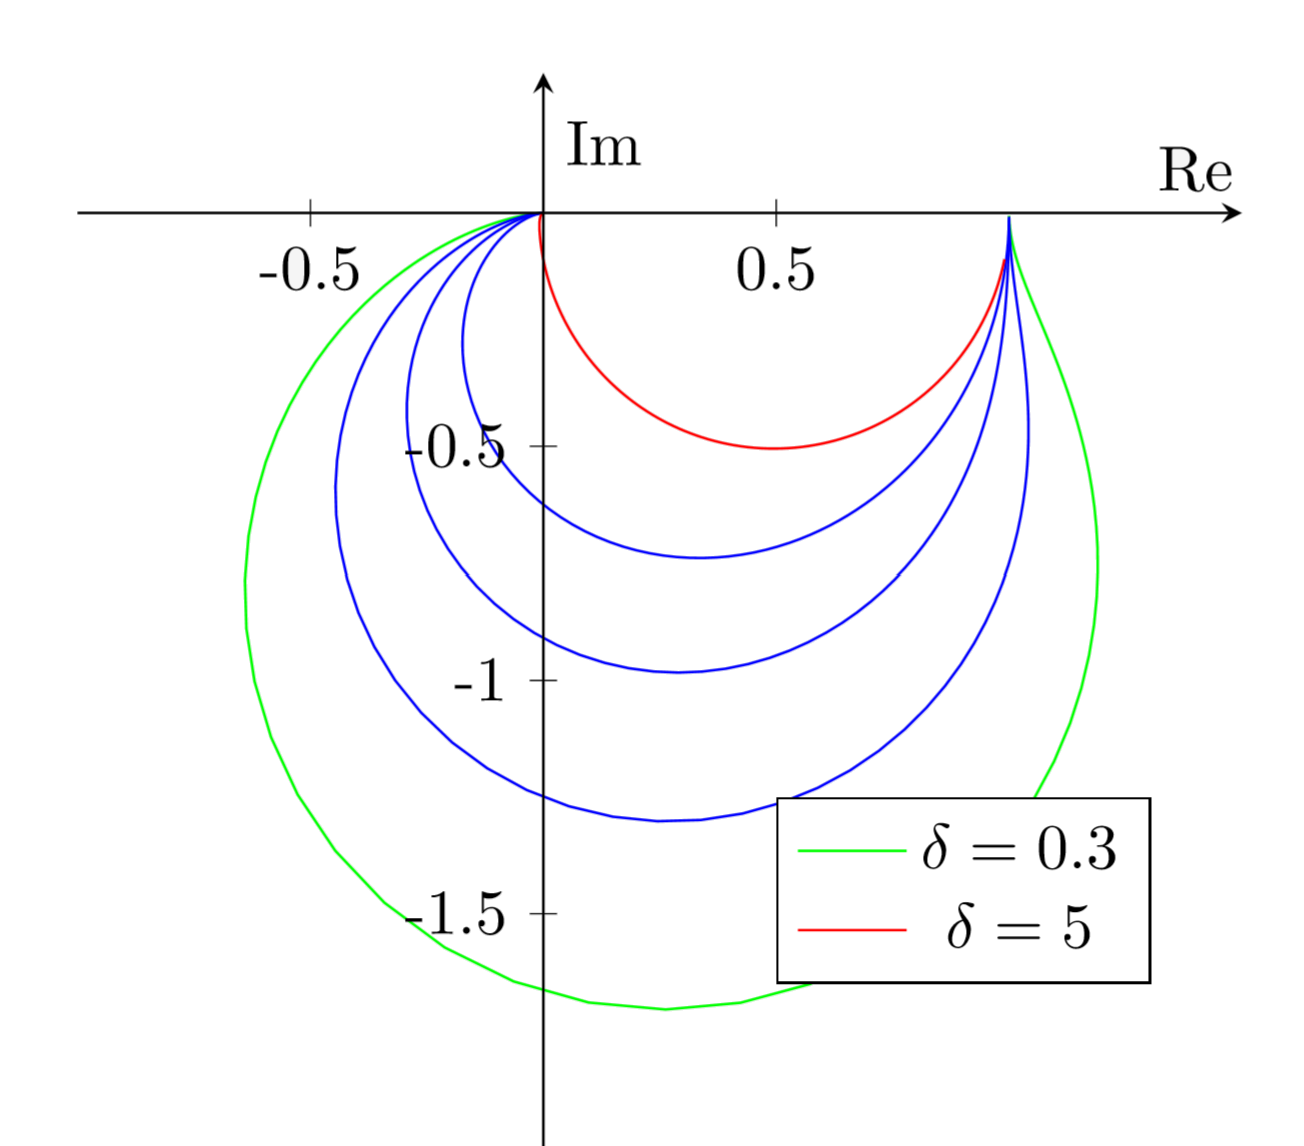
\includegraphics[width = 0.5\linewidth]{images/05/Nyq_2Ordnung.jpg}
            \end{center}

        \subsubsection{Bsp}
            Gegeben sei eine Kreisverstärkung $\frac{1}{s^2+s+1}$
            man will $\angle L(j\omega)$ für $\omega \rightarrow \infty$ herausfinden.
            \textbf{Achtung!} nicht einfach einsetzten und ausmultiplizieren! stattdessen zwei Nullststellen ausfindig machen und dann einsetzen. 
            
            \textbf{Für sehr hohe Frequenzen gilt:}
            \begin{center}
                \renewcommand{\arraystretch}{1.3}{\begin{tabular}{l|c}
                  offener Integrator $\frac{1}{s^k}$   & $\displaystyle\lim_{\omega\to\infty}\angle L(j\omega)= -k\cdot \frac{\pi}{2}$ \\
                   \#instabiler Pol   & \#$+\frac{\pi}{2}$ \\
                   \#stabiler Pol & \#$-\frac{\pi}{2}$\\
                   \#minimalphasige Nullstelle &   \#$+\frac{\pi}{2}$\\
                   \#Nicht-minimalphasige Nullstelle & \#$-\frac{\pi}{2}$
                \end{tabular}}
            \end{center}
        
         \subsubsection{Bsp}
            \begin{center}
                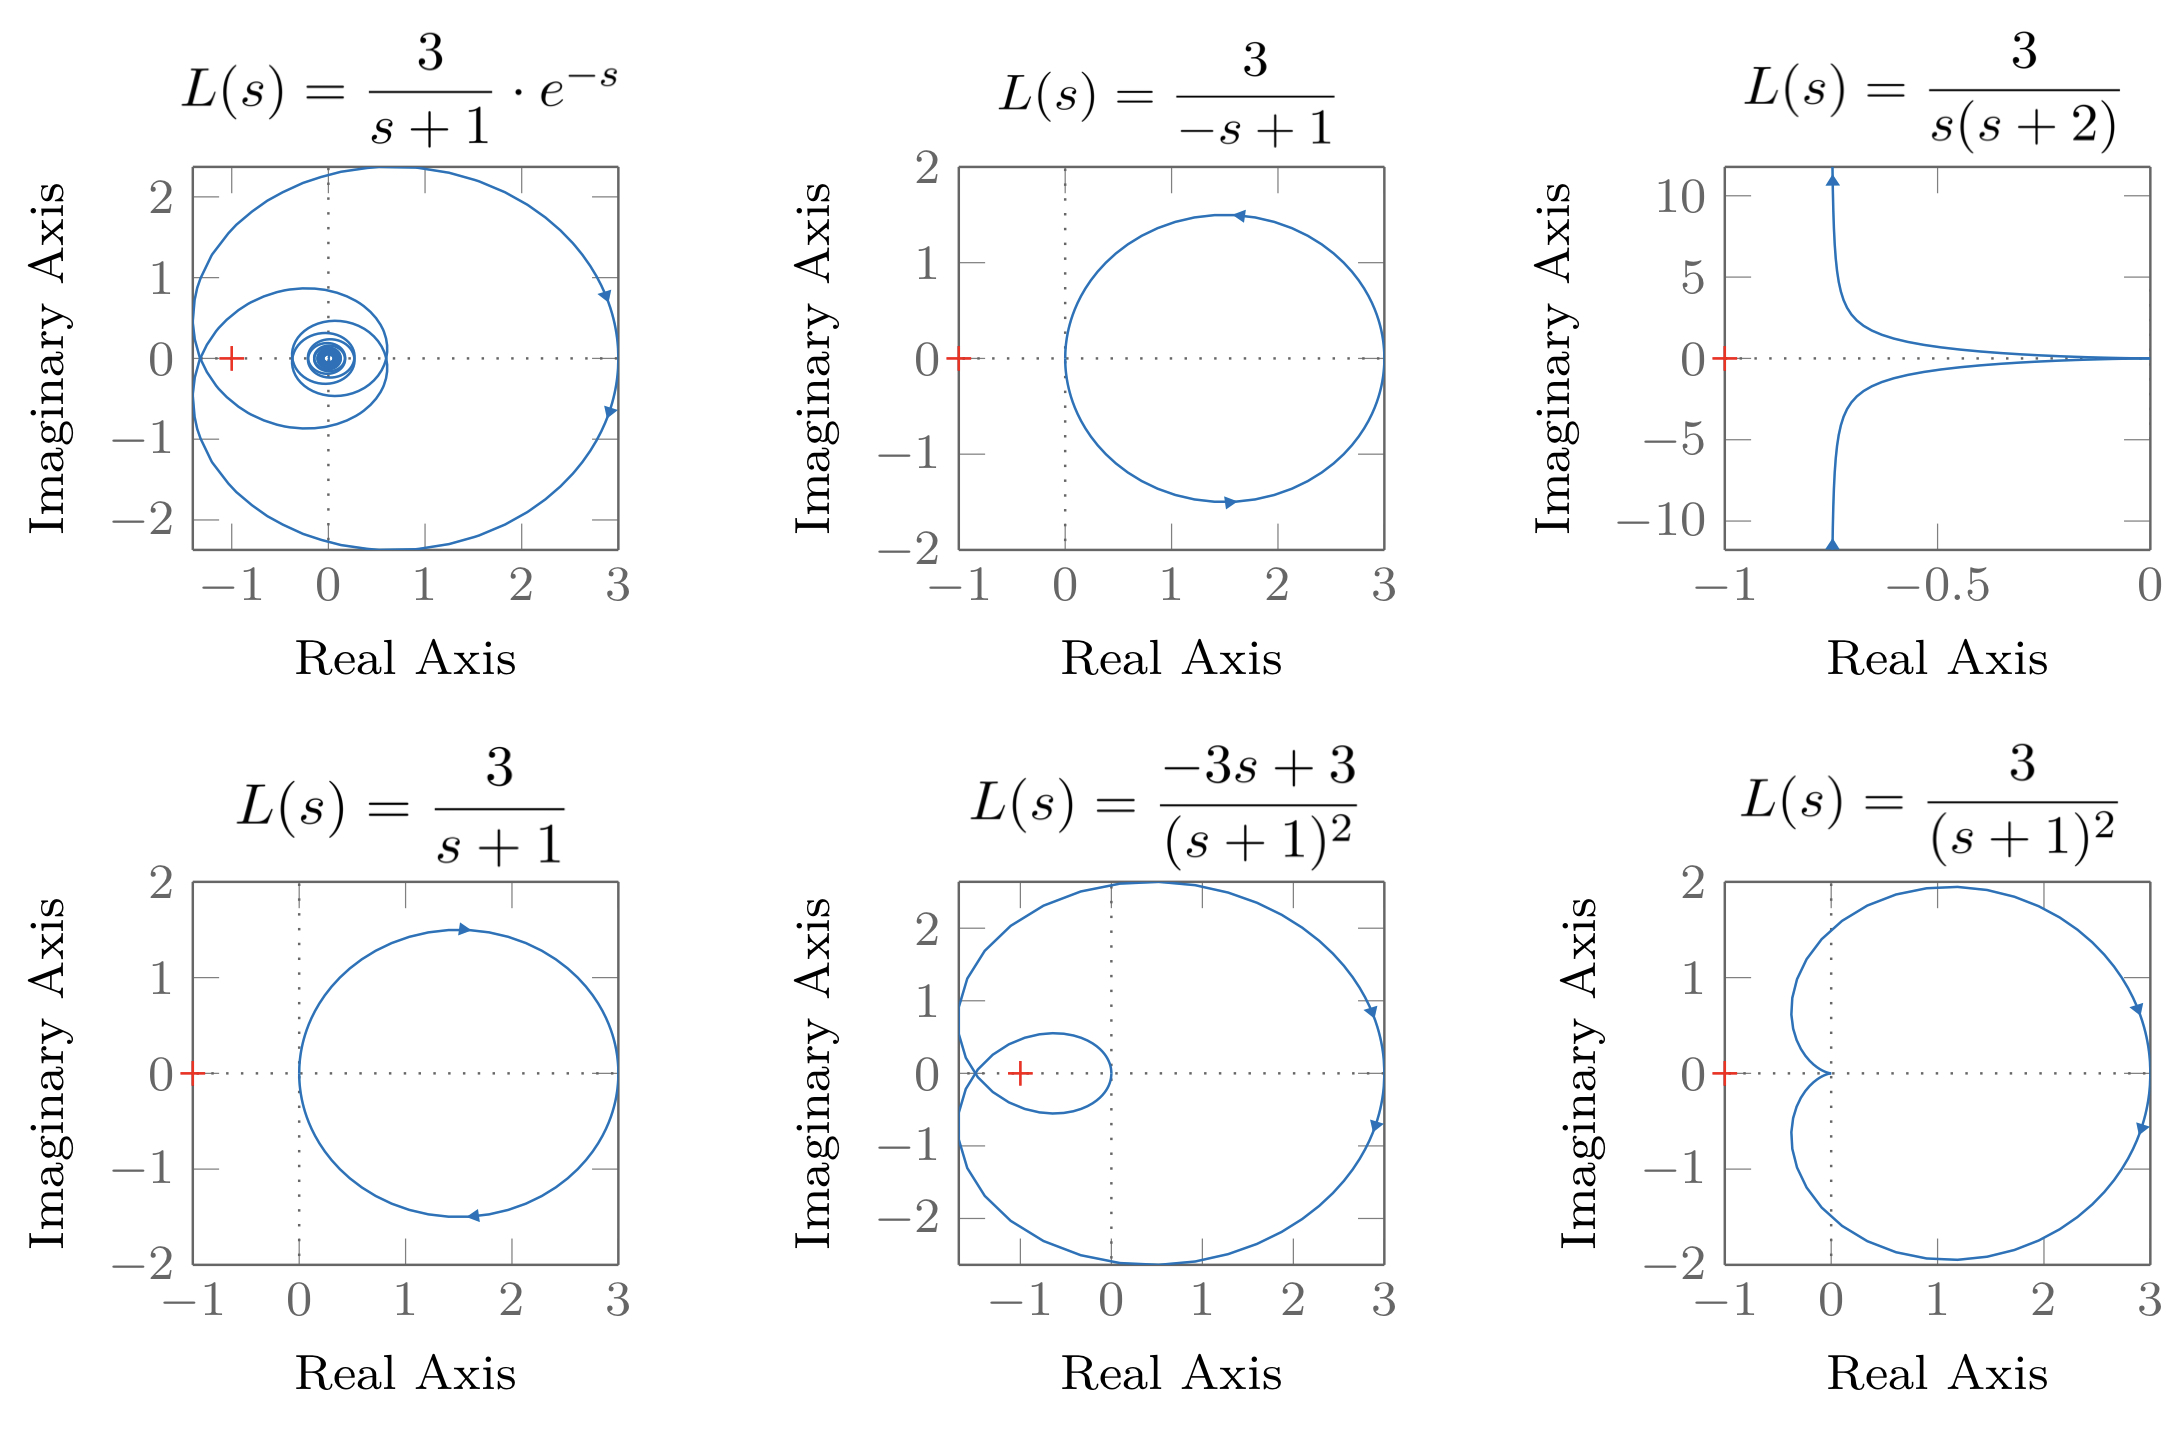
\includegraphics[width=\linewidth]{images/05/bsp_nyquist.jpeg}
                \textit{Einige Übertragungsfunktionen und ihre Nyquist-Diagramme}
            \end{center}
            
    \subsection{Asymptotische Eigenschaften von Frequenzantworten}
        Gegeben sei die folgender Struktur einer allgemeinen Übertragungsfunktion:
        \[\Sigma(s) = \frac{b_m\cdot s^{\mathbf{m}}+\hdots + b_1 \cdot s + b_0}{s^{\mathbf{k}}\cdot (s^{\mathbf{n}-k}+a_{n-1-k}\cdot s^{n-1-k}+\hdots+ a_1 \cdot s + a_0)}\]
        Aus der Übertragungsfunktion kann man direkt die \textbf{Phase} bei $\omega = 0$ aus dem \textbf{Systemtyp} $k$ bestimmen. 
        Zusätzlich kann man das Asymptotische Verhalten der Magnitude $|\Sigma(j\omega)|$ für $\omega \rightarrow \infty$ direkt aus dem \textbf{relativen Grad} $ r=n-m$ bestimmen.
        
        \subsubsection{Systemtyp $k$}
        Der \textbf{Systemtyp $k$} entspricht der Vielfachheit offener Integratoren $\frac{1}{s^k}$ des Systems. Die Phase bei $\omega = 0$ lässt sich folgendermassen bestimmen.
        
        \[\angle\Sigma(0) =  \begin{cases}
        -k\cdot \frac{\pi}{2}, & sgn(\frac{b_0}{a_0}) > 0 \\
        -\pi-k\cdot \frac{\pi}{2}, & sgn(\frac{b_0}{a_0}) < 0 \textrm{ (neg. stat. Gain)}
        \end{cases}\]
        
        \subsubsection{Relativer Grad $r = n - m$}
        Die Steigung des Magnitudenverlauf im Bode-Diagramm konvergiert asymptotisch zu: 
        \[\frac{\partial|\Sigma(j\omega)|_{dB}}{\partial log(\omega)} = -r\cdot 20\frac{dB}{decade}\]
        
        \subsection{Modellunsicherheit}
            Ein Modell eines physikalischen Systems kann das wahre System nicht perfekt reproduzieren. Durch die Berücksichtigung der maximal zu erwartenden Modellierungsunsicherheit beim Entwurf eines Regelsystems kann robustes Verhalten garantiert werden.
            \subsubsection{Nichtparametrische Unsicherheit}
            \begin{center}
                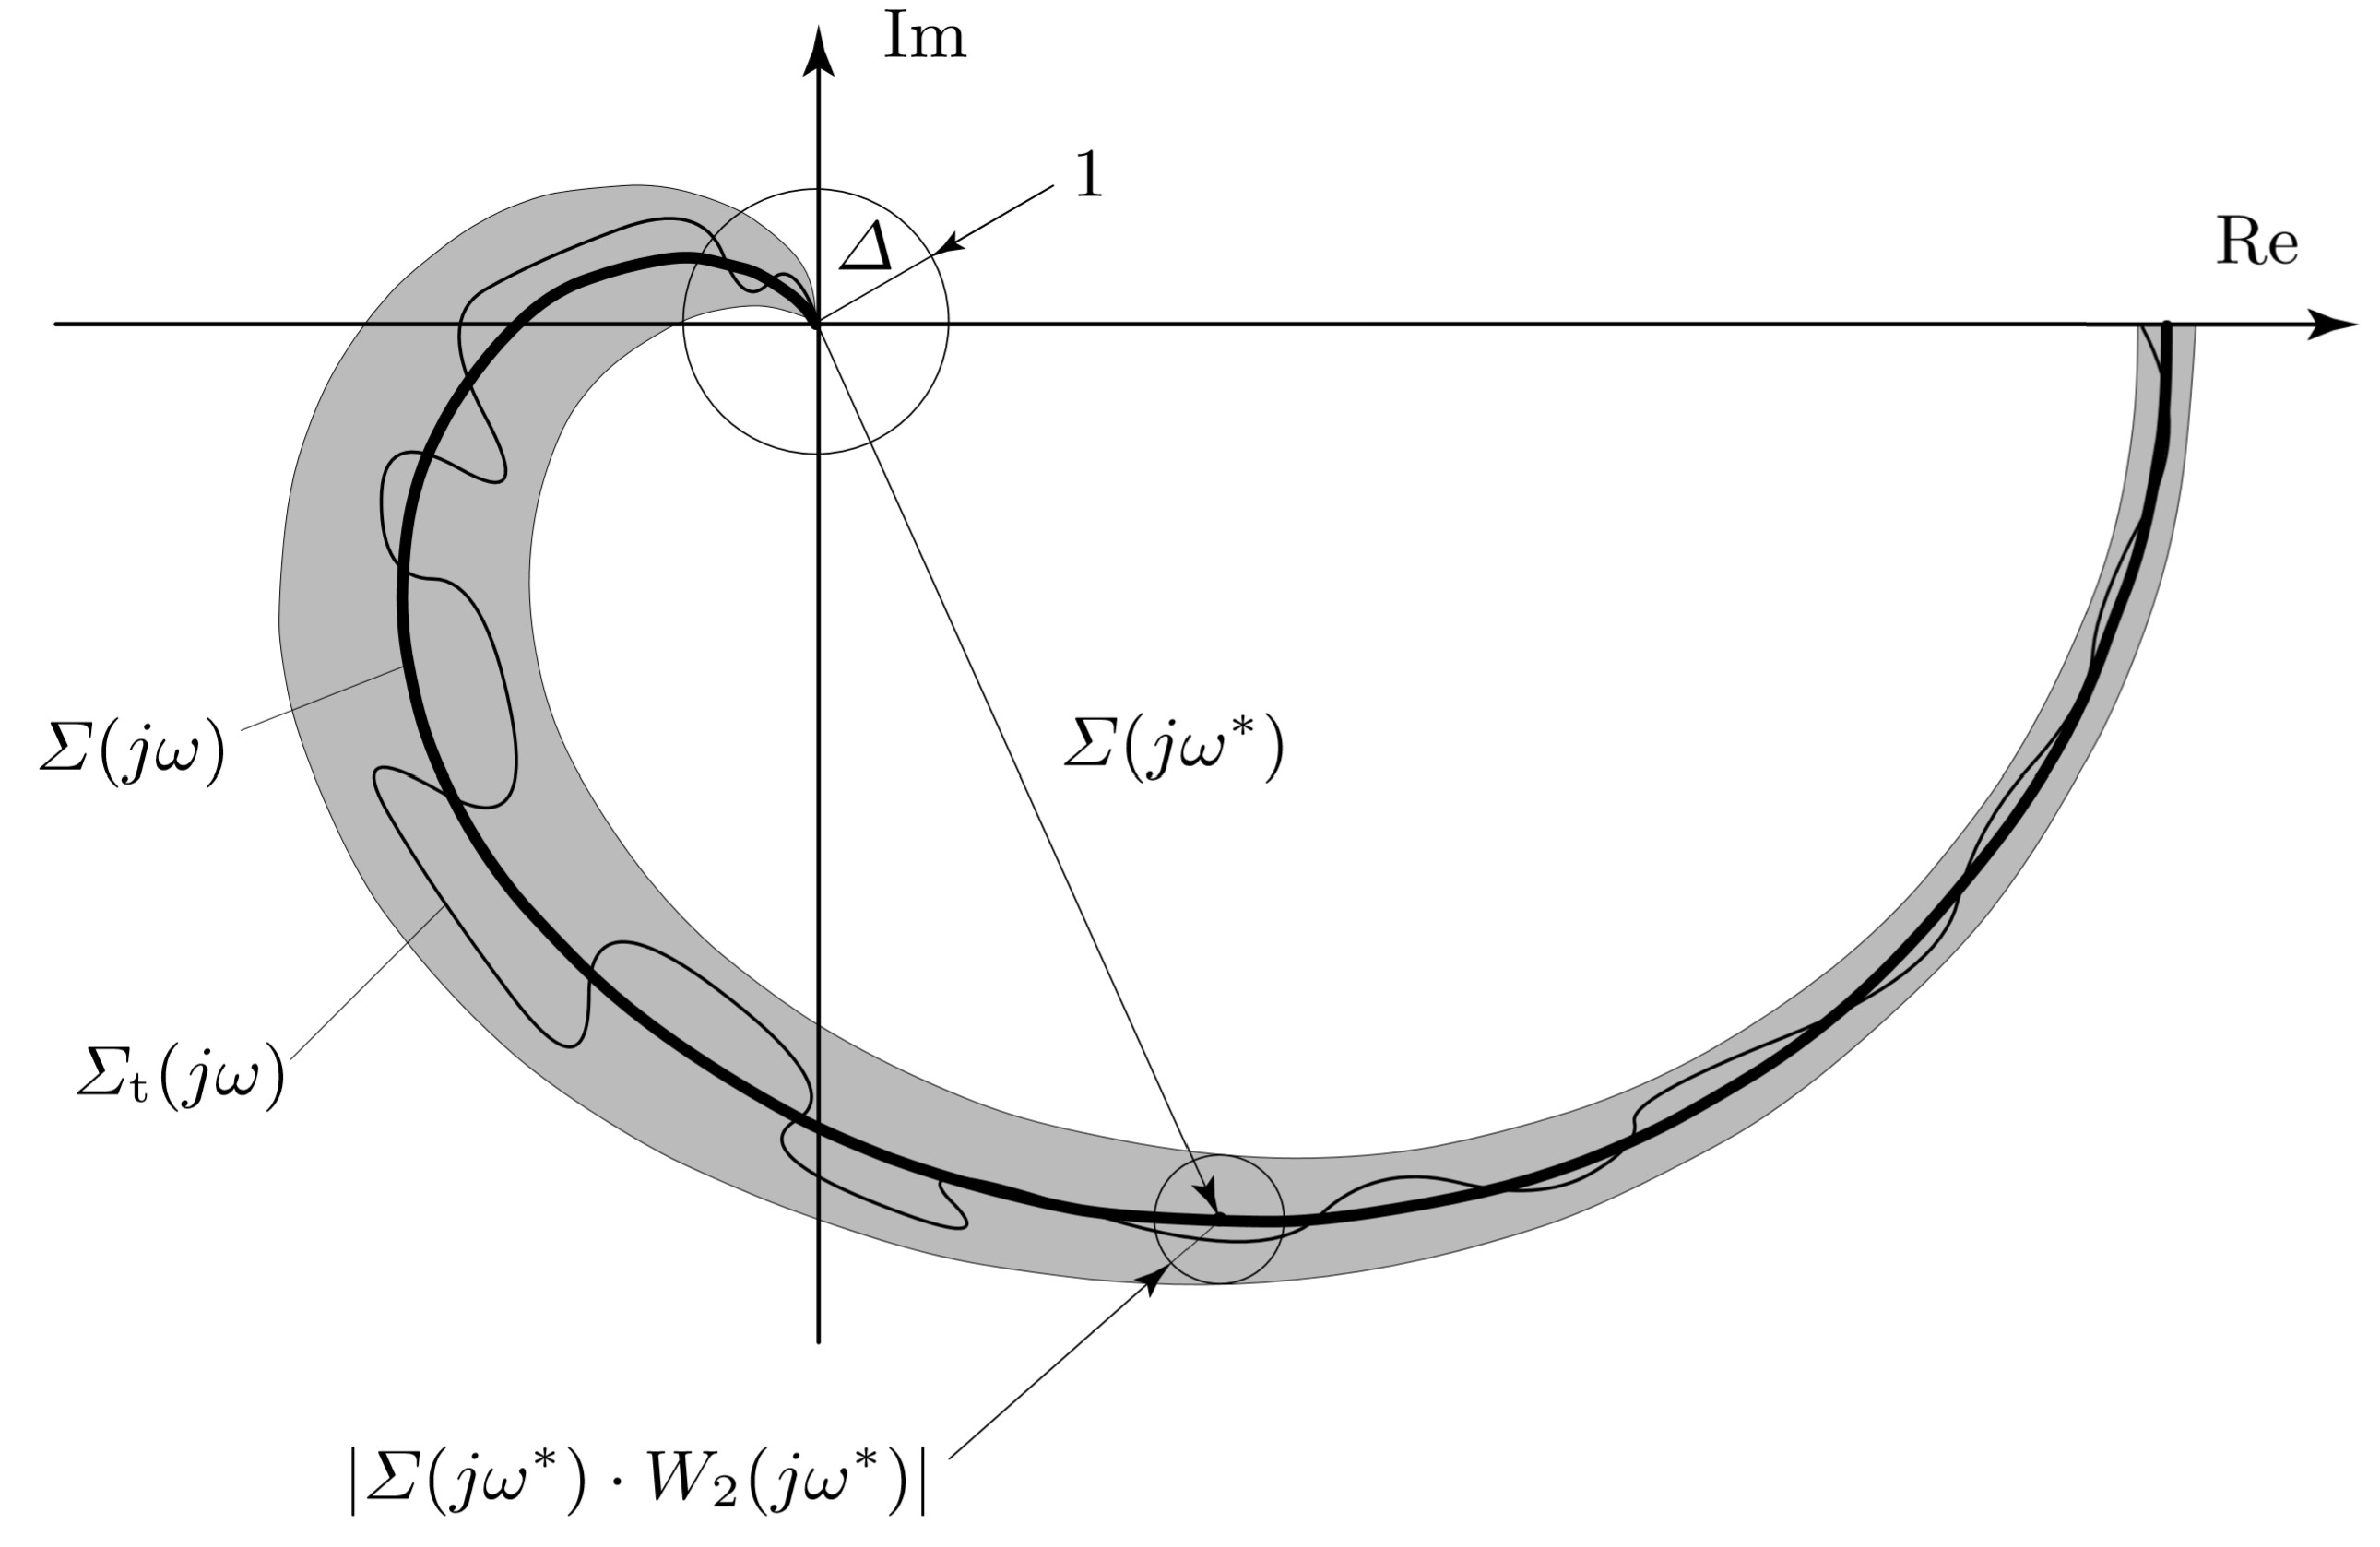
\includegraphics[width = 0.6\linewidth]{images/05/nichtparametrisierte_Unsicherheit.jpg}
            \end{center}
                Annahme: es existiert eine lineare, zeitinvariante wahre Übertragungsfunktion $\Sigma_t(s)$,die das System exakt beschreibt, die jedoch wegen Modellunsicherheiten nicht bekannt ist. Die wahre Übertragungsfunktion $\Sigma(_t(s)$ liegt in der Menge $\mathcal{S}$:
                \[
                \mathcal{S} = \left\{\Sigma(s) \cdot(1+\Delta\cdot W_2(s)) \hspace{3mm} \Delta\begin{cases}  |\Delta| \leq 1\\ \angle \Delta \in[-\pi,\pi]\end{cases}\right\}
                \]
                %alternativ 
                %\mathcal{S} = \{\Sigma(s) \cdot(1+\Delta\cdot W_2(s)) \hspace{3mm} ||\Delta| \leq 1\\ \angle \Delta \in[-\pi,\pi]\}
            
                $\mathbf{\Sigma(S)}$: Nominelle Übertragungsfunktion, durch (imperfekte) Systemodelierung gefunden.
                \\$\mathbf{\Delta}$: Unsicherheitsgenerator: Kreis in der komplexen Ebene.
                \\$\mathbf{W_2(s)}$: Übertragungsfunktion der Unsicherheitsheits: quantifiziert die frequenzabhängige Unsicherheit des Modells
                
                Bei jeder Frequenz $\omega^*$ liegt die wahre Übertragungsfunktion $\Sigma_t(j\omega^*)$innerhalb von einem Kreis mit Radius $|\Sigma(j\omega^*) \cdot W2(j\omega^*|$ um die nominelle Übertragungsfunktion $\Sigma(j\omega^*)$.
            \subsubsection{Unsicherheitsübertragungsfunktion $W_2(s)$}
                Es gibt mehrere Methoden, um ein Modell für die Unsicherheitsübertragungsfunktion zu bestimmen. (Für RT1 ist jedoch nur eine Relevant)
        
               Diese Methode verwendet Messungen am realen System, um die Unsicherheitsgrenzen des Modells davon zu bestimmen:
               
               Vorgehen: 
               \begin{itemize}
                   \item \textbf{Unsicherheitsschätzung mittels Messdaten:}
                   
                   Diese Methode verwendet Messungen am realen System, um die Unsicherheitsgrenzen des Modells davon zu bestimmen.
                \end{itemize}
                   
                   Vorgehen:
                    \begin{enumerate}
                        \item Es werden $k = 1,\hdots,K$ Messungen des Frequenzganges durchgeführt. Für jede Messung bei Frequenz $\omega_i, i =1,\hdots,I$ werden die Werte $|\Sigma(j\omega_{i,k})|$ und $\angle\Sigma(j\omega_{i,k})$ identifiziert.
                        \begin{center}
                            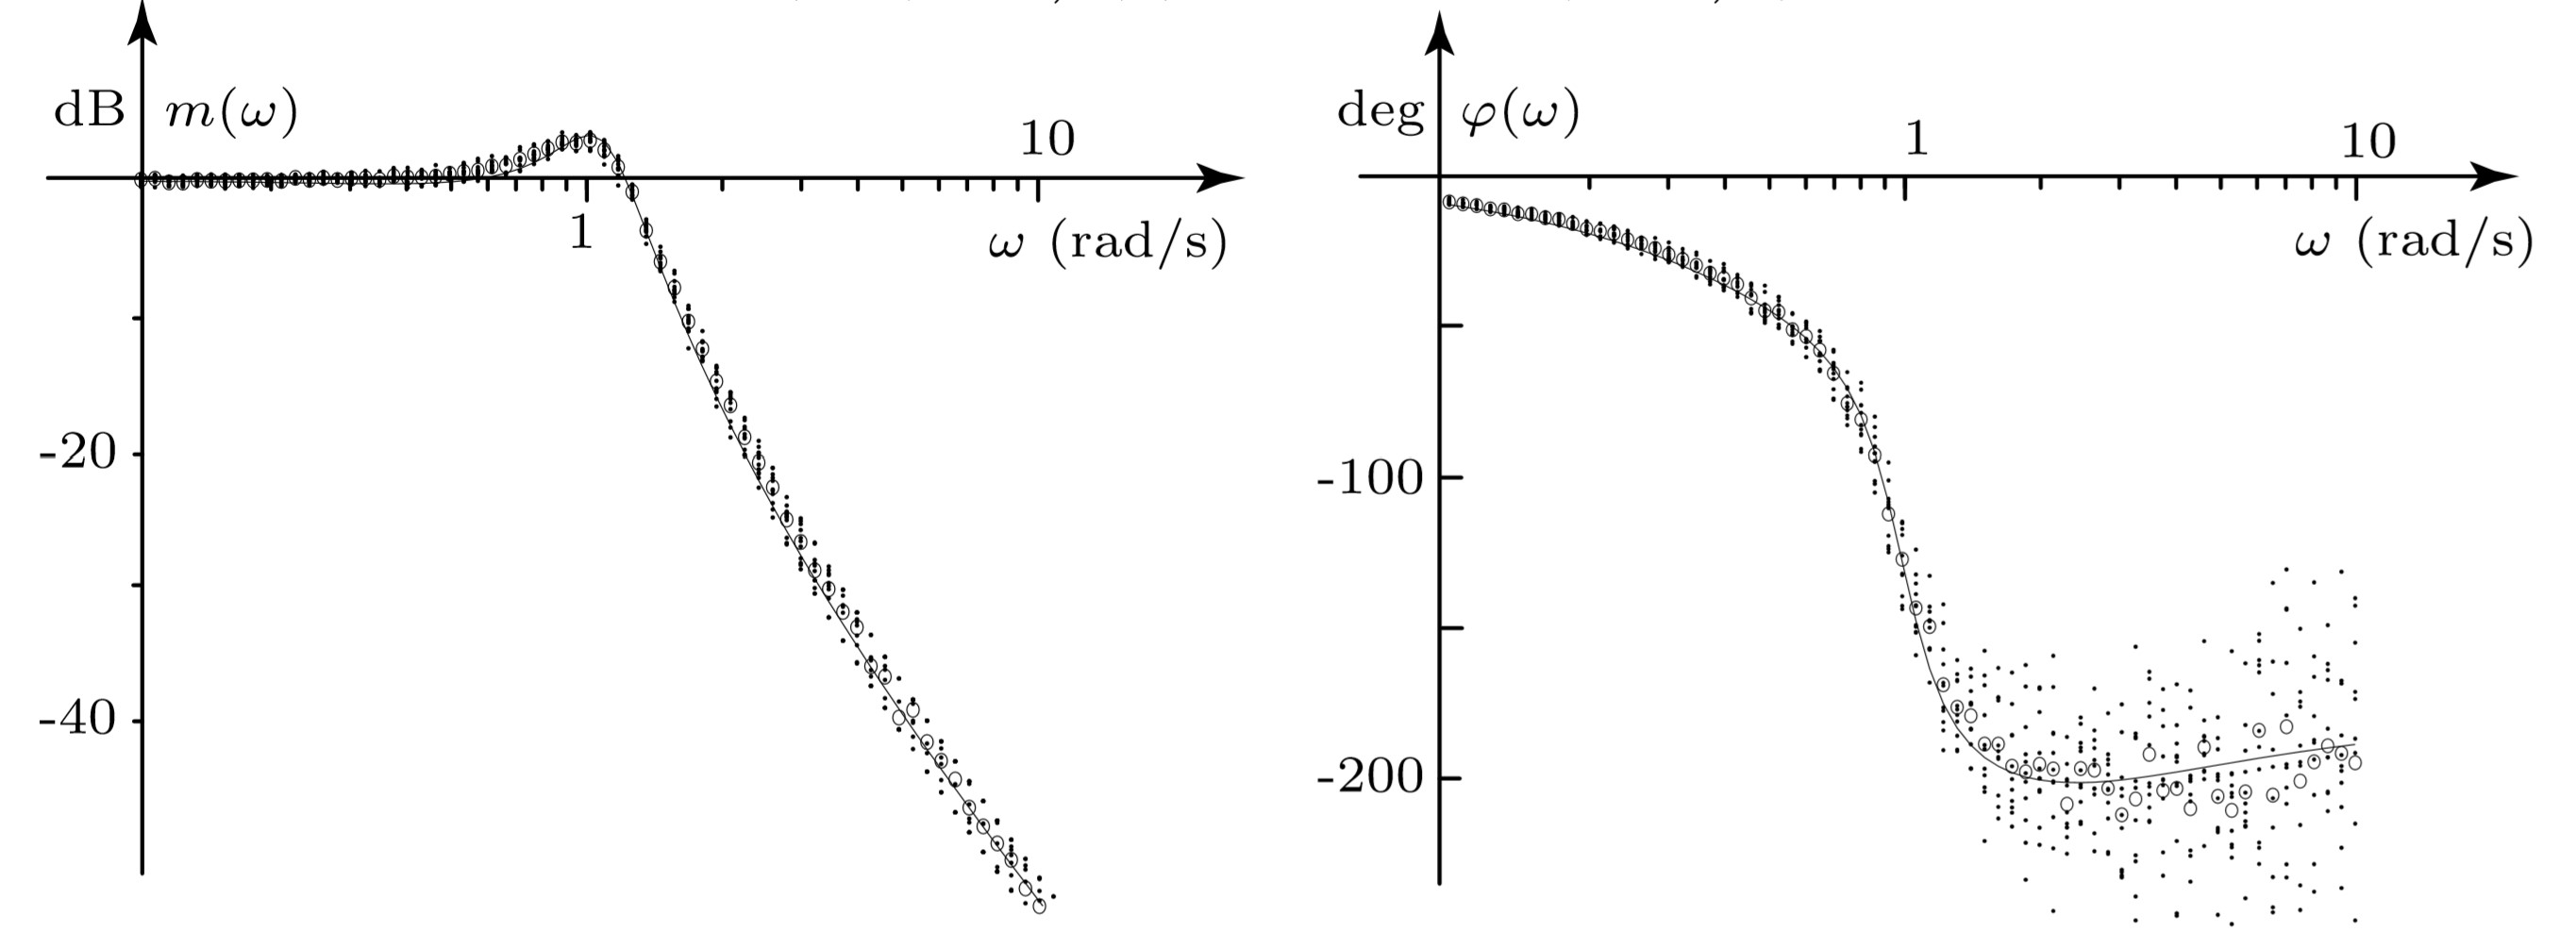
\includegraphics[width = 0.8\linewidth]{images/05/Unsicherheits_Messung.jpg}
                        \end{center}
                        \item Eine nominelle Übertragungsfunktion $\Sigma(s)$ wird an die experimentellen Daten angepasst (analog zur Methode der Systemidentifikation).
                        \[\Sigma(j\omega_i) = m_i \cdot e^{j\cdot\varphi_i}\]
                        \item  Bei jeder Frequenz $\omega_i$ sind die Werte der $K$ Messungen von $|\Sigma(j\omega_{i,k})|$ verteilt um den Wert der nominellen Übertragungsfunktion $|\Sigma(j\omega_i)|$. Die Unsicherheitsübertragungsfunktion bildet einen Kreis mit Radius $|W_2(j\omega_i)|$ um $|\Sigma(j\omega_i)|$ so dass alle Messpunkte von $|\Sigma(j\omega_{i,k})|$ darin enthalten sind:
                        \[\frac{\Sigma(j\omega_{i,k})}{\Sigma(j\omega_i)}-1 < |W_2(j\omega_i)|k\in [1,K] i \in[1,I]\]
                        
                        Die Ungleichung definiert eine Bedingung bei jeder Frequenz $\omega_i$. Wird die Linke Seite der Ungleichung als Funktion der Frequenz dargestellt, ergibt sich:
                        \begin{center}
                            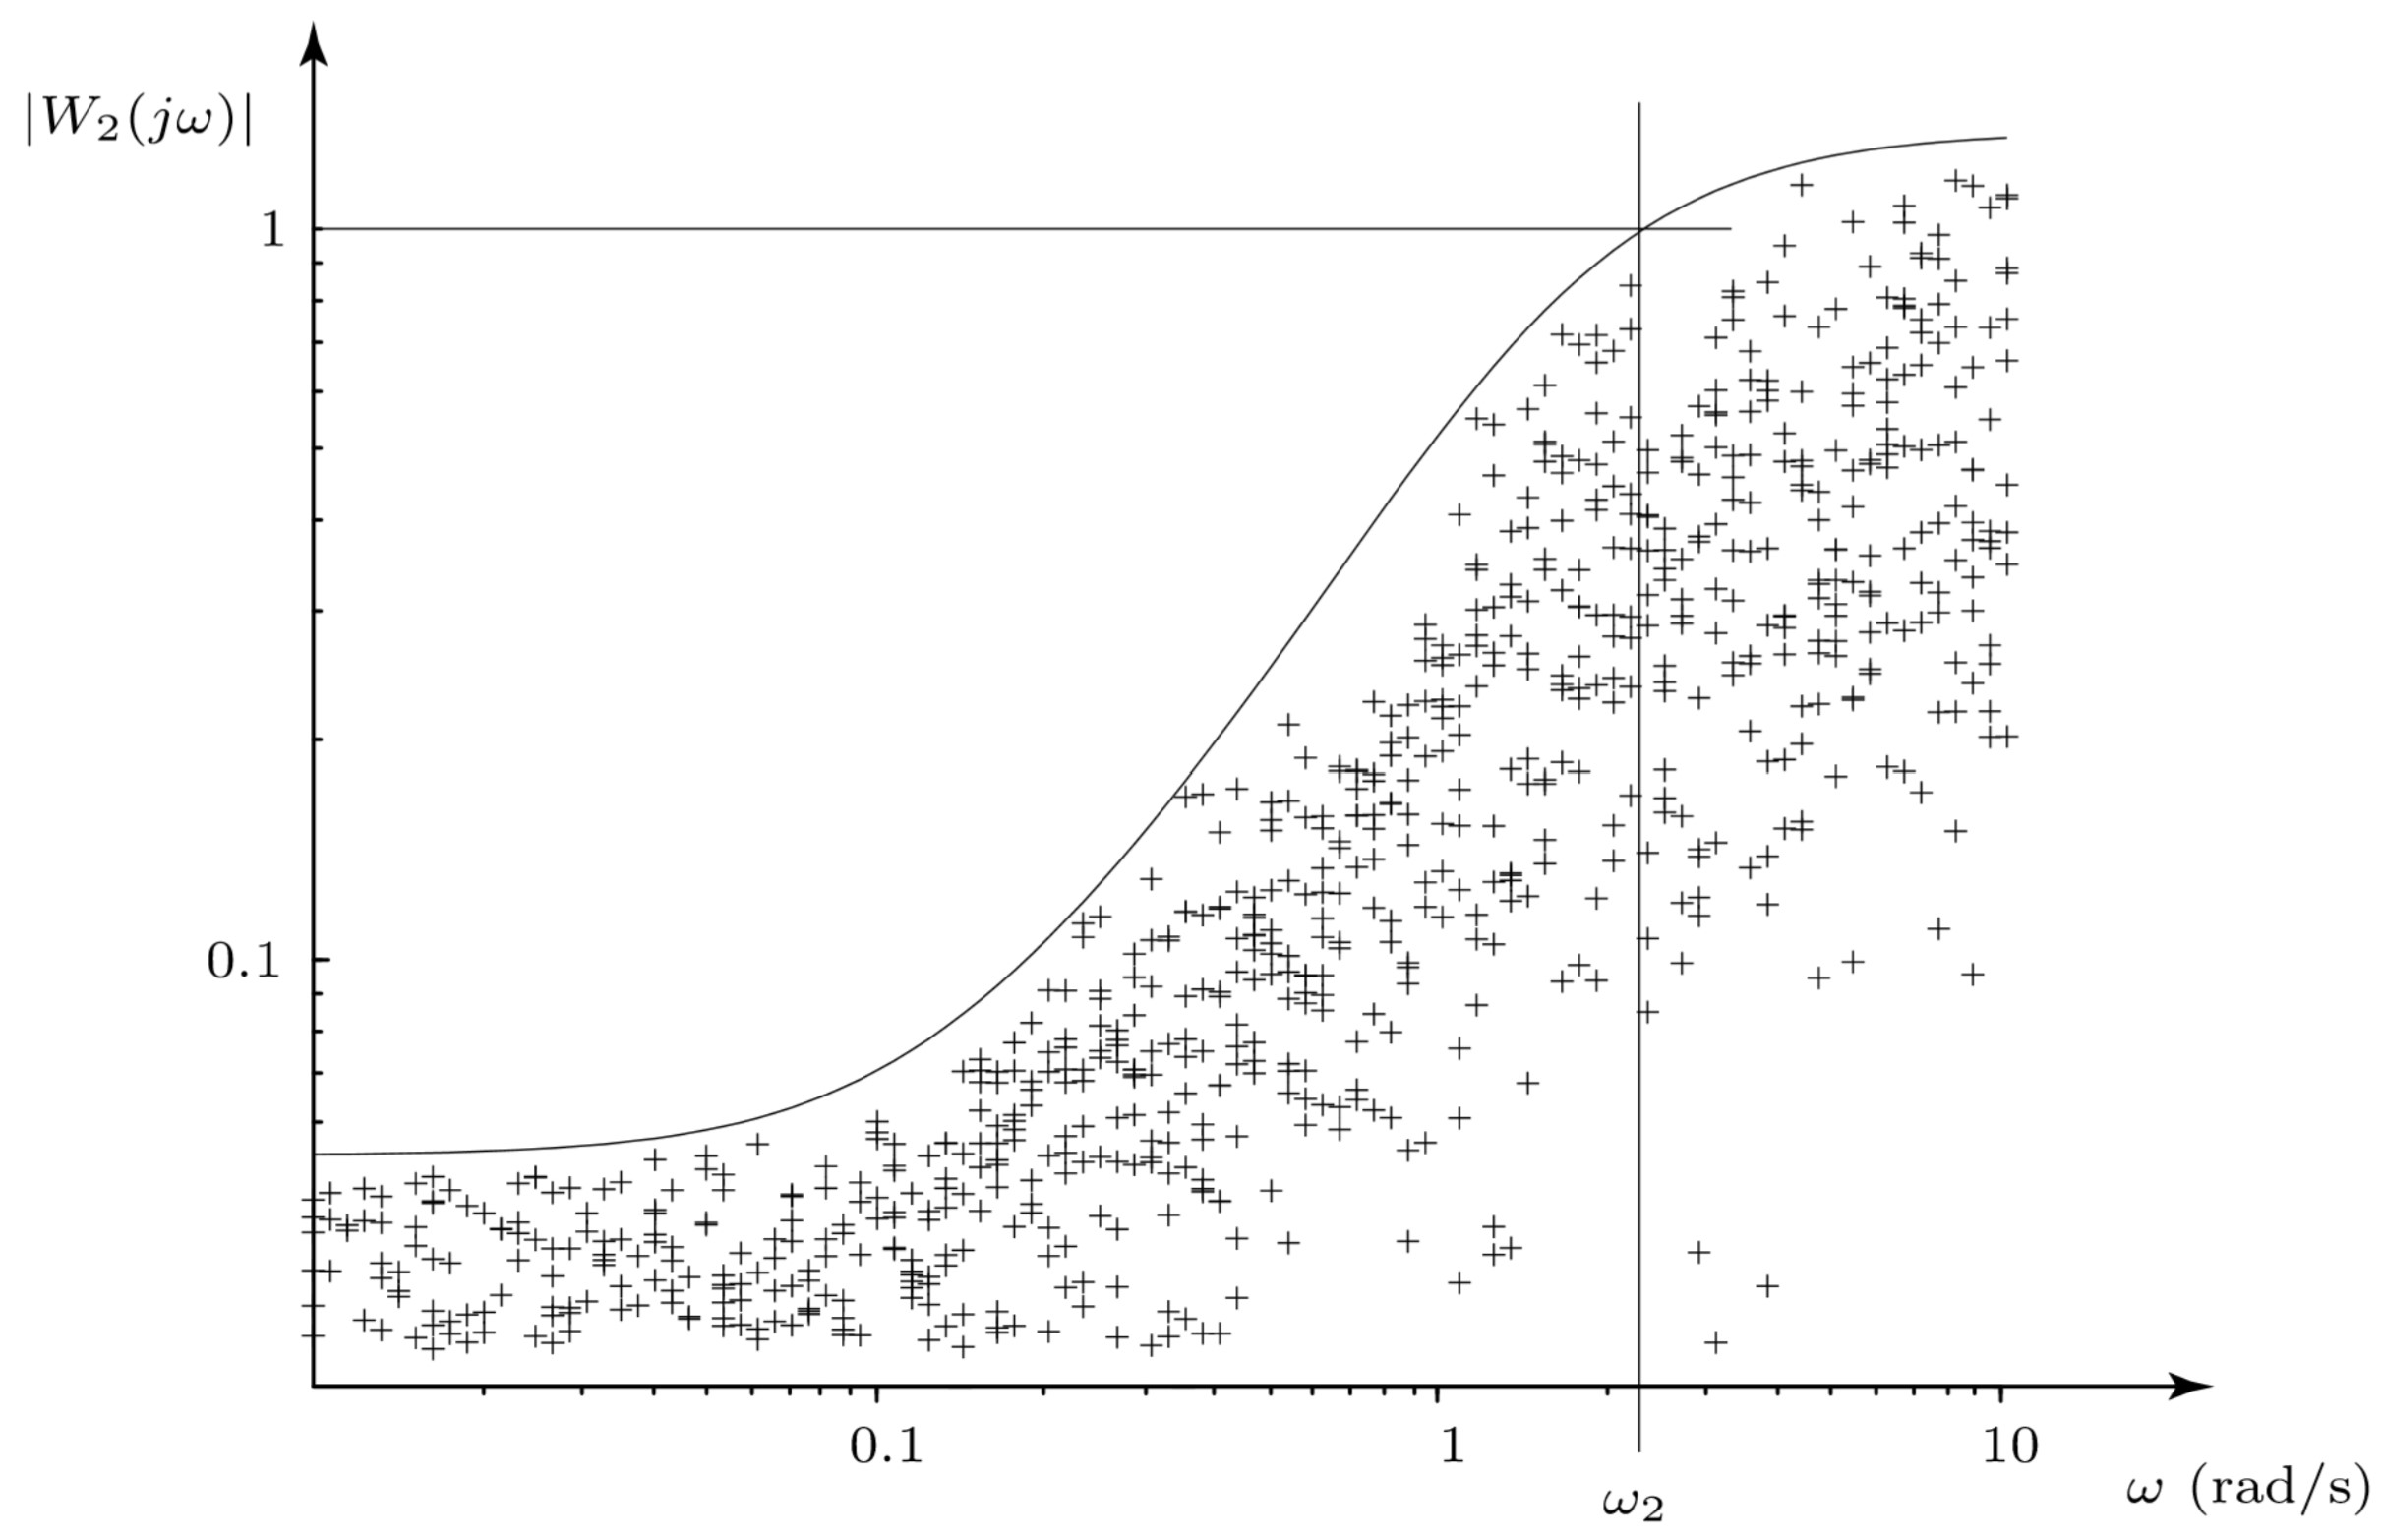
\includegraphics[width = 0.65\linewidth]{images/05/UnsicherheitsFunktion.jpg}
                        \end{center}
                        \textbf{Bemerkungen:} 
                        
                        Die Unsicherheit steigt bei höheren Frequenzen, den Daten kann eine Unsicherheitsübertragungsfunktion $W_2(s)$ zugeordnet werden.
                        
                        Die Unsicherheitsübertragungsfunktion $W_2(s)$ enthält keine Phaseninformation.
                        

                    \end{enumerate}
                    %nicht relevant für RT1
                    % \item\textbf{approximation durch varieren der Parameter}
                    
                    % Eine Mathemathische Greybox-model wurde ermittelt und alle Parameter sind bekannt und liegen in bestimmten Intervallen.
                    
                    % \begin{enumerate}
                    %     \item Mit diesen Daten kann ein groben Ansatz gemacht werden, bei dem die Parameter-Intervalle im finiten Gitter abgedeckt ("covered" - geplotted?) werden und dann in einem zweiten Schritt die Frequenzantwort von allen Gitter Punkten berechnet wird.
                    %     \item Weiter vorgehen wie bei \textit{Unsicherheitsschätzung mittels Messdaten}
                    % \end{enumerate}
                    % \item\textbf{Unsicherheit durch simplifiziertes Modell:}
                    % Ein mathematisches Modell von einer Strecke ist bekannt, jedoch zu komplex für das designen eines Kontrollsystems. Ziel ist es das Modell mit einem simpleren Modell in Kombination mit einer Unsicherheitsschranke zu approximieren, welche das ursprüngliche komplexe Modell beinhaltet
 \section{Systemidentifikation}
    \subsection{Modelle}
        In der Regelungstechnik arbeitet man mit verschiedenen Modellen. Generell unterscheidet man zwischen folgenden drei Arten.
        \subsubsection{White Box model} 
         \begin{wrapfigure}[5]{r}{0.4\linewidth}
                \vspace{-6mm}
                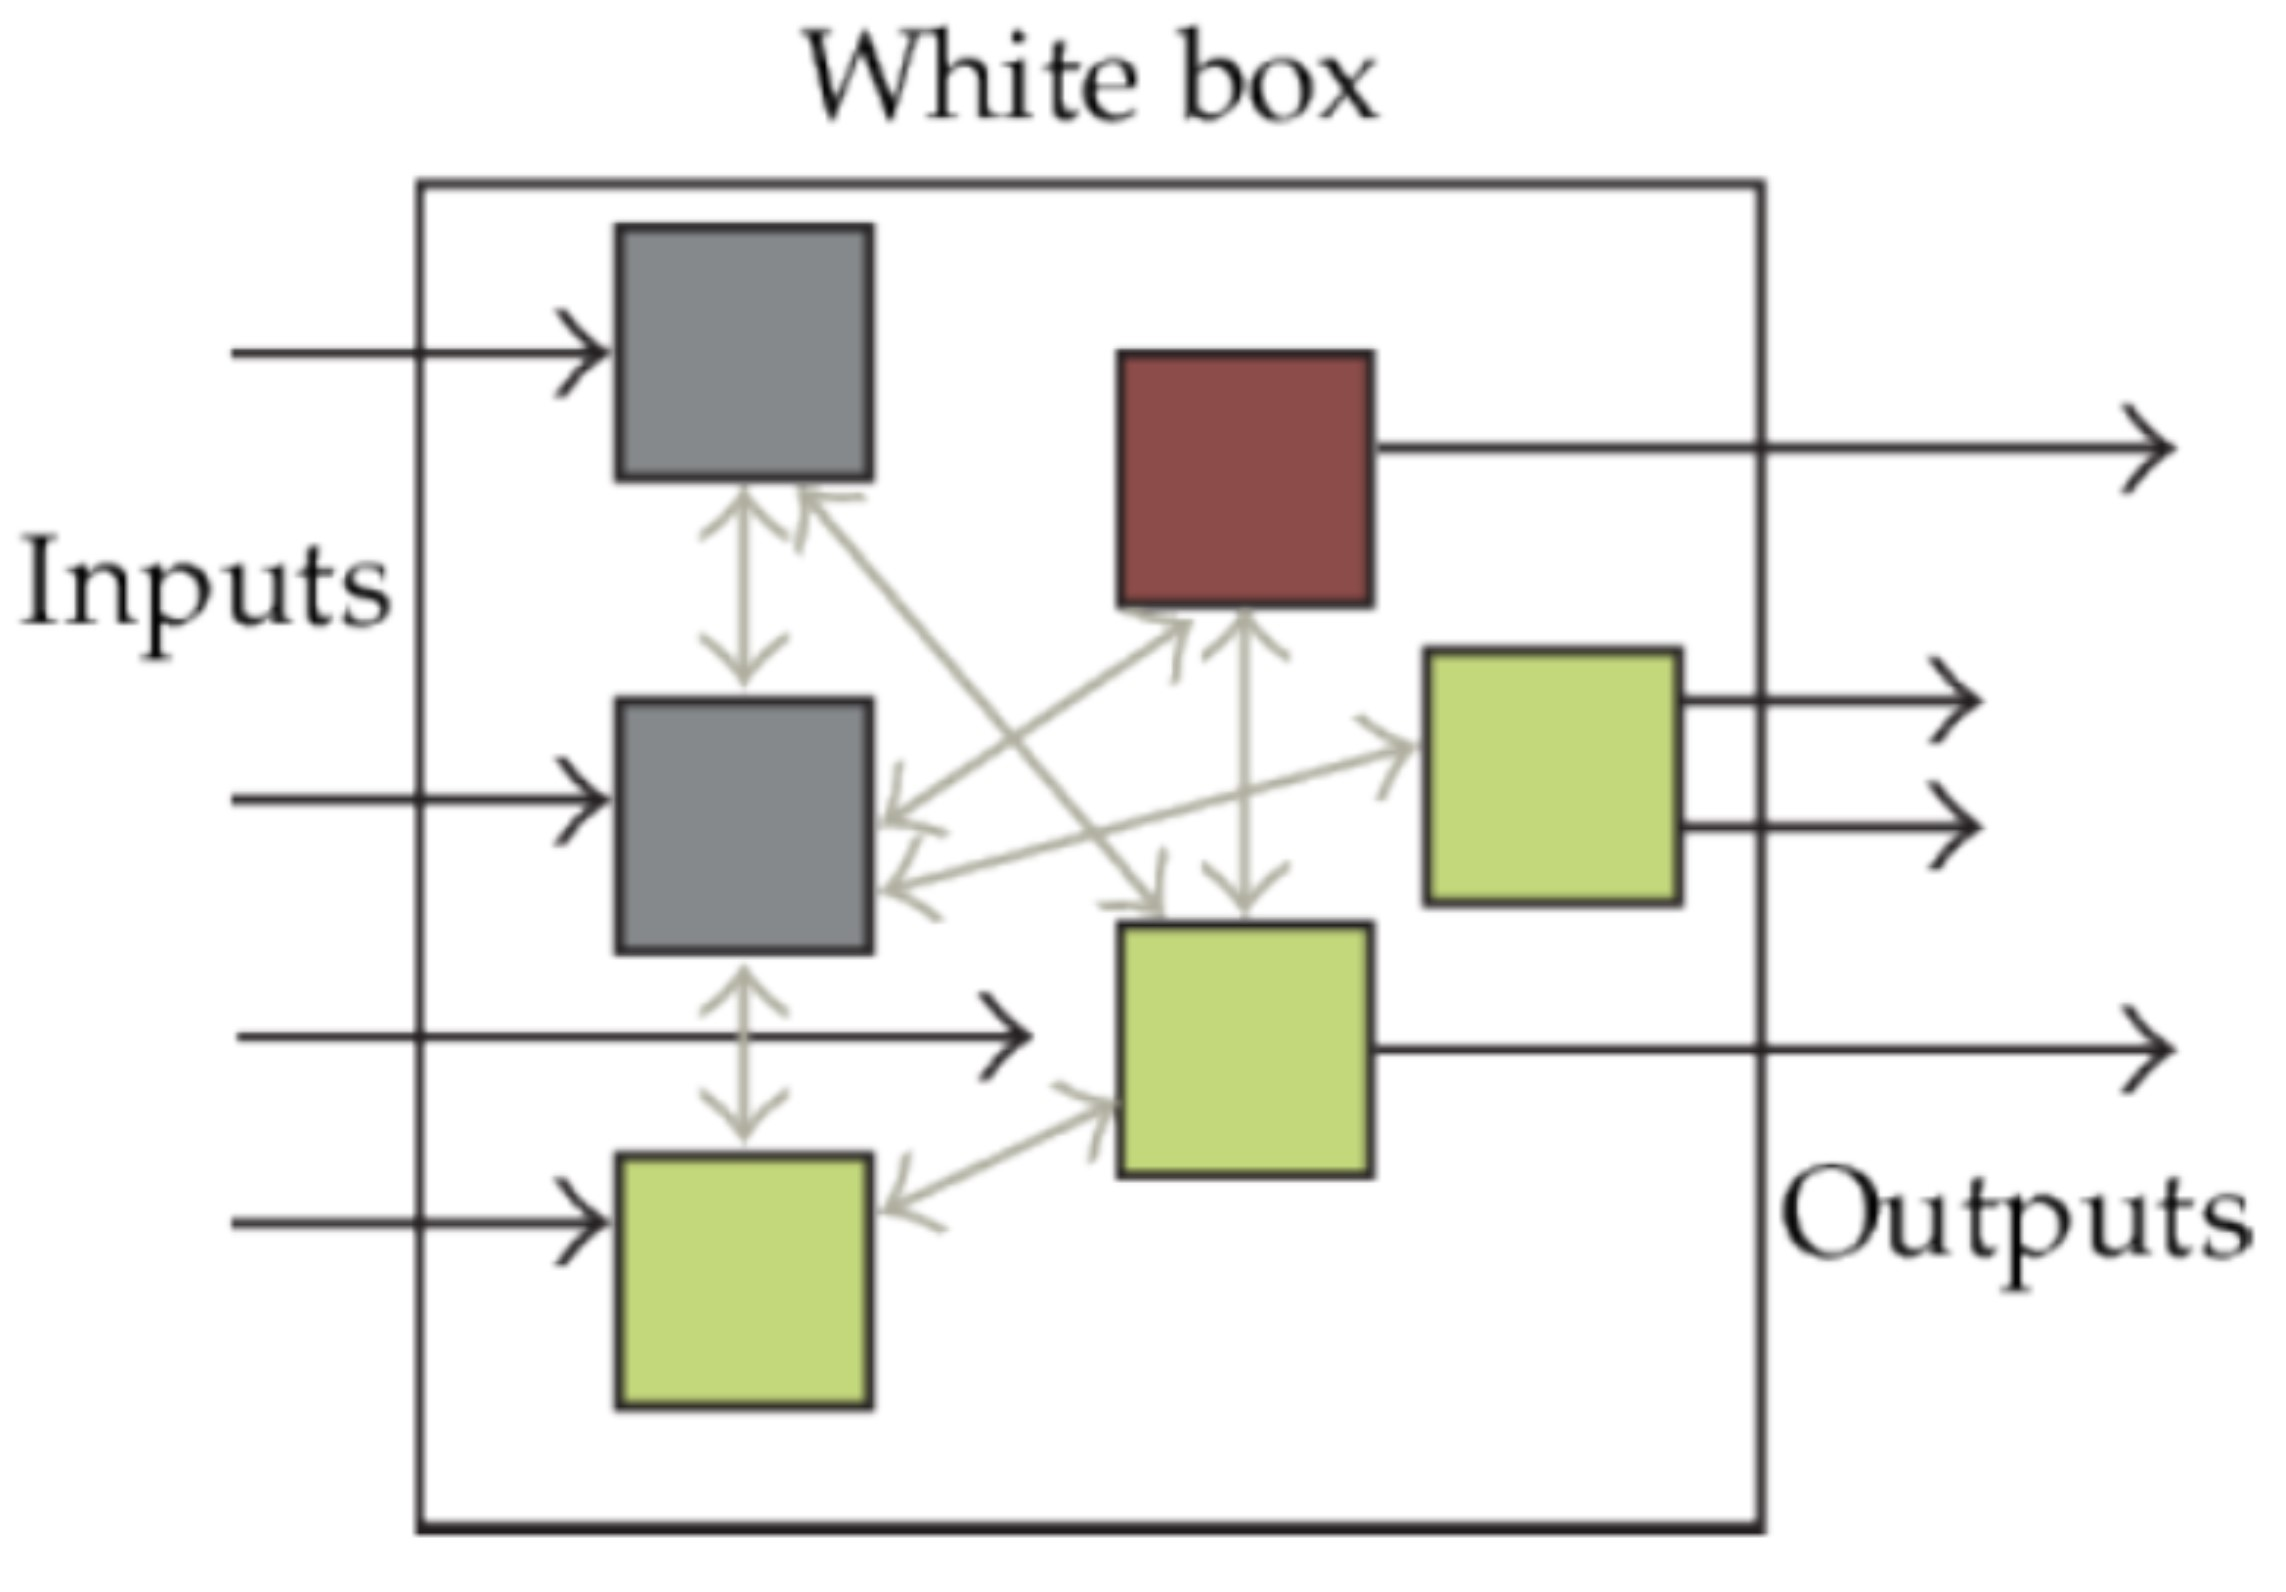
\includegraphics[width=\linewidth]{images/06/Whitebox.jpg}
            \end{wrapfigure}
            Es existiert eine Explizite Darstellung der Physik des Systems mit bekannten Parameterwerten.Das Verhalten, die Werte und der Zusammenhang zwischen den Zuständen ist vollständig bekannt.
        \subsubsection{Grey Box model}
            \begin{wrapfigure}[5]{r}{0.35\linewidth}
                \vspace{-6mm}
                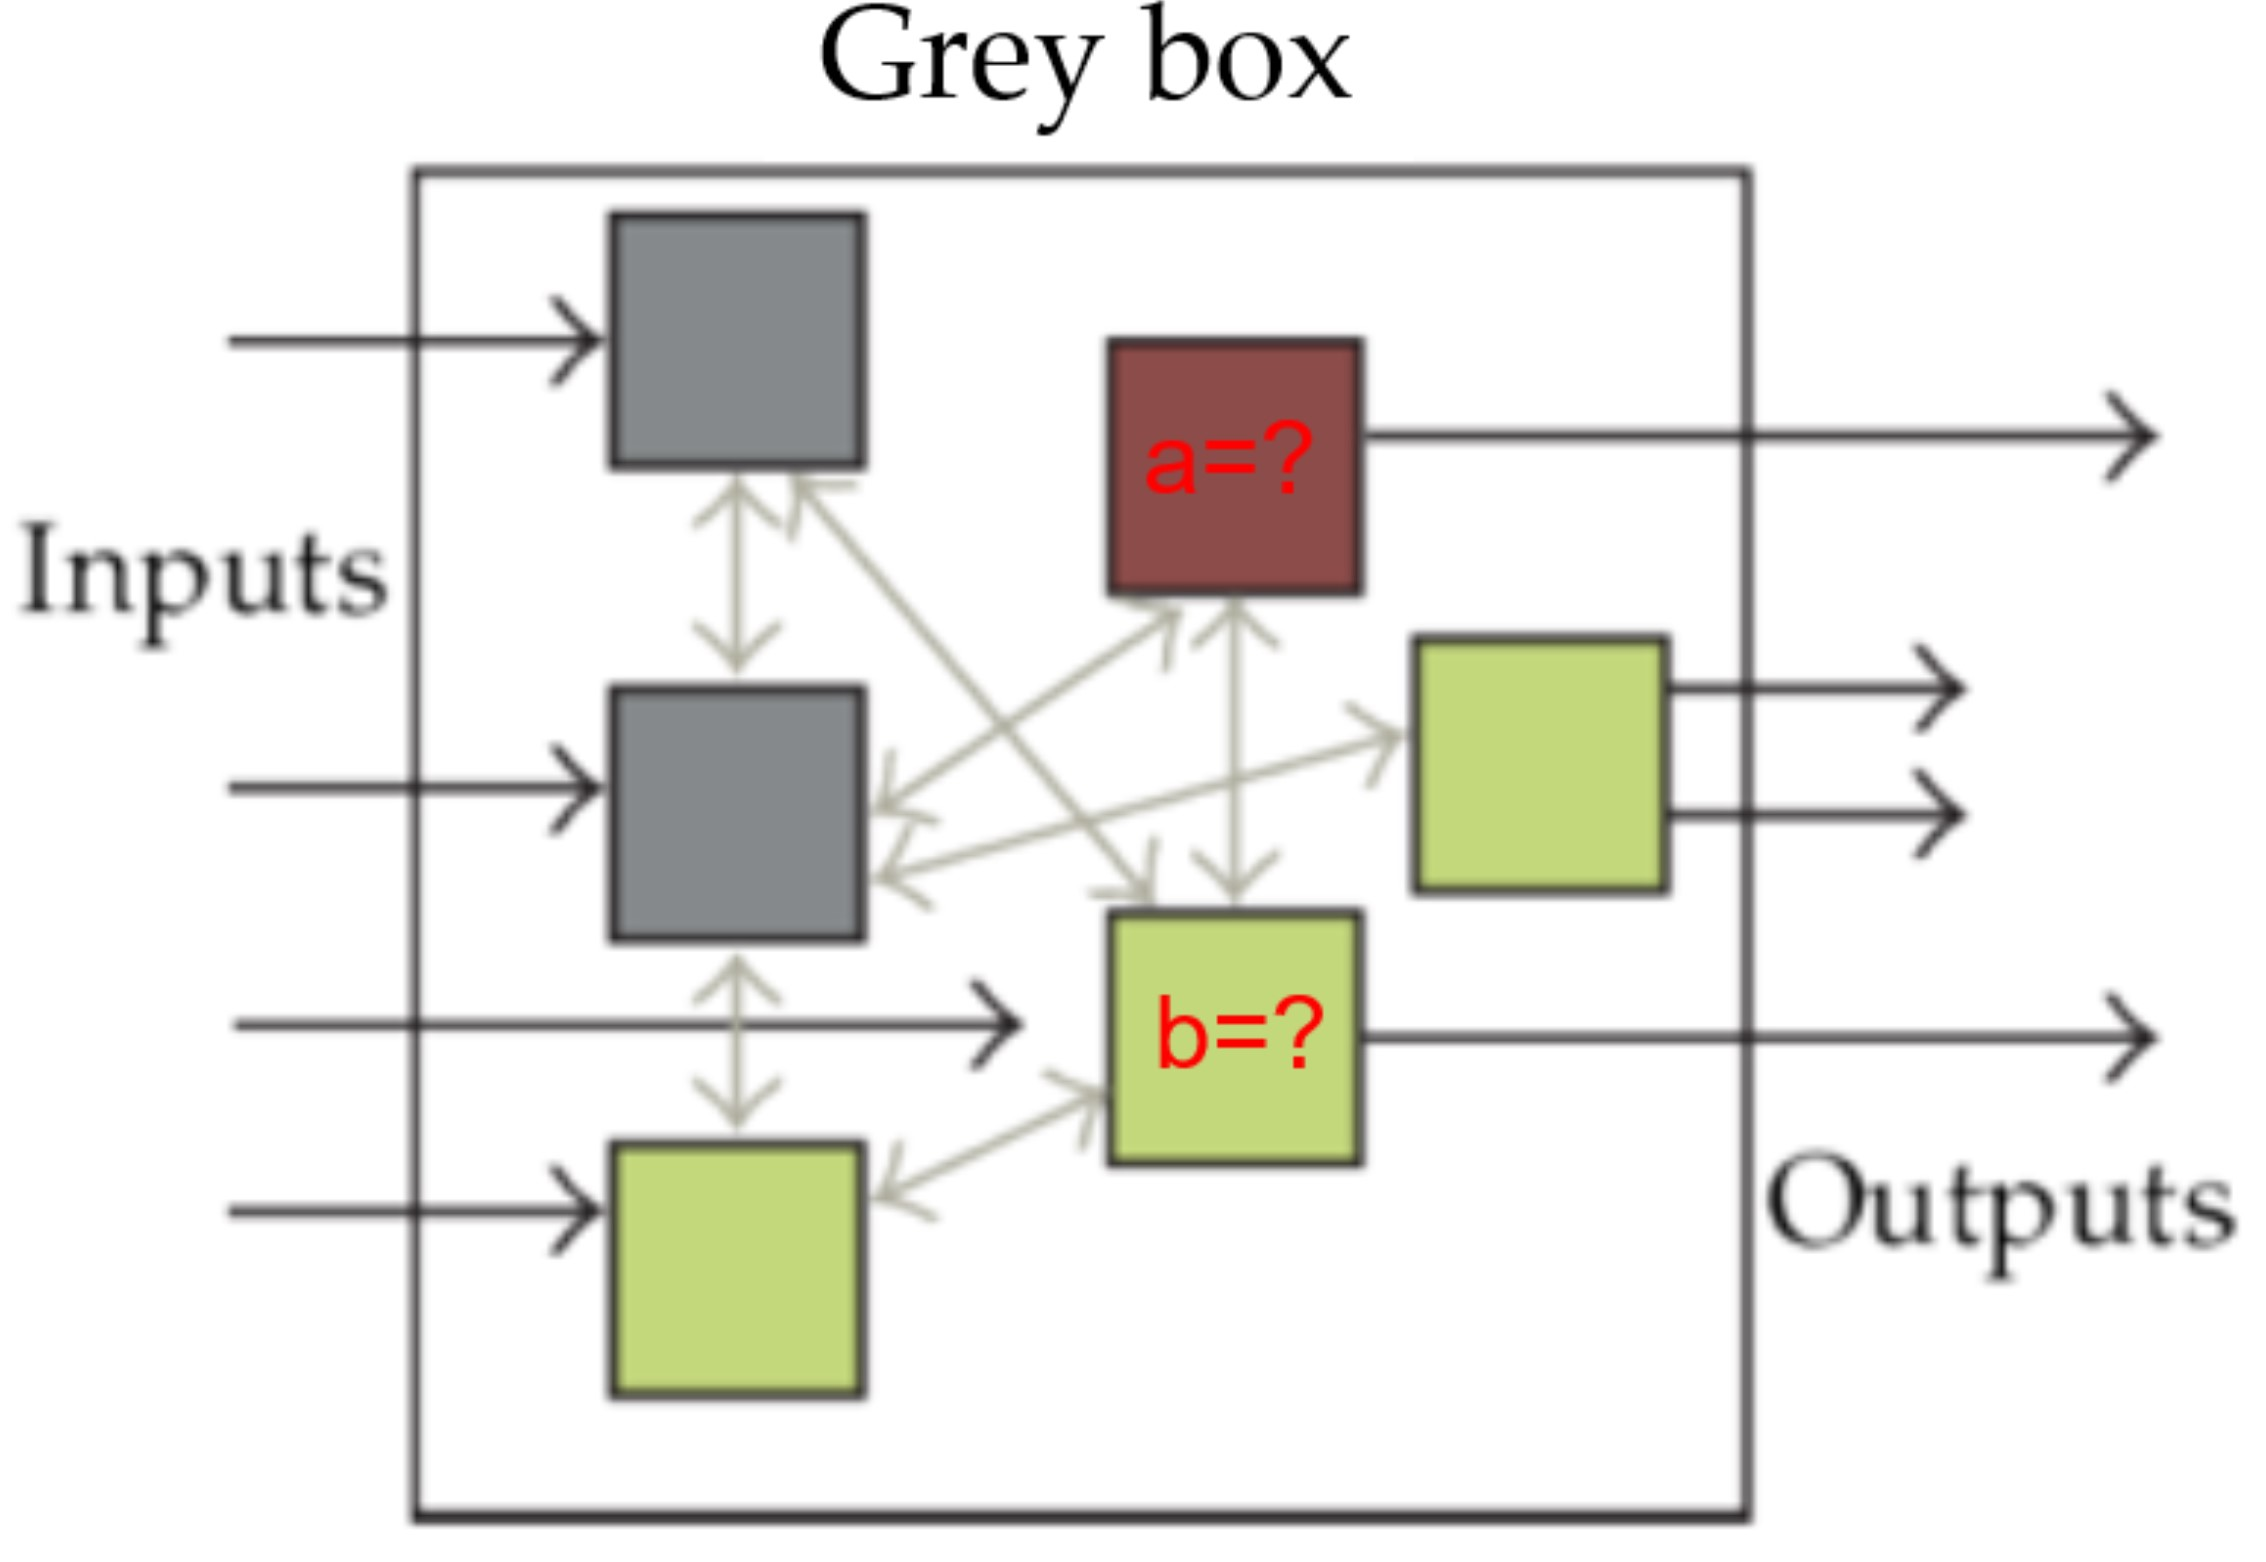
\includegraphics[width=\linewidth]{images/06/Greybox.jpg}
            \end{wrapfigure}
            Es existiert eine explizite Darstellung der Physik des Systems mit \textit{unbekannten} Parameterwerten. Die Zusammenhänge und Verhalten der Zustände sind jedoch bekannt.\\
            
            
           
        \subsubsection{Black Box model}
            \begin{wrapfigure}[4]{r}{0.3\linewidth}
                \vspace{-6mm}
                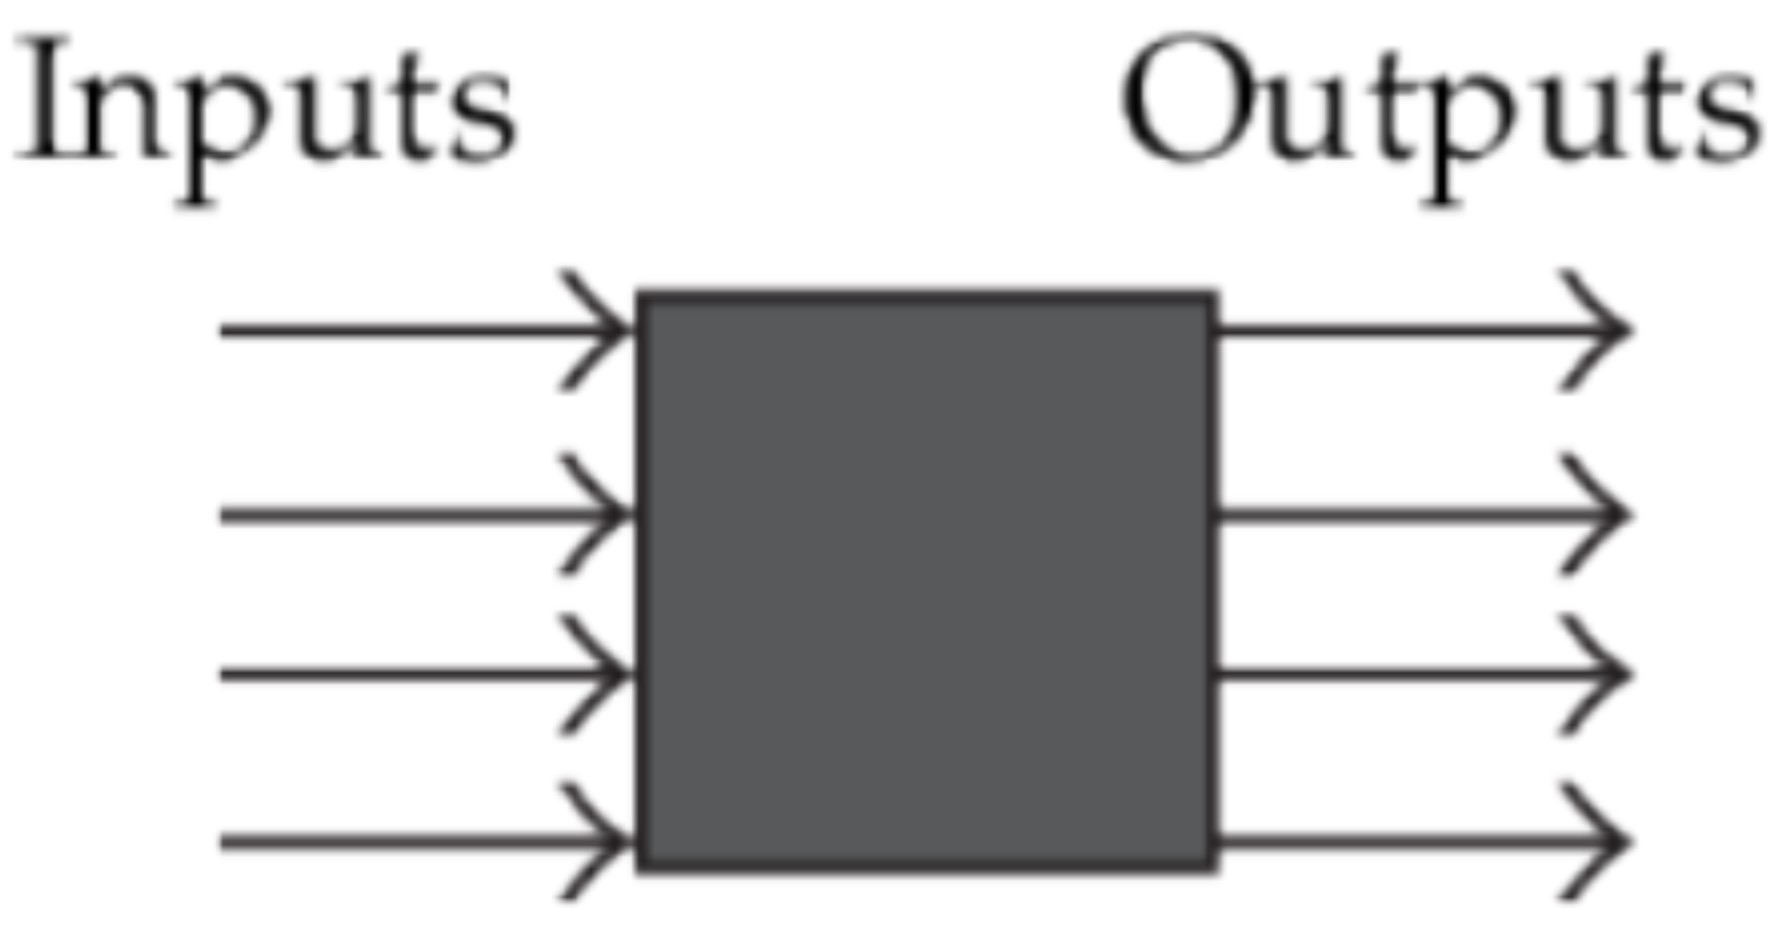
\includegraphics[width=\linewidth]{images/06/Blackbox.jpg}
            \end{wrapfigure}
            Es existiert keine explizite Darstellung der Physik des Systems. Das Systemverhalten muss durch empirische Datenanalyse ermittelt werden. 
           
            Black box Modelle werden verwendet wenn die Physik des Systems nicht genau bekannt oder zu komplex ist um einfach modelliert zu werden. Durch experimentelle Modellbildung (Systemidentifikation) kann ein Modell des Systems abgeleitet werden, das für die Reglerentwicklung erforderlich ist. 
            
        \subsubsection{Systemidentifikation mittels Frequenzgang}
            Ein unbekanntes System kann wie folgt identifiziert werden:
            \begin{enumerate}
                \item Das System wird mit einem bekannten harmonischen Eingangssignal angeregt: $u(t) = cos(\omega t),\omega \in [0,\infty).$
                \item Die Verstärkung $|\Sigma(j\omega)|$ und die Phase $\angle\Sigma(j\omega)$ der Systemantwort $y_\infty = |\Sigma(j\omega)| \cdot cos(\omega t + \angle\Sigma(j\omega))$ werden gemessen. Somit kann das Bodediagramm des Systems experimentell bestimmt werden.
                \item Eine Übertragungsfunktion wird an die Daten angepasst. Hier ist es wichtig, die Auswirkung verschiedener Standardelementen auf Magnitude und Phase zu verstehen.
            \end{enumerate}
\section{Analyse von Regelsystemen}
    \subsection{Signale im Regelkreis}
    \begin{tabular}{l|l}
    $\mathbf{r(t)}$& Referenz (Sollzustand des Systems)\\
    $\mathbf{w(t)}$& Störung der Eingangsgrösse $u$\\
    $\mathbf{d(t)}$& Störung der Ausgangsgrösse $y$\\
    $\mathbf{n(t)}$& Sensorrauschen\\
    $\mathbf{e(t)}$& Regelfehler\\
    $\mathbf{y(t)}$& Ist-Wert/Ausgangsgrösse\\
    $\mathbf{u(t)}$& Stellgrösse\\
    \end{tabular}
    
    \begin{center}
        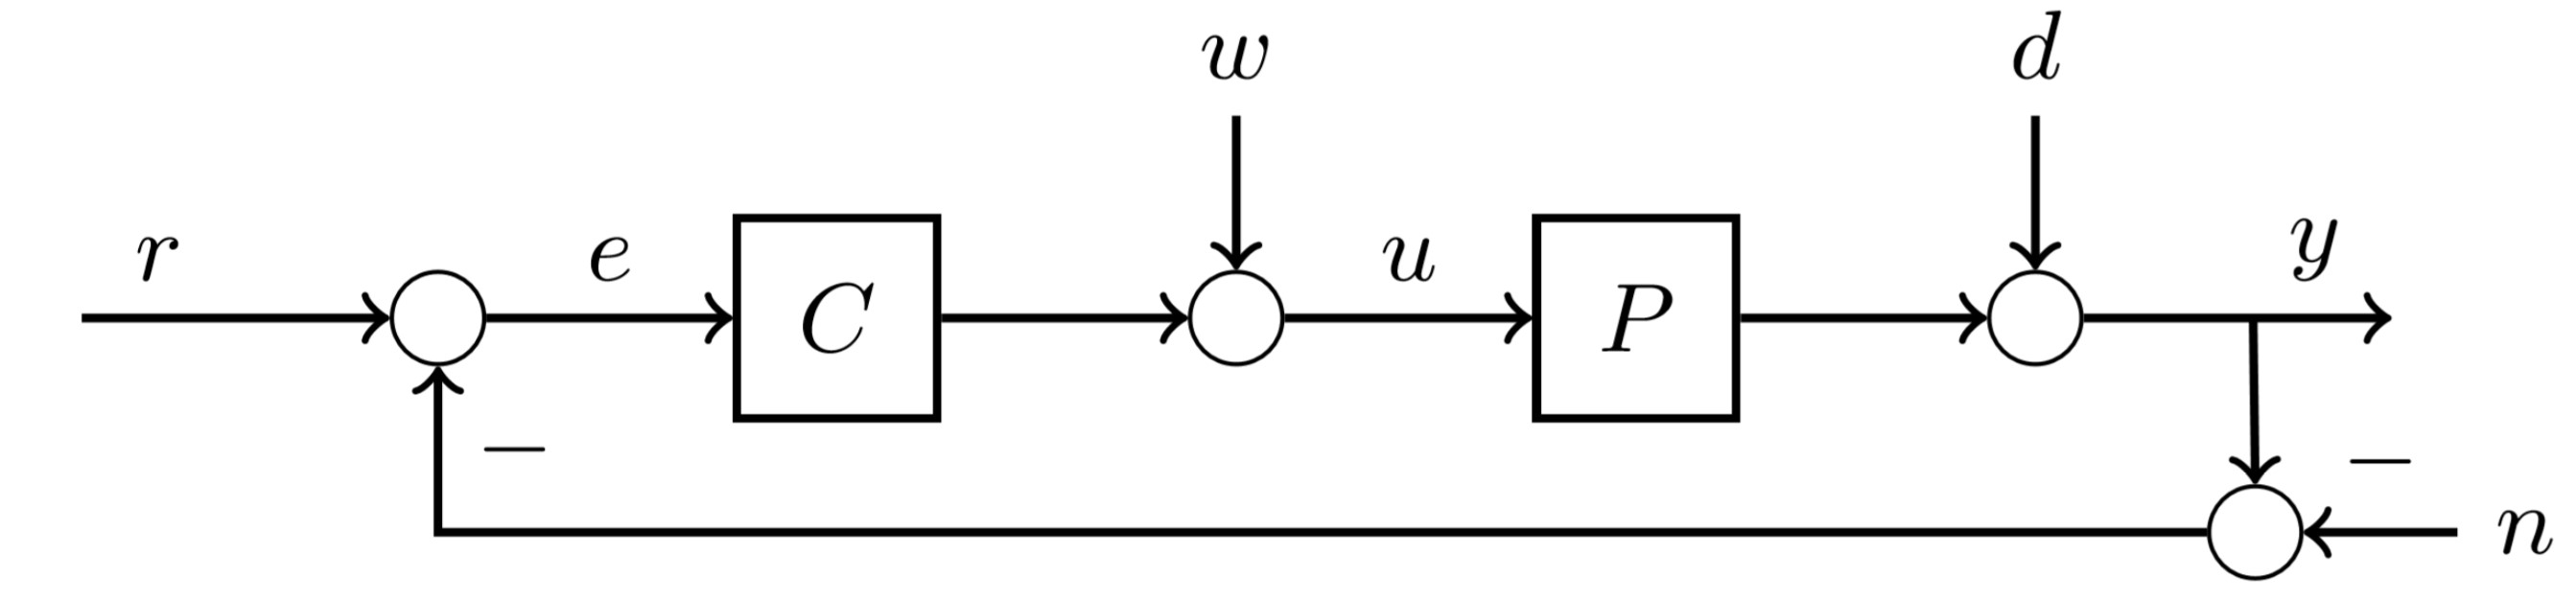
\includegraphics[width = 0.8\linewidth]{07/Standart_Regelkreis.jpg}
    \end{center}
    
    Um die Beziehung zwischen zwei beliebigen Signalen zu beschreiben. wird der Regelkreis zuerst in den Frequenzbereich transformiert:

    \begin{center}
        \includegraphics[width = 0.8\linewidth]{images/07/Standart_Regelkreis_FB.jpg}
    \end{center}
    
    Dabei soll die \textbf{Ausgangsgrösse} $Y(s)$ als Funktion des \textbf{Reglers} $C(s)$, der \textbf{Regelstrecke} $P(s)$ und der \textbf{Eingänge} $R(s)$, $N(s)$, $D(s)$, und $W(s)$ geschrieben werden.
    Durch die Linearität der Regelstruktur und Annahme von unkorrelierten Eingängen können die Eingangsbeiträge einzeln betrachtet werden.
    
    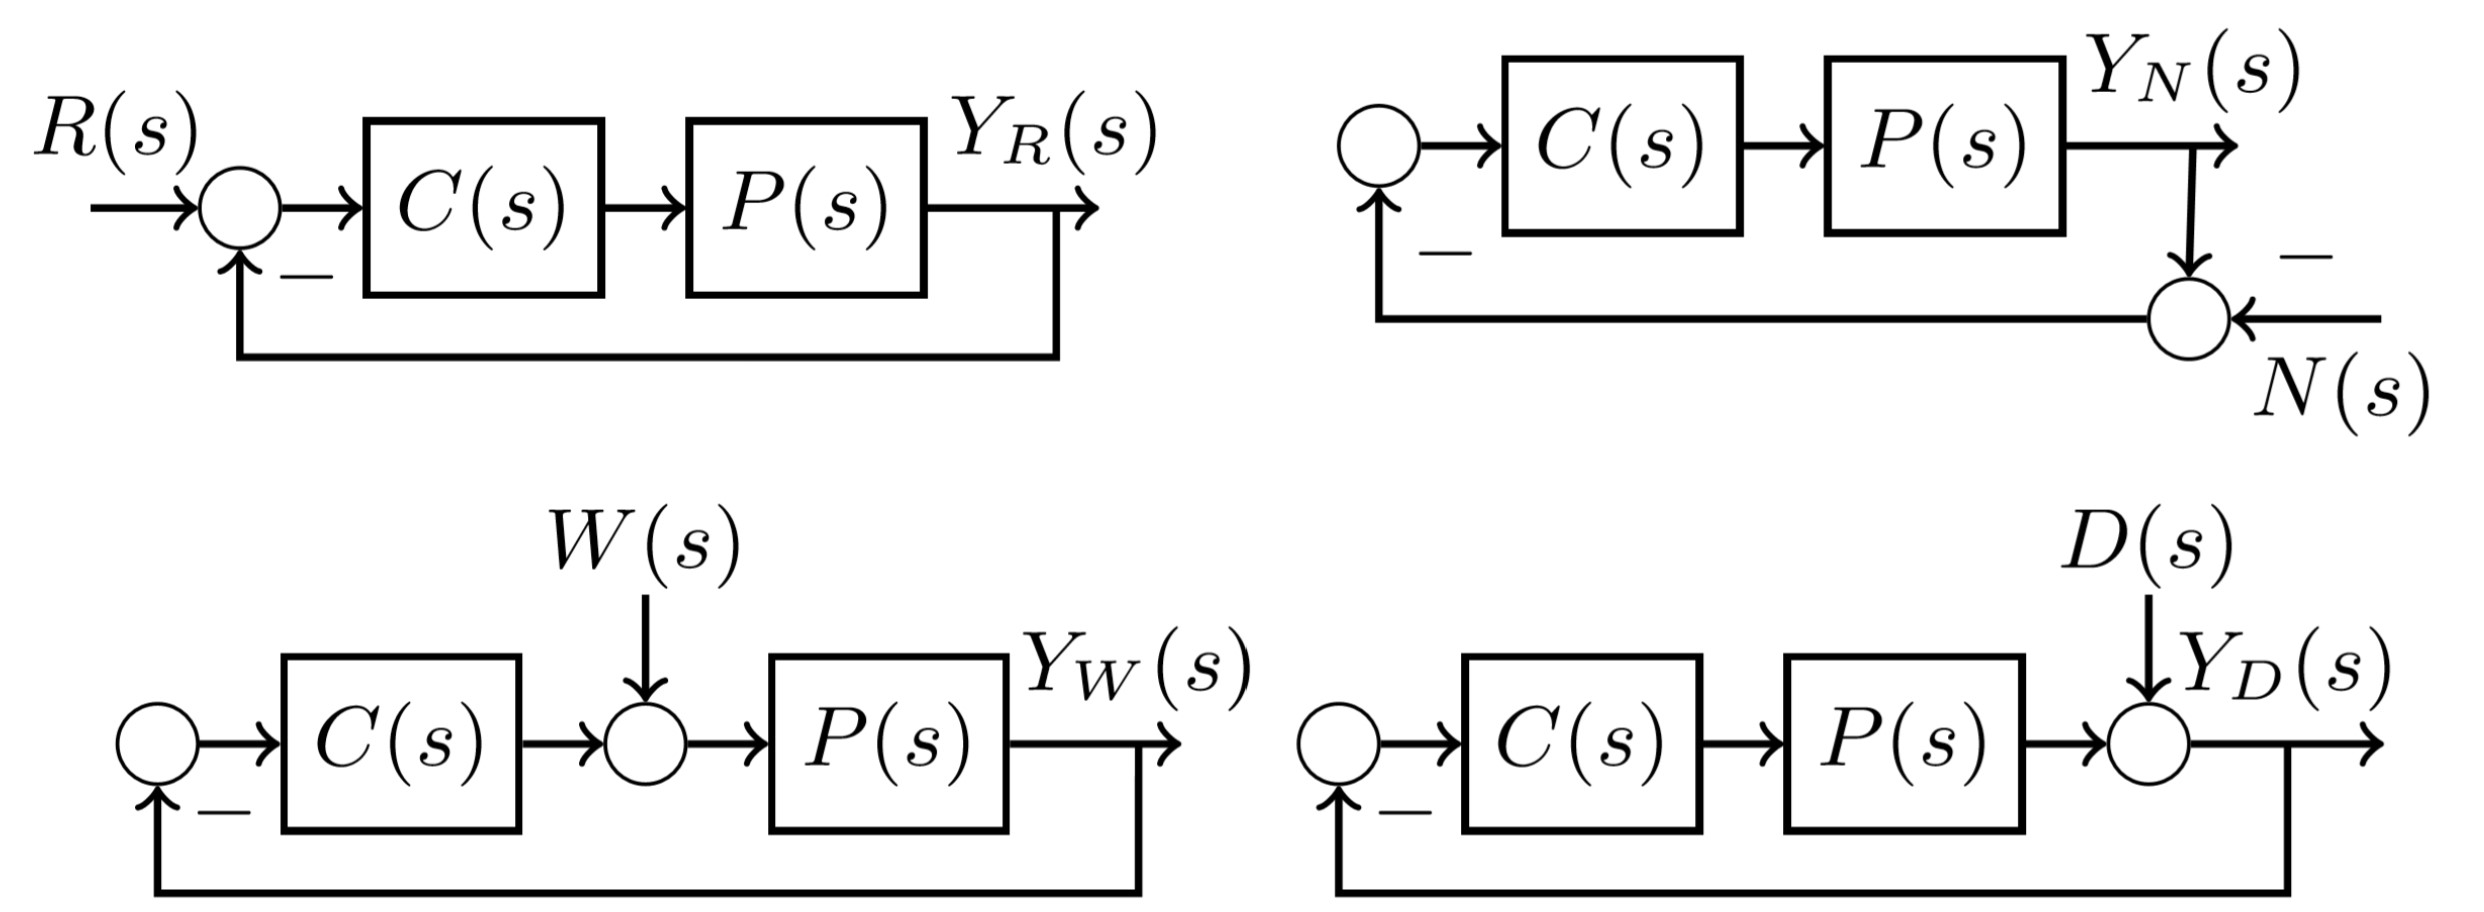
\includegraphics[width = \linewidth]{images/07/Eingangsbeitraege.jpg}
    
    Daraus folgt: 
    \[\begin{matrix}
    Y_R(s) = \frac{P(s)C(s)}{1+P(s)C(s)}\cdot R(s), & Y_N(s) = \frac{P(s)C(s)}{1+P(s)C(s)}\cdot N(s) \\
    &\\
    Y_W(s) = \frac{P(s)}{1+P(s)C(s)}\cdot W(s), &
    Y_D(s) =  \frac{1}{1+P(s)C(S)}\cdot D(s)  

    \end{matrix}\]
    
    Die gesamte Ausgangsgrösse $Y(s)$ lautet somit:
    \[
    Y(s) = Y_R(s) + Y_N(s)+Y_W(s)+ Y_D(s)
    \]
    
    Es Werde folgende Komponenten definiert:
    
    {\renewcommand{\arraystretch}{1.5}
    \begin{tabular}{l|c|c}
    
    \textbf{Kreisverstärkung}    &$L(s)=P(s) C(s)$   & $(e\rightarrow y)$ \\
     \textbf{Sensititvität}  & $S(s) = \frac{1}{1+L(s)}$  & ($d\rightarrow y$, $r\rightarrow e$)   \\ 
     \multirow{2}{10em}{
      \textbf{Komplementäre} \textbf{Sensitivität}} & &\\& $T(s) = \frac{L(s)}{1+L(s)}$ &($r\rightarrow y$, $n\rightarrow y$)
      
        
    \end{tabular}
    }
    Grundsätzlich gilt: \[\textrm{übertragungsfunktion}=\frac{\textrm{Vorwärtspfad}}{1+\textrm{Kreisverstärkung}}\]
    
    \subsection{Stabilität des geschlossenen Regelkreises}
        Für geschlossene Regelkreise muss das Konzept der Stabilität erweitert werden. Ein System ist \textbf{intern stabil}, wenn \textit{alle} Übertragungsfunktionen, welche die Eingänge \textit{w, d, r} im Regelkreis auf die Ausgänge \textit{u, y, e} abbilden, asymptotisch stabil sind ($\textrm{Re}(\lambda_i)<0,\forall i=1,\dots n)$. Die Beziehungen sind durch diese Matrix gegeben:
        \[\begin{bmatrix}
        U(s)\\Y(s)\\E(s)
        \end{bmatrix}
        =
        \begin{bmatrix}
        S(s)    &   -S(s)\cdot C(s) &   S(s)\cdot C(s)\\
        S(s)\cdot P(s)  &   S(s)    &   T(s)\\
        -S(s)\cdot P(s) &   -S(s)   &   S(s)
        \end{bmatrix}
        \cdot
        \begin{bmatrix}
        W(s)\\D(s)\\R(s)
        \end{bmatrix}
        \]
        $\Rightarrow S(s),T(s),S(s)\cdot C(s), S(s)\cdot P(s)$ dürfen nur asymptotisch stabile Pole haben.
        
        Falls $P(s)$ und $C(s)$ nur asymptotisch stabile Pole haben, genügt es also, die asymptotische Stabilität von $S(s)$ oder $T(s)$ zu überprüfen um interne Stabilität zu garantieren.
        
        Wenn wir nur an $r\rightarrow y$ interessiert sind darf das \textbf{charakteristische Polynom} $1+L(s)=0$ nur NST mit $Re(\zeta)<0$ haben. (Falls $C(s)$ oder $P(s)$ instabile Pole haben muss interne Stabilität separat noch überprüft werden.)
        %\TODO{Interne Stabilität muss nur geprüft werden, wenn P oder C instabile Pole hat, sonst genügt es, die Nullstellen von 1+L(s) zu überprüfen. von RT.. stimmt das? chonnt mer vonere üebigsstond bekannt vor.. mösst aber nomol nacheluege}


    \subsection{Nyquist Theorem}
            Durch das Nyquist Theorem kann die asymptotische Stabilität eines geschlossenen Regelkreissystems $T(s)=\frac{L(s)}{1+L(s)}$ durch Analyse seiner Kreisverstärkung $L(s)$ (offener Regelkreis) bestimmt werden. Dabei wird angenommen, dass keine Modellunsicherheit $W_2(s)$ vorhanden ist.
% \vfill\null\columnbreak            
        \subsubsection{Nominelles Stabilitätskriterium von Nyquist}
            Der geschlossene Regelkreis mit Übertragungsfunktion $T(s)$ ist asymptotisch stabil, falls für $L(s)$ gilt:
            \[n_c\overset{!}{=}\frac{n_0}{2}+n_+\]
            \begin{tabular}{l l}
                $n_c$:  & Anzahl Umrundungen um den kritischen Punkt (-1,0)  \\
                        & Positiv falls Umrundung gegen Uhrzeigersinn.\\
                $n_0$:  & Anzahl Pole von $L(s)$ mit Realteil = 0\\
                $n_+$:  & Anzahl Pole von $L(s)$ mit Realteil $>$ 0
            \end{tabular}
            \textbf{Wichtig:} Stabilität nach Nyquist gilt nur, falls \textbf{keine Kürzung von instabilen Polen mit nicht minimalphasigen NST auftreten} in $L(s)=C(s)\cdot P(s)$.
            Andernfalls kann nicht von $L(s)$ auf die interne Stabilität des geschlossenen Regelkreises geschlossen werden.
        \subsubsection{Vorgehen zu Auswertung des Stabilitätskriteriums}
            \begin{enumerate}
                \item Betrachte das Nyquist-Diagramm von $L(j\omega)$ in der komplexen Ebene mit $\omega\in 0,\infty)$.
                \item Spiegle das Diagramm um die reelle Achse. Die gespiegelte Kurve entspricht dem Bereich $\omega \ in (-\infty,0]$. die kombinierte Kurven entspricht also $L(j\omega)$, $\omega \in (-\infty,\infty)$
                \item Zähle $n_c$ die Anzahl Umrundungen von $L(j\omega)$ um den Punkt $(-1+j0)$ wenn $\omega$ von $-\infty$ bis $\infty$ variiert wird. Ein Umlauf in $\circlearrowleft$ wird positiv gezählt, und in $\circlearrowright$ negativ.
            \end{enumerate}
            
    \subsection{Verstärkung und Phasenreserve}
        \begin{wrapfigure}[10]{r}{0.4\linewidth}
        \vspace{-4mm}
            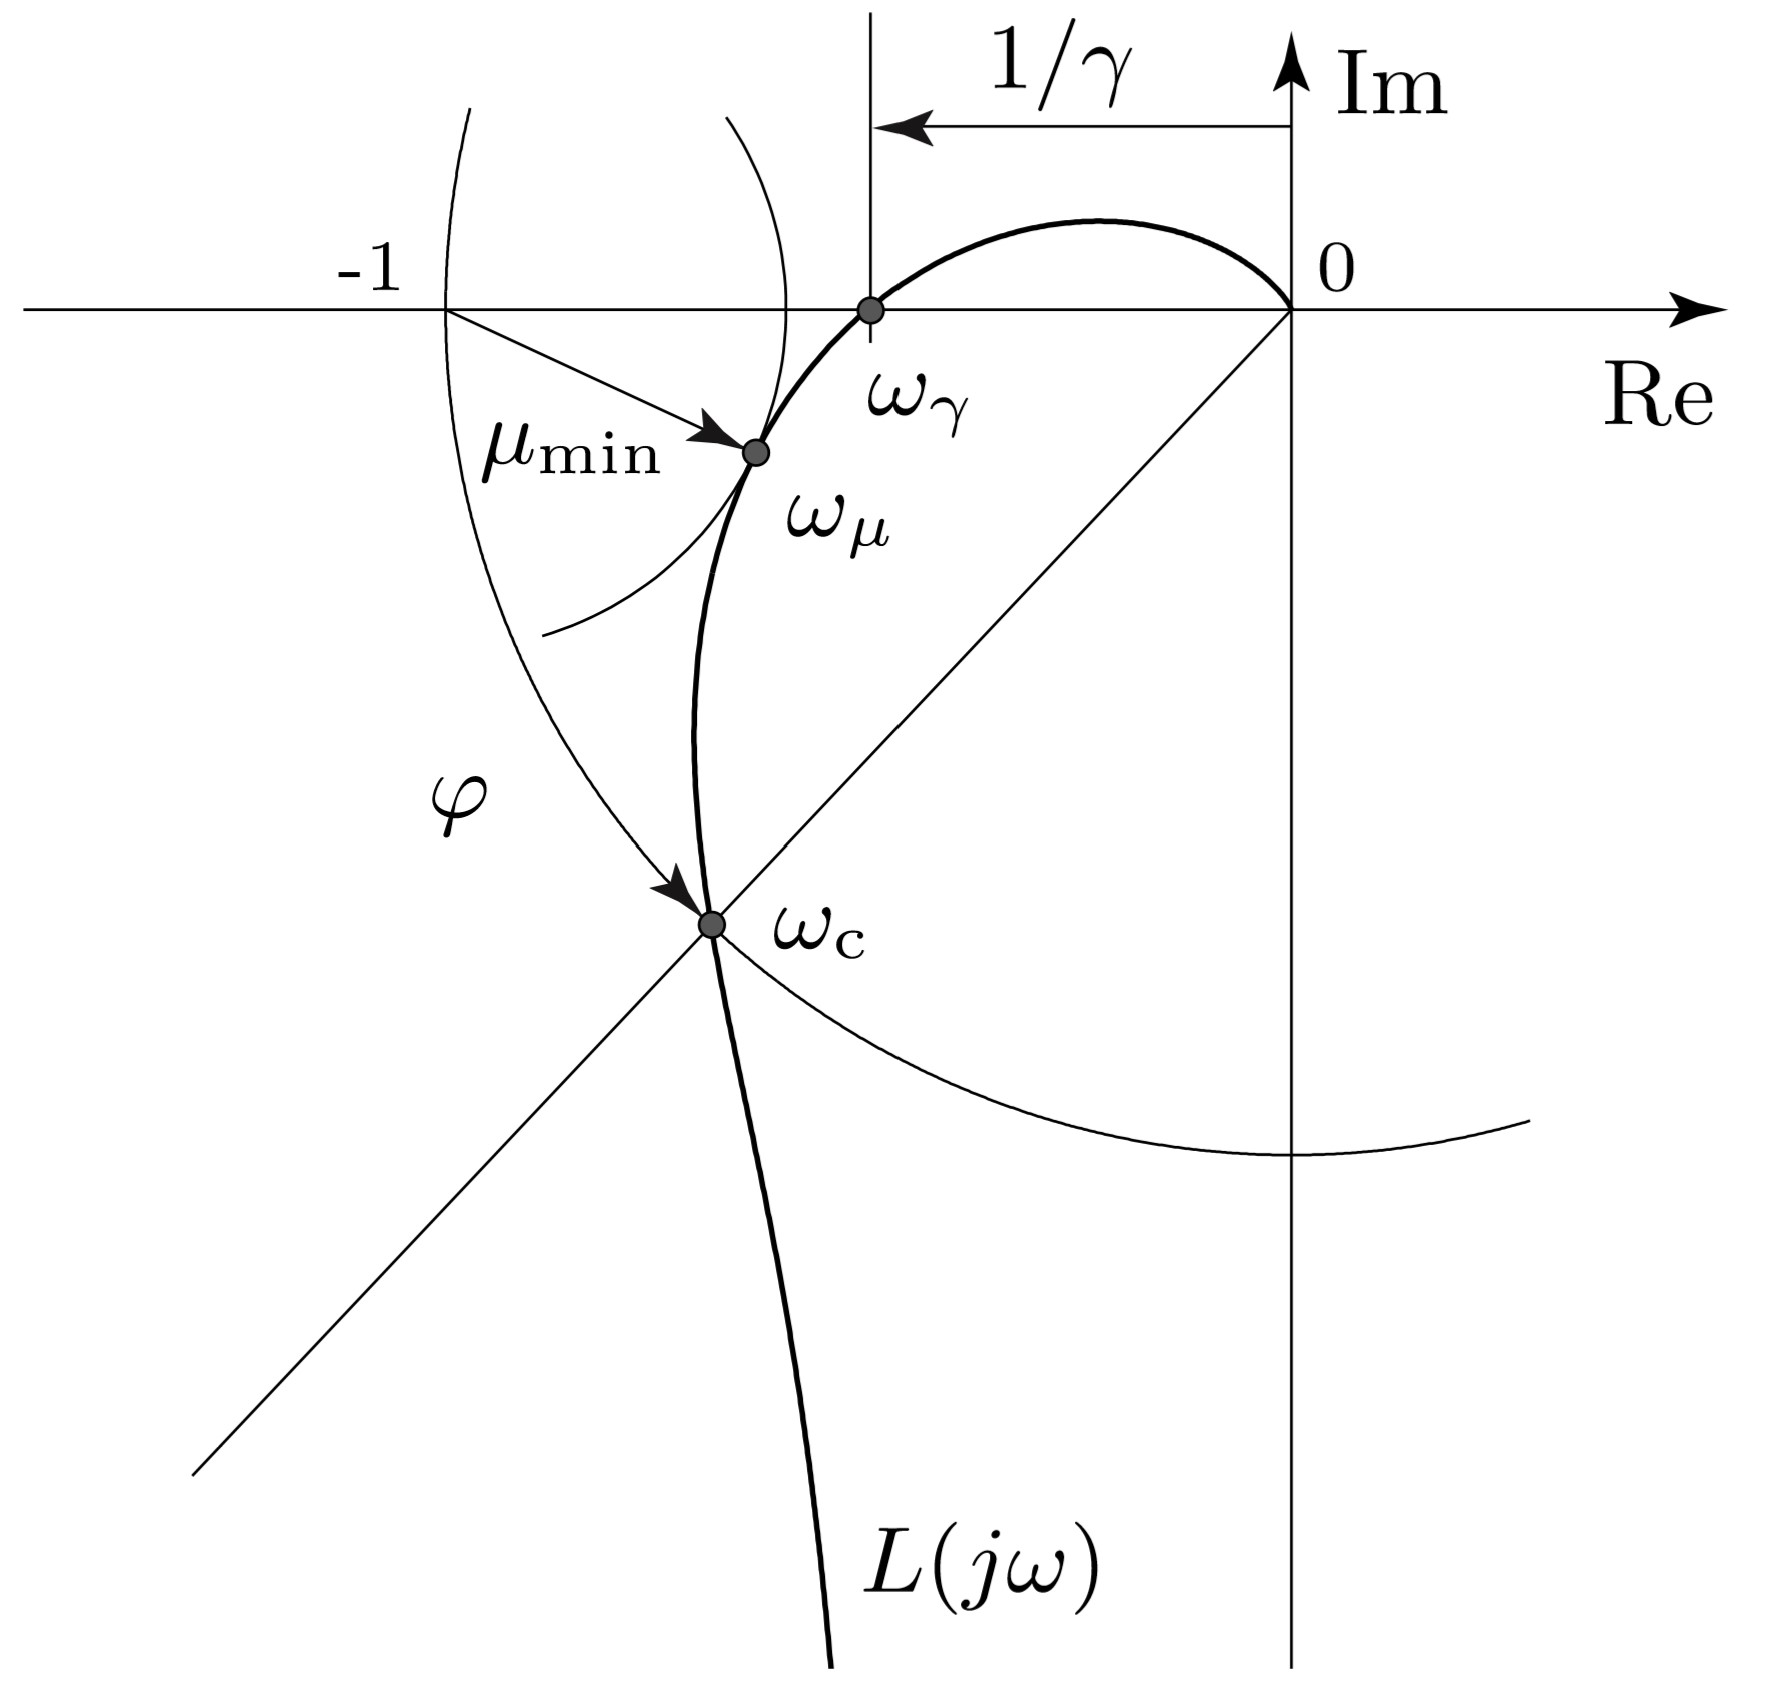
\includegraphics[width=\linewidth]{images/07/Robustheit.jpg}
        \end{wrapfigure}
        Falls $L(s)$ eines Systems das nominelle Stabilitätskriterium \textbf{nicht erfüllt}, hat das resultierende $T(s)=\frac{L(s)}{1+L(s)}$ instabile Pole. 
        
        Falls $L(s)$ eines Systems das nominale Stabilitätskriterium \textbf{erfüllt} kann mittels Verstärkungs- und Phasenreserve eine Aussage bezüglich der Stabilität (Robustheit) gemacht werden. 
\vfill\null\columnbreak
        Es werden drei Robustheitsmasse eingeführt:
        
        \begin{tabular}{|l|c|c|}
        \hline
        &&\\
        $\gamma$    & Verstärkungsreserve & \multirow{2}{14em}{Verstärkungsreserve zu $(-1+0j)$ bei $\angle L(j\omega) = -\pi$}\\
        &&\\
        \hline
        &&\\
        $\varphi$    & Phasenreserve& \multirow{2}{14em}{Phasenabstand zu $-\pi$ bei der Durchtrittsfrequenz $\omega_c$} \\
        &&\\
        \hline
        &&\\
        $\mu$ & kritische Abstand &\multirow{2}{14em}{Kleinste Distanz zwischen $(-1+0j)$ und $L(j\omega)$ } \\
        &&\\
        \hline
        \end{tabular}
        Phasenreserve bei instabilen Systemen nicht well defined
        \[\mu = min_{\mu} |1+L(j\omega)| = \frac{1}{max_\omega|S(j\omega)|}\]
        \subsubsection{Vorgehen um Phasenreserve herauszufinden}
        Um die Phasenreserve berechnen zu können, muss man die Phasen des offenen Regelkreises bei der Durchtrittsfrequenz berechnen.
        \begin{enumerate}
            \item Die Durchtrittsfrequenz durch Lösen der Gleichung $|C(j\omega_c)\cdot P(j\omega_c)| = 1$ 
            \item Nun wird die Phase bei der Durchtrittsfrequenz $\omega_c$ ausgerechnet. $\angle(L(j\omega_c)$
            \item Um die Phasenreserve auszurechnen wird $-\pi$ mit der soeben erhaltenen Phase bei der Durchtrittsfrequenz     subtrahiert
        \end{enumerate}
        
        \subsubsection{Bsp}
            Das nominelle System $L(s)$ hat Phasenfehler $\alpha$ oder Verstärkungsfehler $k$ gegenüber dem wahren System: 
            \[L_{t,\alpha}(s) = e^{-\alpha \cdot s / \omega_c}\cdot L(s), \hspace{4mm} L_{t,k}(s) = k\cdot L(s) \]
            $L_{t,\alpha}$ ist stabil für $\alpha <  \varphi$ und $L_{t,k}$ für $k<\gamma$. Falls beide Fehler gleichzeitig vorhanden sind, sind $\gamma$ und $\varphi$ keine guten Robustheitsmasse, Sie messen beide nur eindimensional.
                
        \subsection{Auslesen der Reserven bei Bode-Diagrammen}
            \begin{center}
                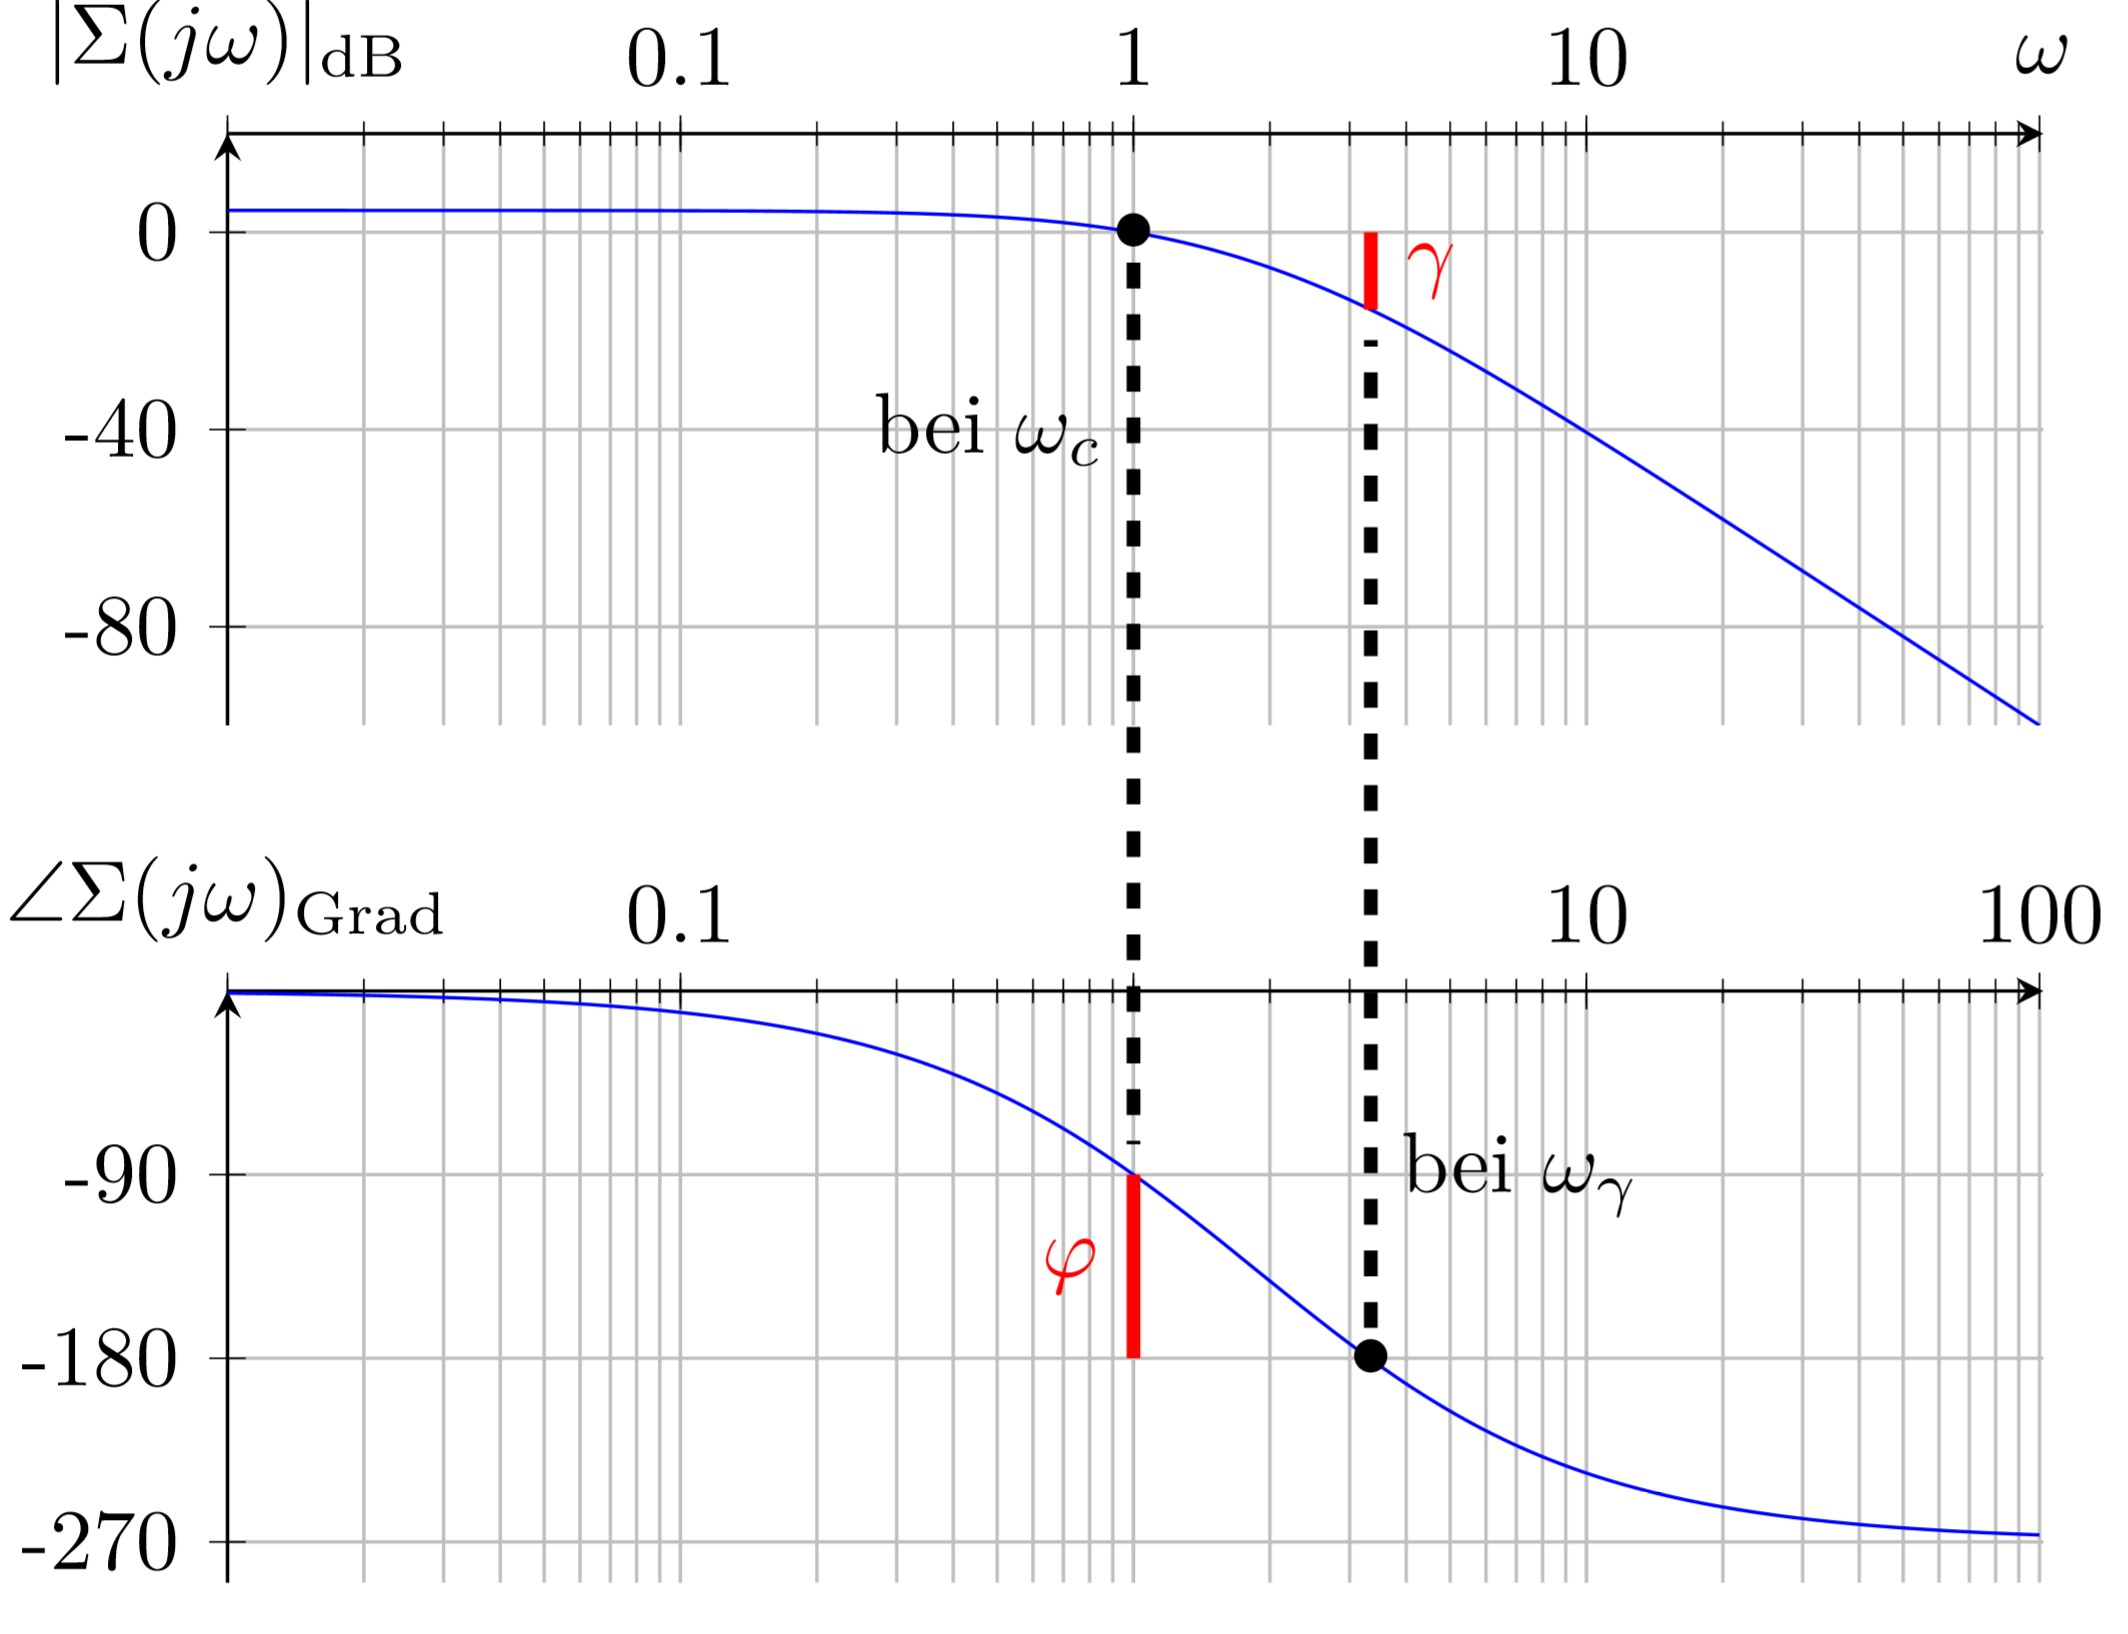
\includegraphics[width=0.7\linewidth]{images/07/reserven_im_bode.jpg}
            \end{center}
    \subsection{Robustes Nyquist Theorem}
        Ein wahres Modell der linearen und zeitinvarianten Regelstrecke $P_t(s)$ existiert, ist aber wegen Modellierungsunsicherheit nicht bekannt. Stattdessen wurde ein Nominalmodell der Regelstrecke $P(s)$ und eine zugehörige multiplikative Unsicherheitübertragungsfunktion $W_2(s)$ gefunden. Der Regler $ C(s)$ ist exakt bekannt. die wahre Kreisverstärkung des Systems $L_t(s) = P_t(s) \cdot C(s)$ ist Teil der Menge $\mathcal{S}_\mathcal{L}$:
        \[\mathcal{S}_\mathcal{L} = \{P(s)\cdot C(s) \cdot (1+\Delta \cdot W_2(s))\}\]
        \[\textrm{mit} |\Delta| \leq 1, \angle\Delta \in [-\pi,\pi]\]
        
        Es wird angenommen, dass $L(s)$ und $L_t(s)$ dieselbe Anzahl instabile $(n+)$ und stabile $(n_0)$ Pole haben.
        
        \subsubsection{Robustes Stabilitätskriterium von Nyquist}
            Das robuste Stabilitätskriterium von Nyquist wird aus dem nominalen Nyquist-Stabilitätskriterium abgeleitet: Falls nämlich das nominale Nyquist-Stabilitätskriterium für jedes $ L_t(j\omega)\in\mathcal{S}_\mathcal{L} $ in Gl.(3) erfüllt ist, dann ist der Regelkreis garantiert asymptotisch stabil.
          
            Umsetzung des robusten Stabilitätskriteriums: Durch betrachten der grössen Modellunsicherheit, d.h. mit $|\Delta|=1$ und für alle möglichen Richtungen (Phasen) von $\Delta$ beschränken wir unsere Überlegung auf den schlimmst möglichen Fall, d.h. 
            \[L_t(s) = L(s) + L(s)\cdot W_2(s)\]
            $\Rightarrow$ Kreise die durch $(0,0)$ gehen.
 \vfill\null\columnbreak          
            Um zusätzliche Umkreisungen des Punktes (-1+0j) garantiert zu verhindern, darf der Unsicherheitsradius \textcolor{red}{$|L(j\omega)\cdot W_2(j\omega)|$} nie grösser als \textcolor{blue}{$|1+L(j\omega)|$} werden. Daraus folgt das robuste Stabilitätskriterium nach Nyquist:
            
            \[|L(j\omega)\cdot W_2(j\omega)| < |1+L(j\omega)|,\forall\omega\in[0,\infty)\]
            
            \begin{center}
                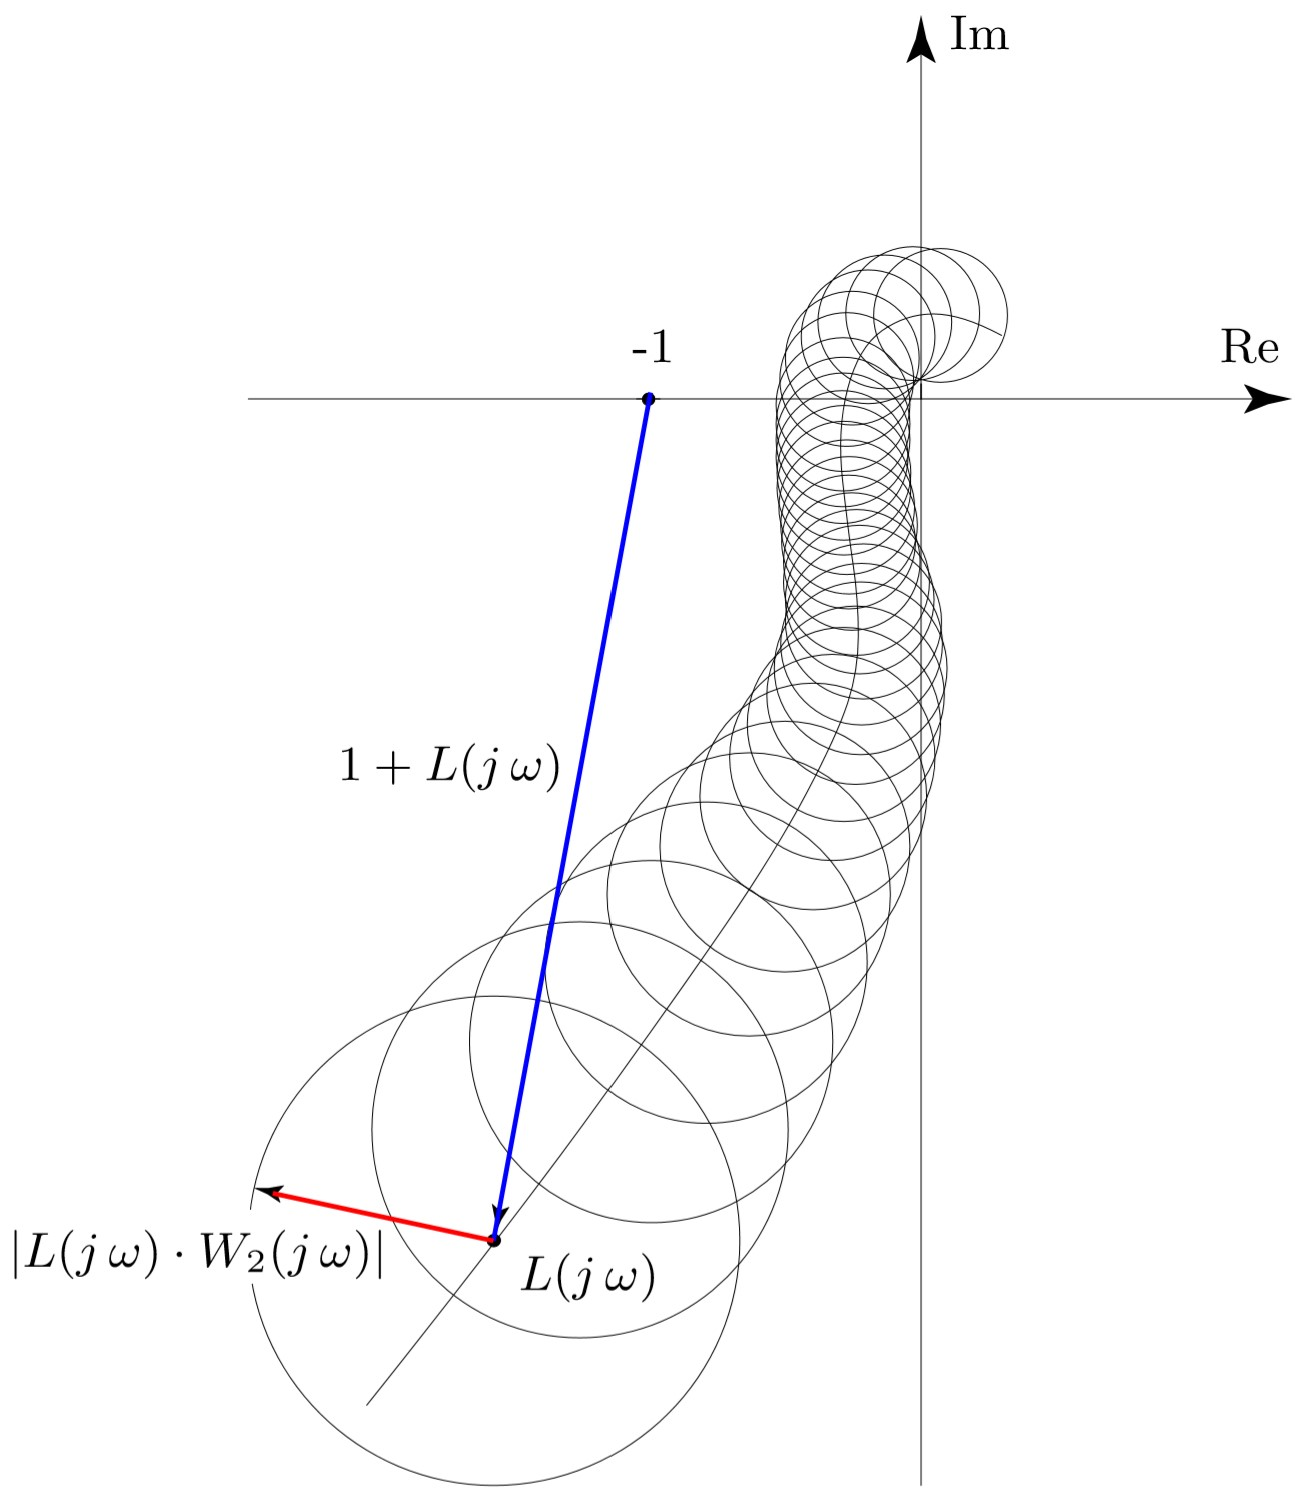
\includegraphics[width = 0.6\linewidth]{images/07/Robustes_nyq_Stabkrit.jpg}
            \end{center}
\vfill\null\columnbreak
\section{Design von Regelungssystemen}
    \subsection{Frequenzbedingung des geschlossenen Regelkreises}
        \subsubsection{Frequenzeigenschaften von Störungen und Rauschen}
            Die Übertragungsfunktionen des geschlossenen Regelkreises $S(s)$ und $T(s)$ sind intrinsisch gekoppelt:
            \[T(s) + S(s) = \frac{L(s)}{1+L(s)}+\frac{1}{1+L(s)}=1,\forall s\in\mathbb{C}\]
            Dies setzt voraus, dass bei gegebener Frequenz $\overset{*}{\omega}$ entweder $|T(j\overset{*}{\omega}|$ oder $|S(j\overset{*}{\omega})|$ viel kleiner als 1 sein kann.
            \textbf{Störungen} werden mit $S(s)$ auf den Ausgang übertragen und \textbf{Rauschen} mit $T(s)$.
            Die generelle Aufgabe eines Reglers ist die gleichzeitige Unterdrückung von Rauschen und Störungen. Dies ist jedoch nur möglich wenn die Signale in unterschiedlichen Frequenzbändern auftreten. Dabei tritt Rauschen in der Regel bei hohen Frequenzen $(\omega>\omega_n)$ auf und Störungen in der Regel bei tiefen Frequenzen $(\omega<\omega_d)$. Daraus ergibt sich folgende Erkenntnis:
        
            \textbf{Niedrige Frequenzen} $\boldsymbol{\omega<\omega_d}$
            \[|S(j\omega)| = \bigg|\frac{1}{1+L(j\omega)}\bigg|  \overset{!}{<<} 1 \Rightarrow 
            |L(j\omega)| >> 1 \]
            \textbf{Hohe Frequenzen} $\boldsymbol{\omega > \omega_n}$
            \[|T(j\omega)| = \bigg|\frac{L(j\omega)}{1+L(j\omega)}\bigg|  \overset{!}{<<} 1 \Rightarrow 
            |L(j\omega)| << 1 \]
       
            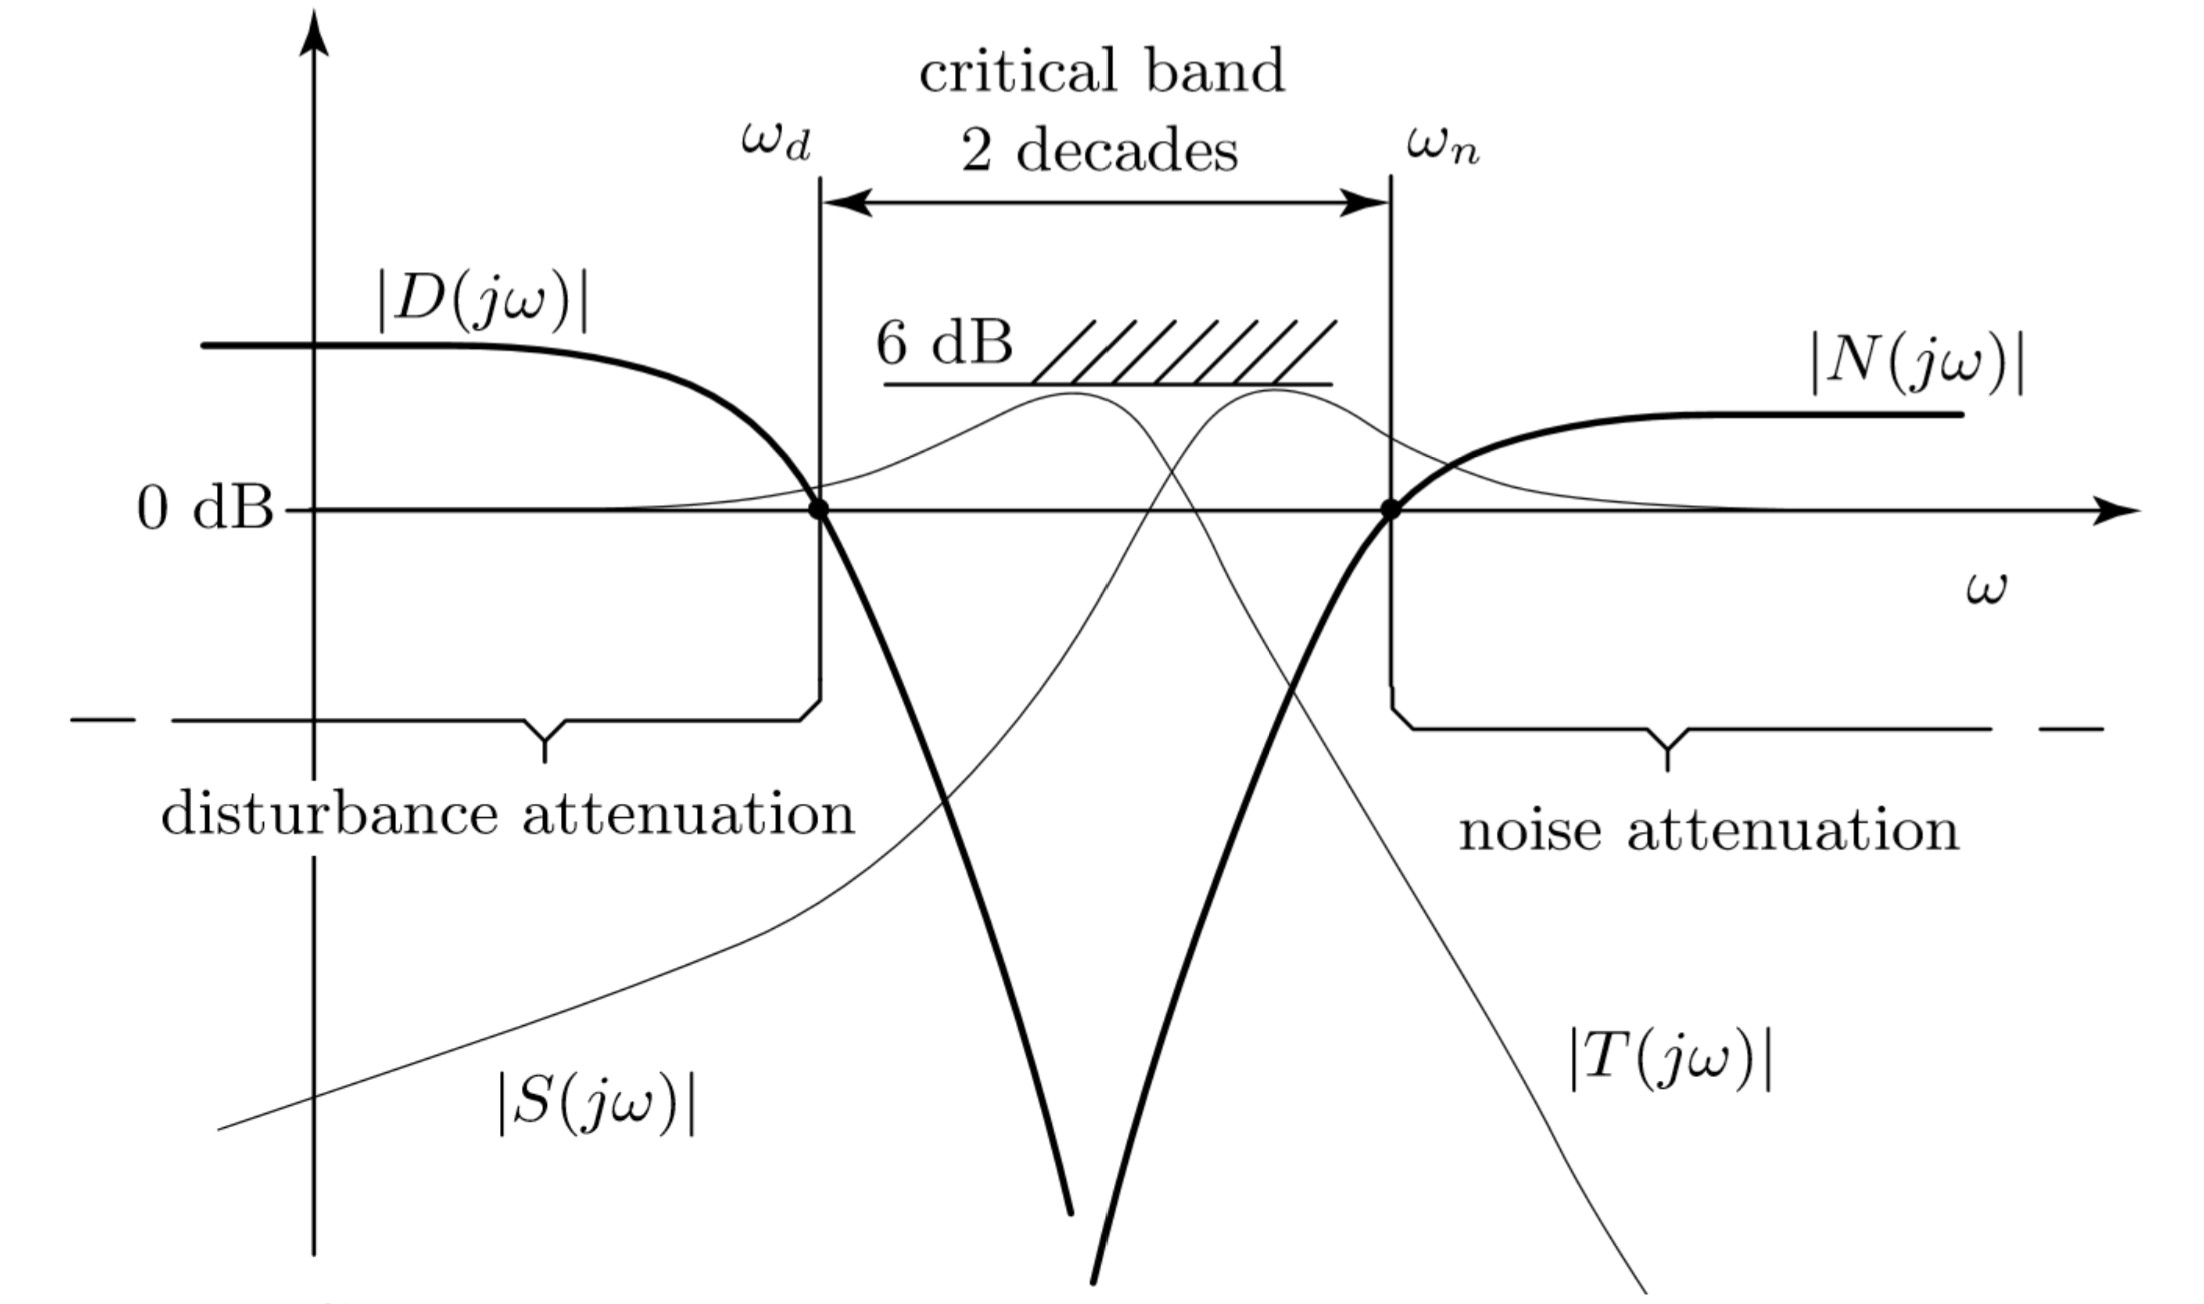
\includegraphics[width = \linewidth]{images/08/Stoerung_und_Rauschen.jpg}
        \subsubsection{Beschränkung der Sensitivität}
            Der Frequenzgang der Sensitivität $S(j\omega)$ kann durch Einstellen des Reglers $C(j\omega)$ lokal beeinflusst werden.
            
            Global betrachtet, über alle $\omega$, muss die Sensitivität für alle stabilen geschlossenen Regelkreise (d.h. Stabilität durch das Nyquist Theorem bestimmt) folgende Gleichung erfüllen:
            \[
            \int_0^\infty ln|S(j\omega)|d\omega = \pi \cdot \sum^{n_+}_{i=1} \pi^+_i
            \]
            
            wobei $n^+$ die Anzahl der instabilen Pole $\pi^+$ der Kreisverstärkung $L(s)$ ist. Diese Gleichung impliziert dass eine Verringerung von $|S(j\omega)|$ in einem Frequenzband durch eine Erhöhung in einem anderen Frequenzband kompensiert wird. Falls die Kreisverstärkung $L(s)$ keine instabilen Pole ($n_+=0$) vereinfacht sich die Gleichung zu:
            \[\int_0^\infty ln|S(j\omega)|d\omega = 0\]
    \subsection{Beschränkung der Durchtrittsfrequenz}
    
        $\omega_c$ ist die \textbf{Durchtrittsfrequenz}, und entspricht der Frequenz bei der das Bode-Diagramm von $L(j\omega)$ die 0dB-Linie schneidet\\
        $\omega_b$ ist die \textbf{Bandbreite} des geschlossenen Regelkreises. Die Bandbreite ist ein Mass für die höchste Frequenz des Eingangssignals, die der geschlossene Regelkreis verfolgen kann.
        
        Beim \textbf{geschlossenen Regelkreis:} $\omega_b:=|T(j\omega_b)|=-3dB\approx 0.7$\\
        Die Bandbreite entspricht ungefähr der Durchtrittsfrequenz. $\boxed{\omega_b\approx\omega_c}$

        Zusammenfassend kann man folgende Formel für die Beschränkung Anwenden:
        
        \[\boxed{\omega_c = 
        \begin{cases}
        \omega_c > \textrm{max}\{10\cdot\omega_d, 2\cdot\omega_{\pi^+}\}\\
        \omega_c < \textrm{min}\{\frac{1}{10}\cdot\omega_n, \frac{1}{10}\cdot \omega_2, \frac{1}{2}\cdot \omega_\tau, \frac{1}{2}\cdot \omega_{\zeta^+}\}
        \end{cases}
        }
        \]
        
        \subsubsection{Beschränkung durch Modellunsicherheiten $W_2$}
            aus dem robusten Stabilitätskriterium folgt: 
            \[|L(j\omega)\cdot W_2(j_\omega)| < |1+L(j\omega)|, \forall \omega\in[0,\infty)\]
            \[\Rightarrow \bigg|\frac{L(j\omega)}{1+L(j\omega)}\bigg|<\bigg|\frac{1}{W_2(j\omega)}\bigg|\]
            \[\Rightarrow |T(j\omega)|<\big|W_2^{-1}(j\omega)\big|\]
            Da die Unsicherheit $|W_2(j\omega)|$  tendenziell mit der Frequenz zunimmt
            ergibt sich dadurch eine \textbf{obere} Grenze der Bandbreite, und somit eine Beschränkung der Durchtrittsfrequenz von $|L(j\omega)|$.
            
            Man will die Unsicherheit auf jeden Fall vermeiden. Deswegen wählt man als obere Schranke für die Durchtrittsfrequenz eine Dekade kleiner als die Unsicherheitsfrequenz.
            \[\boxed{\omega_c\overset{!}{<}\mathbf{\frac{1}{10}}\cdot\omega_2} \hspace{5mm}|W_2(j\omega_2)|=1\]
        \subsubsection{Beschränkung durch eine Totzeit $\tau$}
            Die Übertragungsfunktion der Kreisverstärkung mit Verzögerung im Regler und der Regelstrecke ist gegeben durch: 
            \[L_\tau(s) = C(s)\cdot P(s)\cdot e^{-(\tau C + \tau P)\cdot s} = C(s) \cdot P(s) \cdot e^{-\tau\cdot s}\]
                
            Die Totzeit induziert eine \textbf{obere} Grenze für die Durchtrittsfrequenz. Um die Totzeitsfrequenz gut zu vermeiden wird als Grenze die halbe Totzeitfrequenz gewählt.
            \[\boxed{\omega_c \overset{!}{<}\mathbf{\frac{1}{2}} \cdot \omega_\tau = \frac{1}{2}\cdot\frac{1}{\tau}}\hspace{5mm} (\textrm{konservativer mit } \mathbf{\frac{1}{5}} \textrm{ als Faktor)}\]
        \subsubsection{ Beschränkung durch nicht-minimalphasige Nullstellen $\omega_{\zeta^+}$}
        Gegeben sei eine Regelstrecke $P(s) = \frac{n(s)}{d(s)}$ mit mindestens einer nicht-minimalphasigen Nullstelle. Um die Wirkung der Nullstellen zu veranschaulichen, wählt man einen konstanten Regler $C(s) = k_p$, $k_p \in \mathbb{R}$.
        \[S(s) = \frac{d(s)}{d(s)+k_p\cdot n(s)}, \hspace{5mm} T(s) = \frac{k_p\cdot n(s)}{d(s)+k_p\cdot n(s)}\] 
        
        Wenn $k_p \rightarrow \infty$ strebt, nähern sich die Pole von $S(s)$ und $T(s)$, gegeben durch $d(s)+k_p \cdot n(s) = 0 $, an die Lösung von $n(s) = 0$. Da $n(s)$ mindestens eine nicht-minimalphasige Nullstele hat, wird das System bei $k_p = k_{p,\textrm{crit}}$ instabil. Dies impliziert, dass die Bandbreite durch eine \textbf{obere} Grenze beschränkt ist.
        \[\boxed{\omega_c \overset{!}{<} \mathbf{\frac{1}{2}} \cdot\omega_{\zeta^+}} \hspace{5mm} (\textrm{konservativer mit } \mathbf{\frac{1}{5}}\textrm{ als Faktor})\]
        
        \subsubsection{Beschränkung durch instabile Pole $\pi^+$}
            \begin{itemize}
                \item \textbf{Instabile Pole $\mathbf{\pi^+}$ ohne Modellierungsunsicherheit}

                Nominelles Stabilitätskriterium von Nyquist prüfen der Regler so auslegen, dass das Kriterium für die Kreisverstärkung $L(S)$ erfüllt ist
                
                Daraus folgt eine \textbf{untere} Schranke für die Durchtrittsfrequenz:
                
                \[\boxed{\omega_c>\mathbf{2}\cdot \omega_{\pi^+}}\hspace{5mm} (\textrm{konservativer mit } \mathbf{5}\textrm{ als Faktor})\]
                
                \item \textbf{Instabile Pole $\mathbf{\pi^+}$ mit Modellierungsunsicherheit}\\
                zusätzlich zum Vorhergehenden Vorgehen müssen wir für instabile Pole mit Modellierungsunsicherheit zusätzlich noch \[|W_2(\pi_i^+)| <1, \forall i\]
            \end{itemize}
            
    \subsection{Statischer Nachlauffehler}
        Einfluss des Fehlers $e(t)$ im eingeschwungenen Zustand. Dazu wird der Regelkreis im Frequenzbereich betrachtet:
        \begin{center}
            \includegraphics[width = 0.8\linewidth]{images/08/Standart_Regelkreis_FB.jpg}
        \end{center}
        $E(s)$ als Funktion der Eingänge beschrieben: 
    
        \begin{align*}
            E(s) &= E_R(S) + E_N(S) + E_D(s) + E_W(S)\\
            &= \mathbf{S(s)\cdot \left[R(s) + N(s) - D(s) - P(s)\cdot W(s)\right]}
        \end{align*}
        
        Falls der Eingang ($R(s),N(s),-D(s)$) ein Step ist, kann man den Fehler aus dem Endwerttheorem berechnen durch:
        \[e^h_\infty=\lim_{s\to 0_+}s\cdot S(s)\cdot\frac{1}{s}=\lim_{s\to 0_+}S(s)=S(0)\]
        
        \textbf{Achtung:} Aufpassen bei $D(s)$ \& $W(s)$! Bei $D(s)$ das - und bei $W(s)$ multiplizieren mit $-P(s)$ nicht vergessen.
        
        \subsubsection{Bsp}
            \[L_1(s) =\frac{1}{s+1}(k=0),\qquad L_2 =\frac{1}{s(s+1)}(k=1)\]
            \[T_1 =\frac{1}{s+2},\qquad T_2 =\frac{1}{s^2+s+1}\]
            Erstes System hat Systemtyp $k=0$ und weist somit einen Fehler in der Sprungantwort auf: $S_1(0)=\frac{1}{2}$.\\
            Der zweite offene Regelkreis $L_2(s)$ hat Systemtyp $k=1$ ($L_2(s)$ strebt für $s\to 0$ linear gegen $\infty$). Daraus folgt, dass das zweite System fehlerfrei zum Sprung konvergiert.
            \begin{center}
                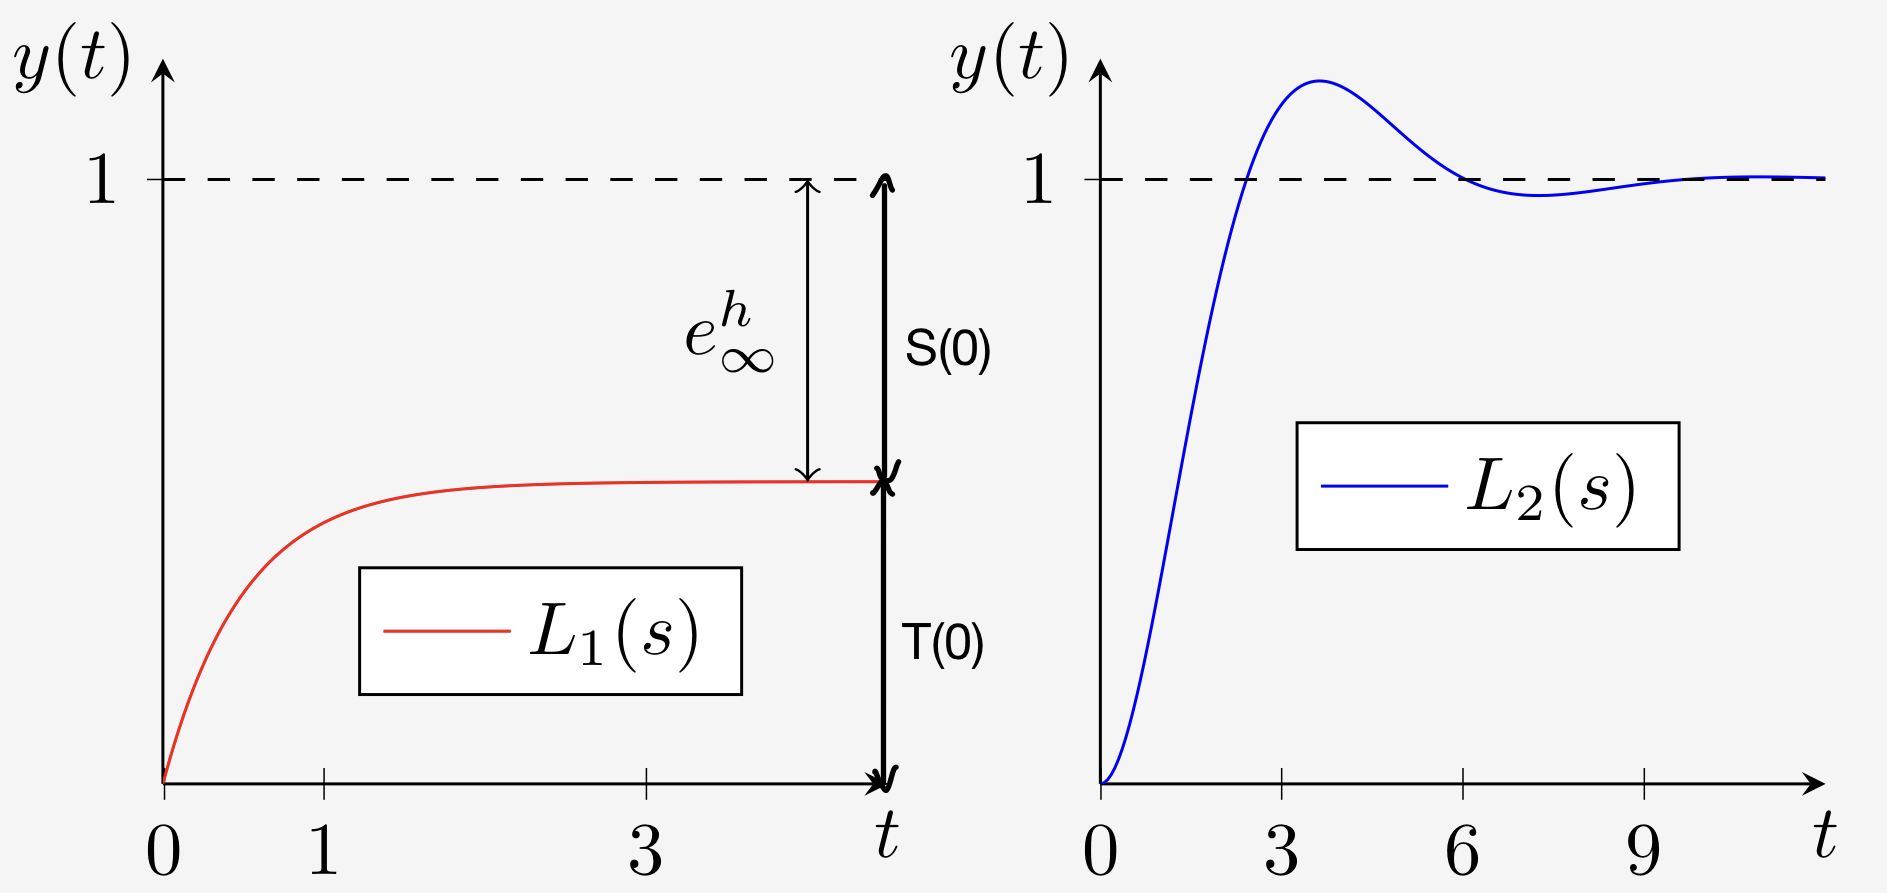
\includegraphics[width=0.8\linewidth]{08/nachlauffehler.jpeg}
            \end{center}

            %$L_1(s)=\frac{1}{s+1}(k=0),\quad L_2=\frac{1}{s(s+1)}(k=1),$
        % man betrachtet Referenzen und Störungen die als Sprünge $h(t)$ auf den Fehler abgebildet werden:
    
        % \[h(t) = 1, \hspace{2mm} t>0 \hspace{3mm} \rightarrow \hspace{3mm} H(s) = \frac{1}{s}\]
    
        % Mit dem Endwerttheorem kann man den Fehler auf eine Sprungantwort nach langer Zeit berechnen: 
        % \TODO{unklar}
    \subsection{Spezifikationen basierend auf   Systeme 2. Ordnung}
        Es wird angenommen, dass der geschlossene Regelkreis $T(S)$ einem System zweiter Ordnung entspricht:
        \[T(s) = \frac{\omega_0^2}{s^2+2\cdot\delta\cdot\omega_0\cdot s+\omega_0^2}\] 
        Dieser Regelkreis $T(s)$ soll Spezifikationen in der Anstiegszeit \textcolor{blue}{$t_{90}$} und im relativen Überschwingen \textcolor{red}{$\hat{\epsilon}$} erfüllen.
        \begin{center}
            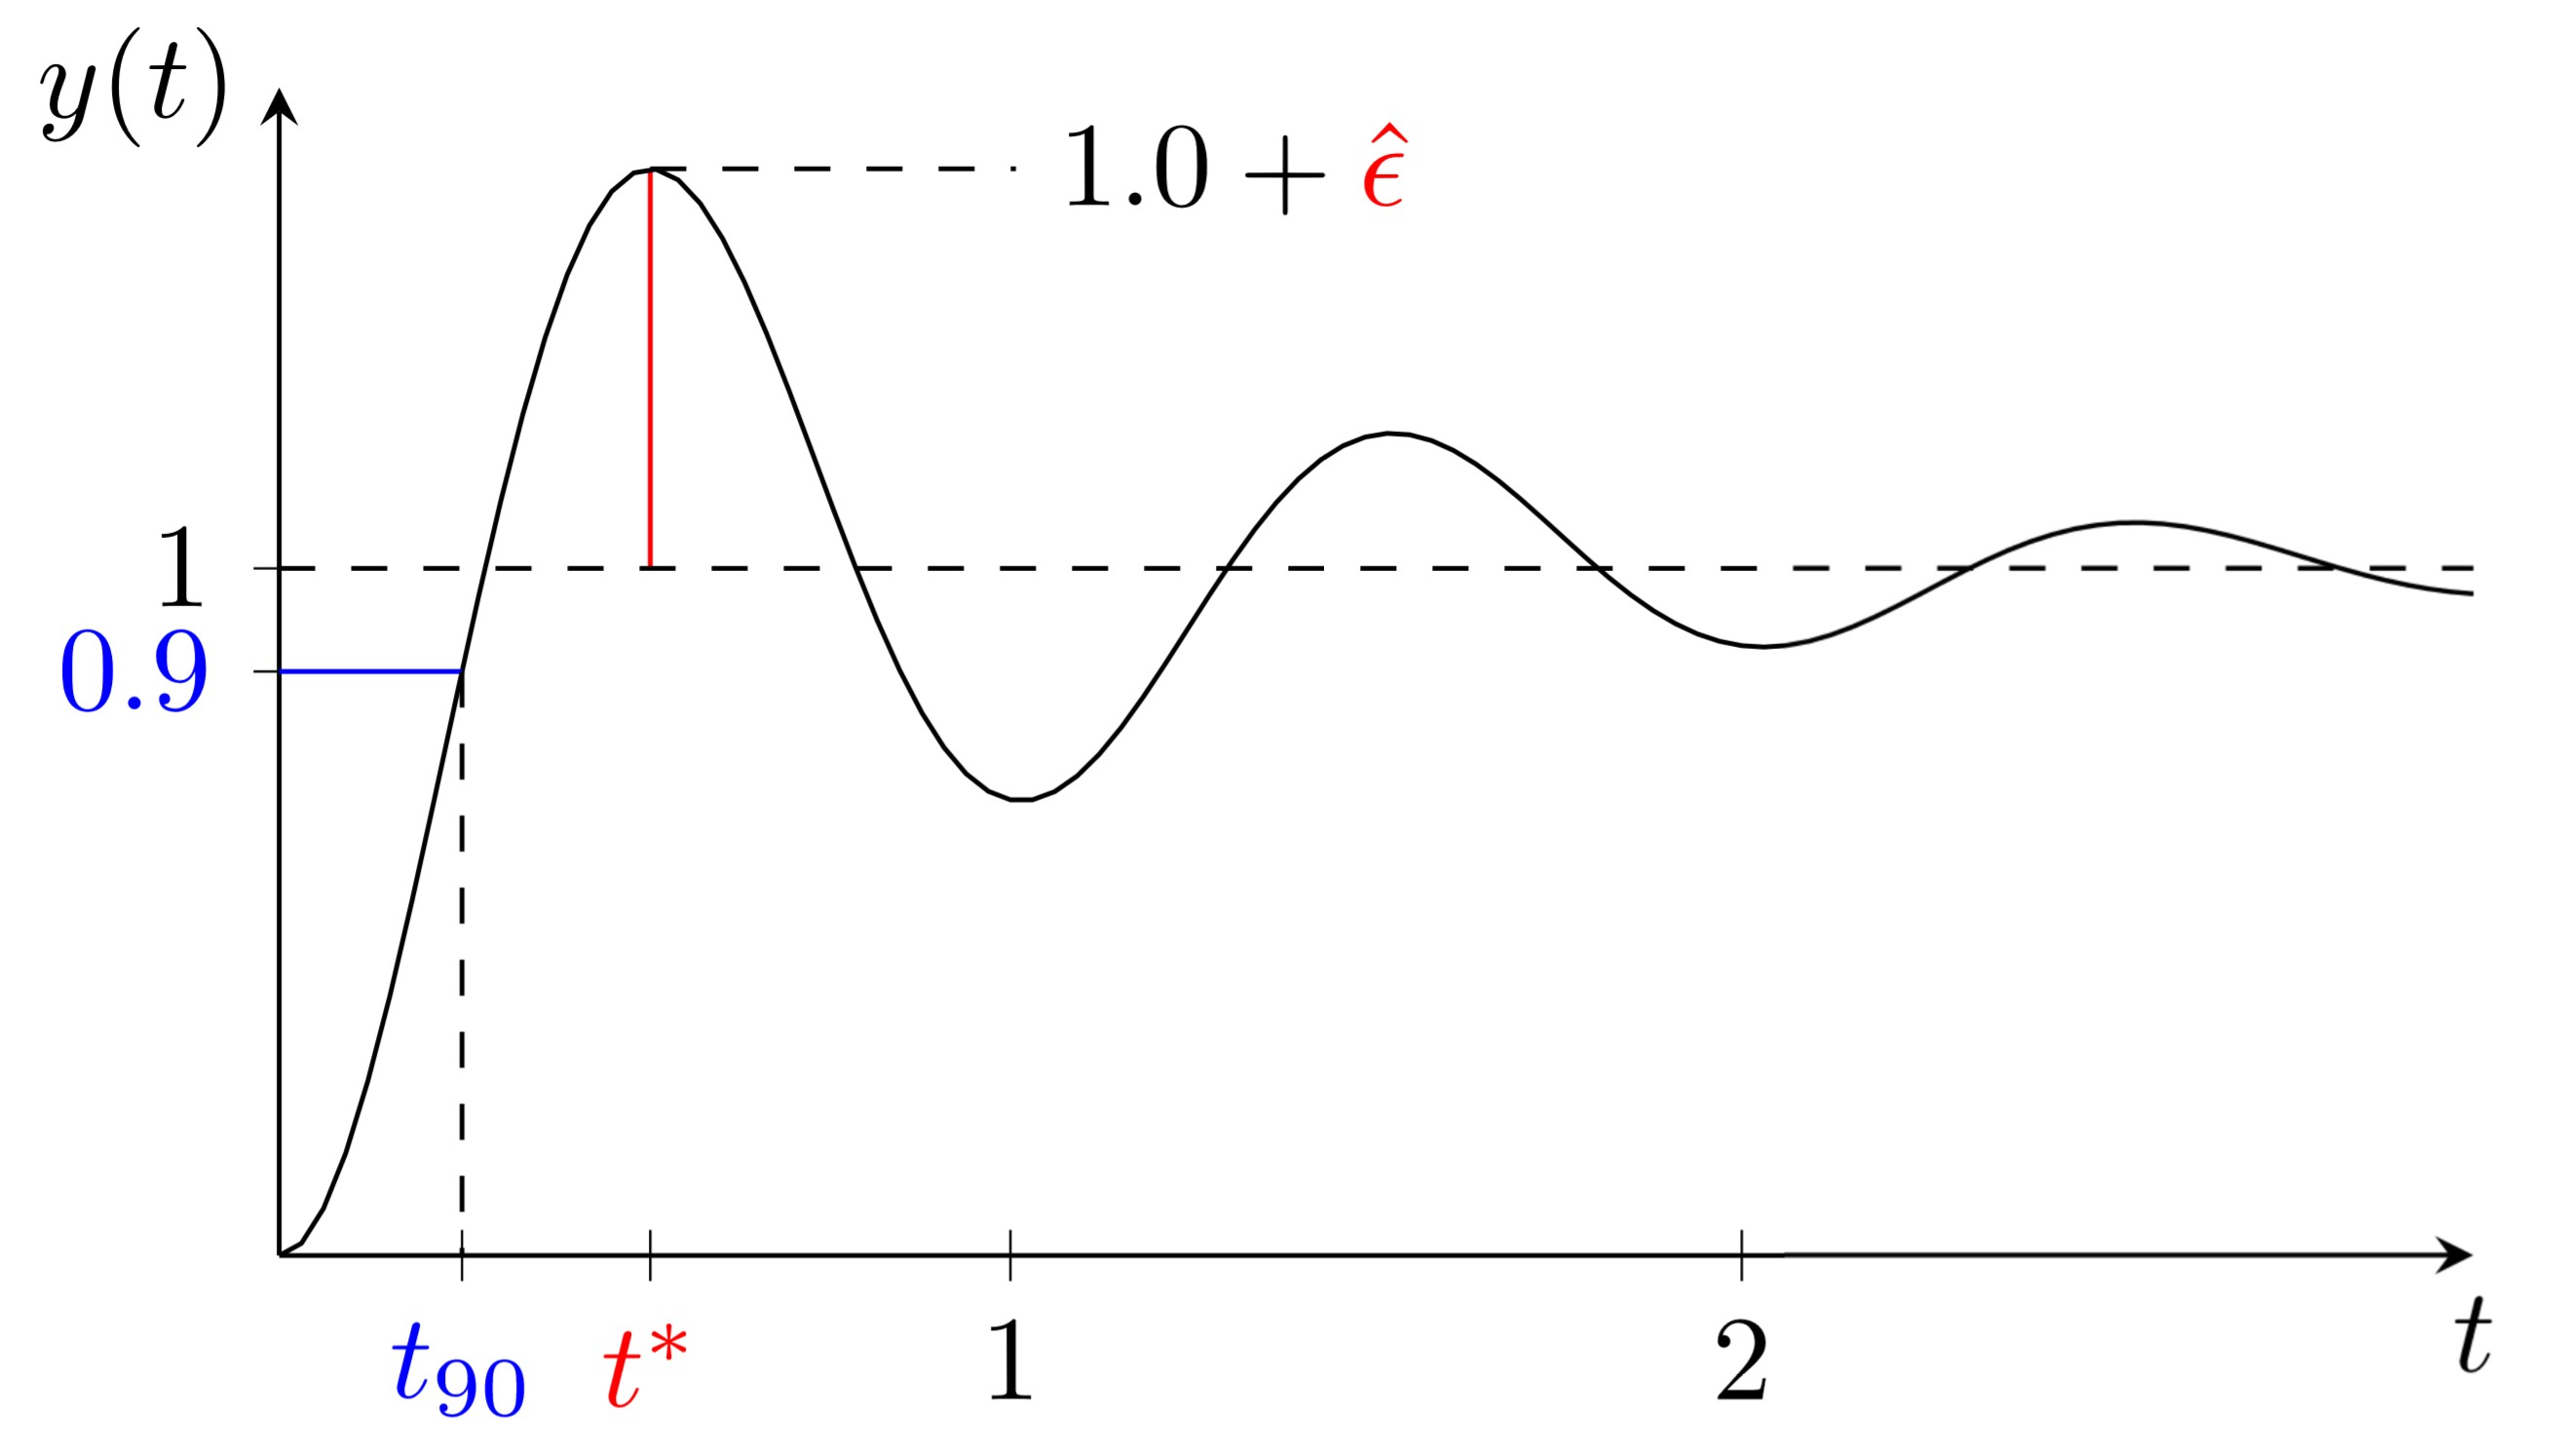
\includegraphics[width = 0.8\linewidth]{images/08/t90_epsilon.jpg}
        \end{center}
    
        gewünschte $\hat{\epsilon}$ und $t_{90}$ können durch auswählen der typischen Parametern eines System 2- Ordnung erreicht werden.
        \[\delta = \frac{-ln(\hat{\epsilon})}{\sqrt{\pi^2+ln^2(\hat{\epsilon})}}, \hspace{3mm} \omega_0 = (0.14 +0.4\cdot\delta)\cdot\frac{2\cdot\pi}{t_{90}} \]
        Nun werden die Spezifikationen an $T(s)$ in Anforderungen an die Kreisverstärkung $L(s)$ umgewandelt, unter Anwendung von $T(s) = \frac{L(s)}{1+L(s)}$.
    
        Die Anforderungen des geschlossenen Regelkreises können in Anforderungen an die Durchtrittsfrequenz $\omega_c$und die Phasenreserve $\varphi$ der Kreisverstärkung $L(s)$ umformuliert werden:
    
        \begin{align*}
            \omega_c &= \omega_0\cdot \sqrt{\sqrt{4\cdot\delta(\hat{\epsilon})^4+1}-2\cdot\delta(\hat{\epsilon})^2}\\
            \varphi &= \frac{\pi}{2}-\arctan\Bigg(\frac{ 
            \sqrt{\sqrt{4\cdot\delta(\hat{\epsilon})^4+1}-2\cdot\delta(\hat{\epsilon})^2}}{2\cdot\delta(\hat{\epsilon})}\Bigg)
        \end{align*}
    
        diese Gleichungen können für $\boxed{0.45<\delta<1}$ mit den folgenden vereinfachten Zusammenhängen angenähert werden:
        \begin{center}
            \begin{tabular}{|l c l|}
                \hline
                &&\\
                $\omega_c$   &  $\approx$ &       $\frac{1.7}{t_{90}}$\\
                &&\\
                $\varphi$   & $\approx$ &         $71^\circ-117^\circ\cdot\hat{\epsilon}    $\\
                &&\\
                \hline
            \end{tabular}
        \end{center}
        (Systeme mit Dämpfungen $\delta$ ausserhalb der Menge $(0.45,1)$ sind in der Praxis nicht relevant, weil sie entweder sehr stark überschwingen oder extrem langsam sind.)
    \subsection{Frequenzbereich - Spezifikationen}
        Die Störung $D(s)$ und das Rauschen $N(s)$ werden durch die Sensitivität $S(s)$ und durch die komplementäre Sensitivität $T(s)$ auf den Ausgang abgebildet:
        \[Y(j\omega) = S(j\omega)\cdot D(j\omega)+T(j\omega)\cdot N(j\omega)\]
        
        Um die Auswirkung von Störungen und Rauschen um die Durchtrittsfrequenz $\omega_c$ zu minimieren, beschränkt man den Maximalwert von $S(s)$ und $T(s)$.
        
        \[
        \|S\|_\infty<S_{max}, \hspace{3mm} \|T\|_\infty < T_{max}, \hspace{3mm} S_{max},T_{max} > 1,
        \]
        wobei per Definition $\|\Sigma\|_\infty = max_\omega|\Sigma(j\omega)|$.
        
        Diese Bedingungen werden in Anforderungen an die Kreisverstärkung $L(s)$ umgewandelt:
        
        \begin{align*}
            \|S\|_\infty &< S_{max} \Leftrightarrow L(j\omega) \notin \Bigg\{|1+z|\leq \frac{1}{S_{max}}\Bigg| z\in\mathbb{C}\Bigg\}\\
            \|T\|_{\infty} &< T_{max} \Leftrightarrow L(j\omega)\notin\Bigg\{\Bigg|\frac{T_{max}^2}{T_{max}^2-1}+z\Bigg| \leq \frac{T_{max}}{T^2_{max}-1}\Bigg|z\in\mathbb{C}\Bigg\}
        \end{align*}
%\vfill\null\columnbreak        
        \subsubsection{geometrische Interpretation}
           \textbf{Die geometrische Interpretation von} 
            \[L(j\omega) \notin \Bigg\{|1+z|\leq \frac{1}{S_{max}}\Bigg| z\in\mathbb{C}\Bigg\}\]
            \begin{center}
                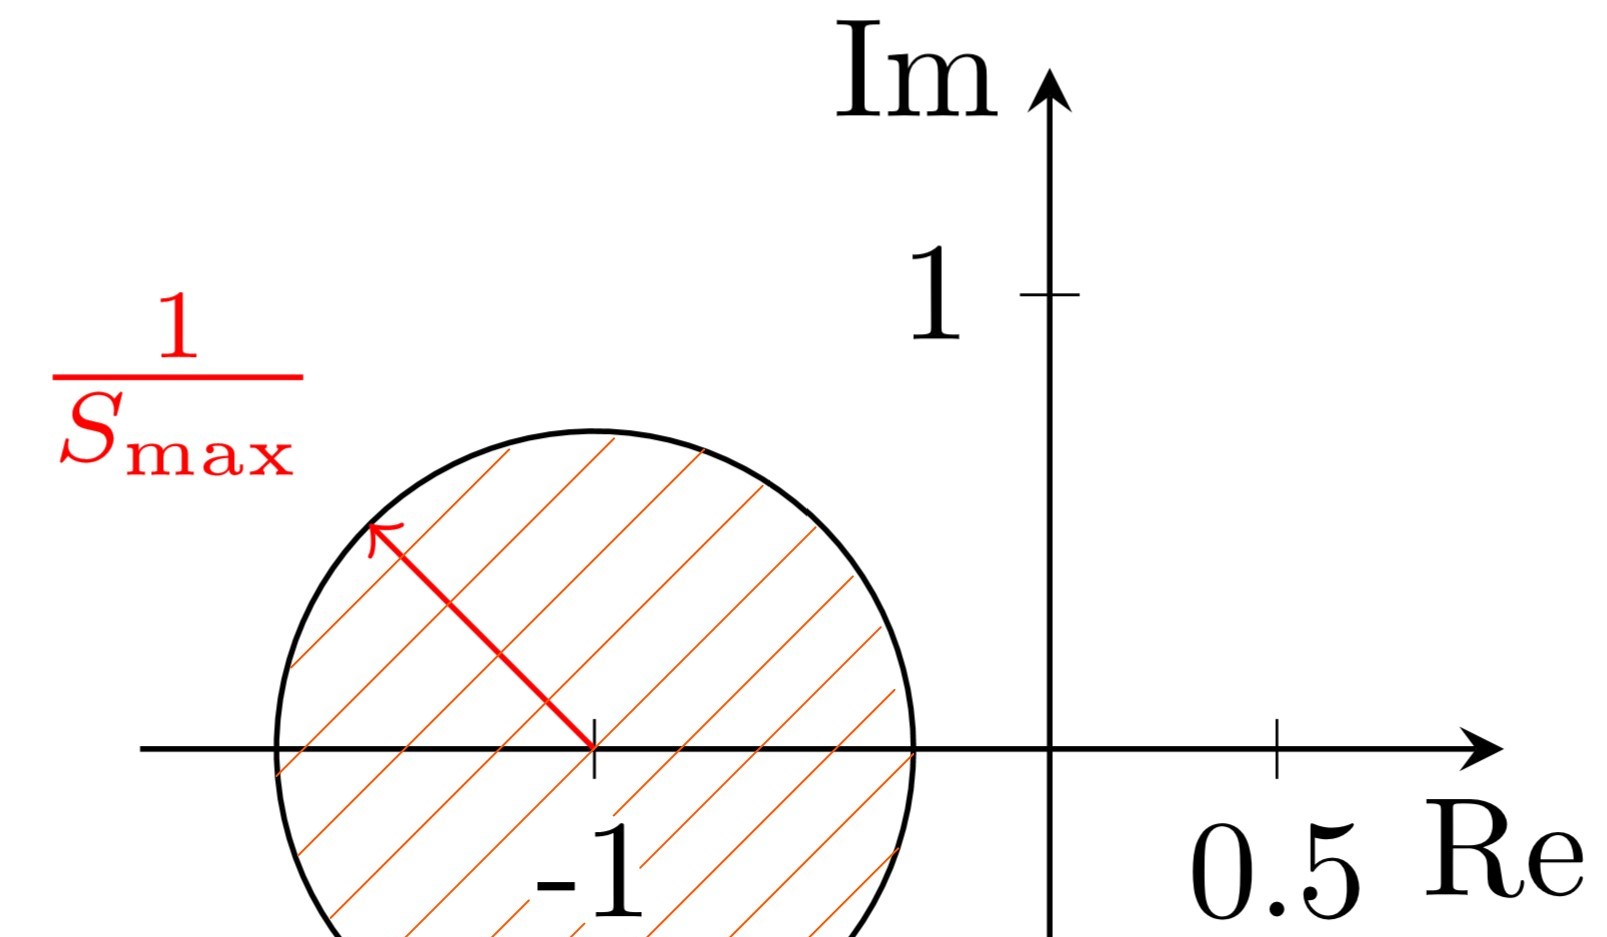
\includegraphics[width = 0.6\linewidth]{images/08/Spezifikation_im_FB.jpg}
            \end{center}
         $L(j\omega)$ darf nicht in einem in -1 zentrierten Kreis mit Radius $\frac{1}{S_{max}}$ eintreten.
         
            \textbf{Die geometrische Interpretation von}
            \[L(j\omega)\notin\Bigg\{\Bigg|\frac{T_{max}^2}{T_{max}^2-1}+z\Bigg| \leq \frac{T_{max}}{T^2_{max}-1}\Bigg|z\in\mathbb{C}\Bigg\}\]
            \begin{center}
                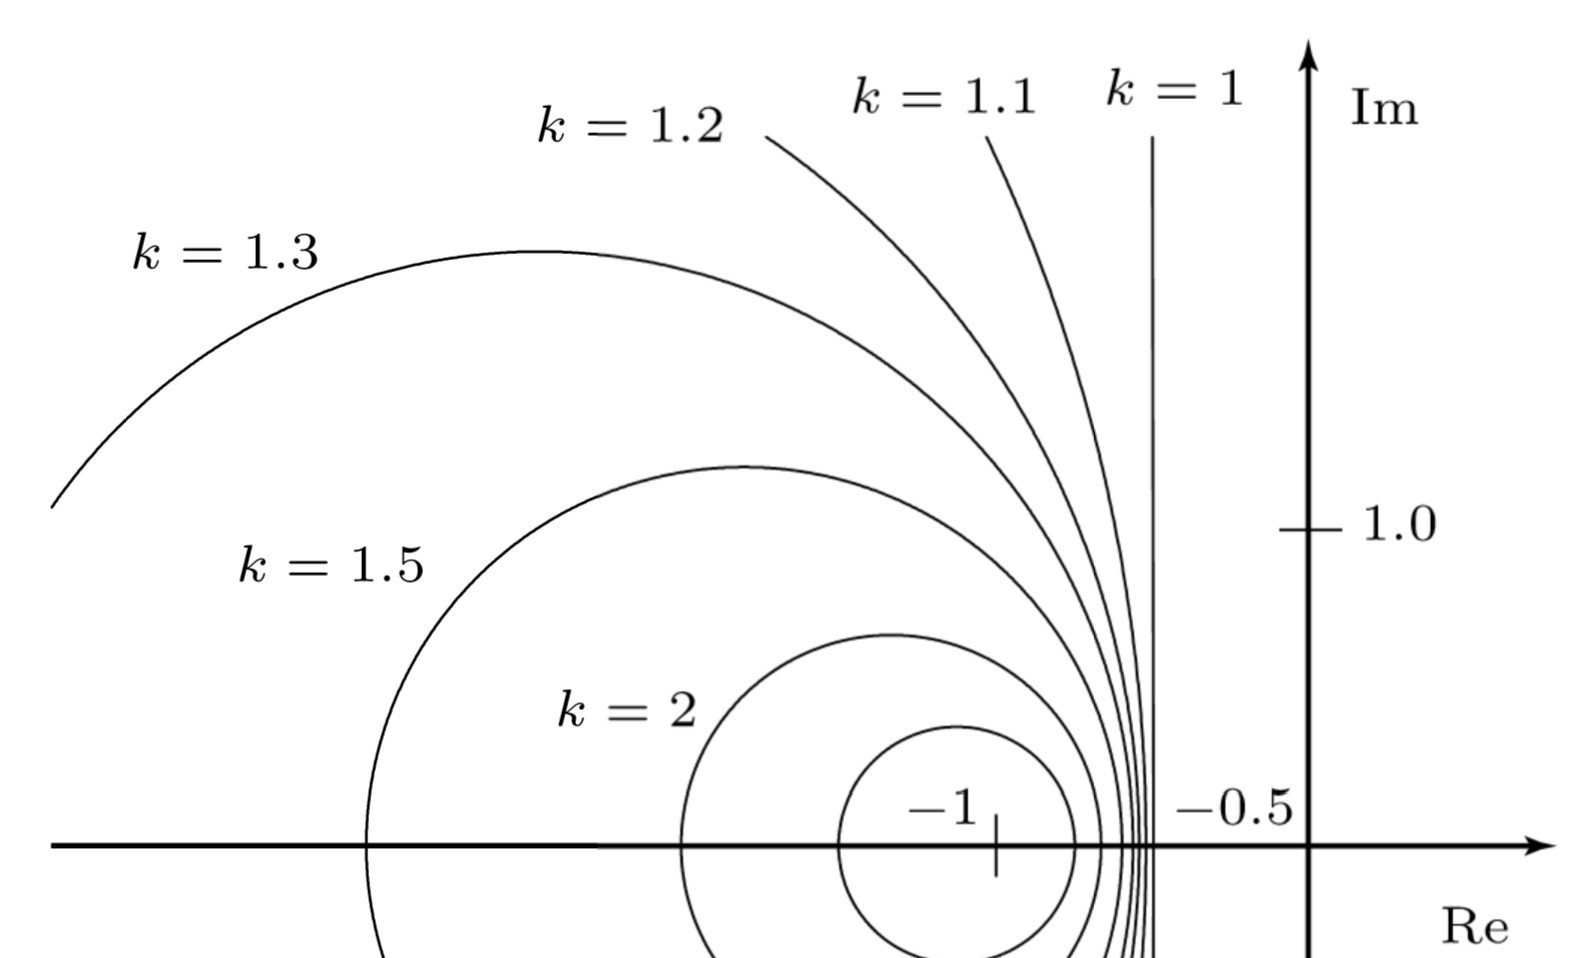
\includegraphics[width = 0.8\linewidth]{images/08/Spezifikation_im_FB2.jpg}
            \end{center}
            $L(j\omega)$ darf nicht in einem in $\frac{-T^2_{max}}{T^2_{max}-1}$ zentrierten Kreis mit Radius $\frac{T_{max}}{T^2_{max}-1}$ eintreten.

\vfill\null\columnbreak
\section{Reglerauslegung}
    \subsection{PID-Regler}
        \begin{center}
           \begin{tabular}{|c|c|c|}
              \textbf{Proportionalregler}  & (\textbf{P}-Term) & $e(t)$ \\
               \textbf{Integralregler} & (\textbf{I}-Term) & $\frac{1}{T_i}\cdot\int_0^t e(\tau)d\tau$ \\
               \textbf{Derivative-Term} & (\textbf{D}-Term) & $T_d\cdot\frac{d}{dt}e(t)$
           \end{tabular}
        \end{center}
        Der \textbf{I}-Term wird betragsmässig grösser, je länger ein einseitger Fehler (z:B. $e(t) > 0$) vorhanden ist. 
        Der \textbf{D}-Term wirkt auf schnelle Änderungen im Fehlersignal. Ein Nachteil des D-Terms ist, dass er Rauschen auf dem Fehlersignal $e(t)$ verstärkt.
          
        Eine Transformation in den Frequenzbereich ergibt
        \begin{center}
        \begin{tabular}{|c|c|c|}
          \textbf{Proportionalregler}  & (\textbf{P}-Term) & $1$ \\
           \textbf{Integralregler} & (\textbf{I}-Term) & $\frac{1}{T_i\cdot s} $\\
           \textbf{Derivative-Term} & (\textbf{D}-Term) & $T_d\cdot s$
        \end{tabular}
        \end{center}
        
        Im Zeitbereich sieht ein PID-Regler folgendermassen aus.
        
       \[U_\textrm{PID}(t) = k_p\cdot\Bigg(e(t)+ \frac{1}{T_i}\cdot\int_0^t e(\tau)d\tau +T_d\cdot\frac{d}{dt}e(t)\Bigg)\]
       
       in den Frequenzbereich transformiert ergibt sich folgendes:
       \[C_\textrm{PID}(s) = k_p\cdot\Bigg(1+\frac{1}{T_i\cdot s} + T_d\cdot s\Bigg)=\frac{U(s)}{E(s)}
       \]
       Da der D-Term sehr empfindlich auf Rauschen ist werden hohe Frequenzen ganz einfach unterdrückt, indem man eine hochfrequente doppelte Nullstelle an den Regler hängt. Sogenannte \textbf{roll-off} Term $\rightarrow \frac{1}{(\tau\cdot s+1)^2}$.
       \[C_\textrm{PID}(s) = k_p \cdot\overbrace{\Bigg(\underbrace{\frac{T_d\cdot T_i\cdot s^2+T_i\cdot s+1}{T_i\cdot s}}_\textrm{nicht kausal}\Bigg)\cdot  \frac{1}{(\tau\cdot s+1)^2}}^\textrm{kausal}\]
       
       Ohne den roll-off Term wäre die Übertragungsfunktion $\frac{U(s)}{E(s)}$ nicht kausal und entsprechen nicht praktisch realisierbar. Um $u(t)$ ohne roll-off zu berechnen, bräuchte man Zukunftswerte des Fehlersignals $e(t)$.\\\\
        \textbf{PID-Regler als Standardform im Frequenzbereich}
        \begin{center}
            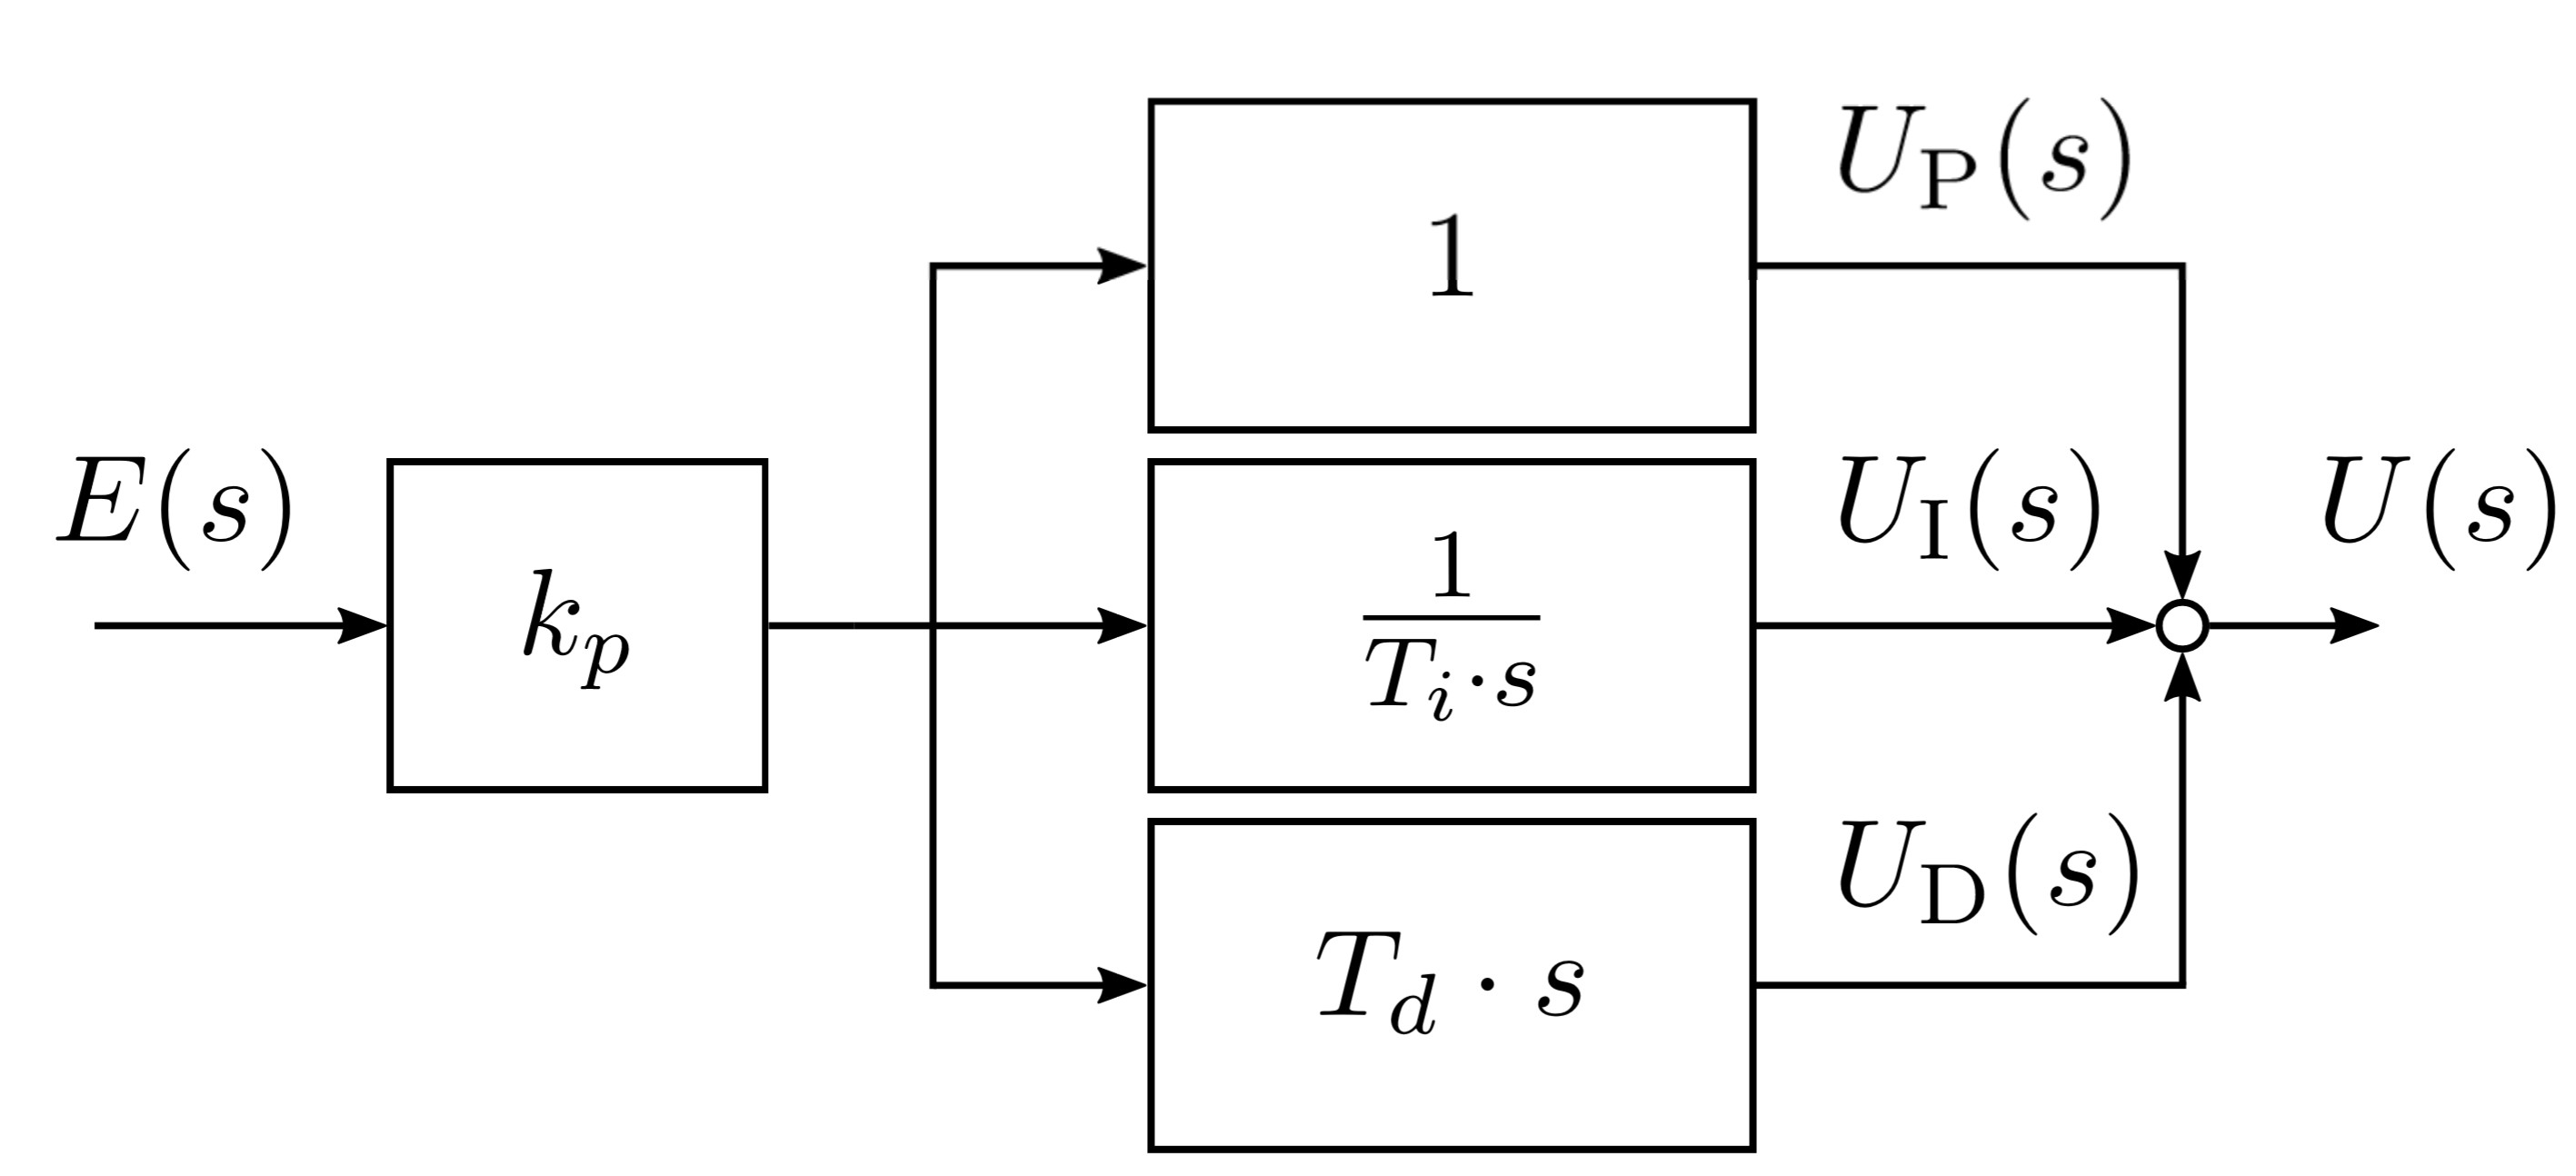
\includegraphics[width = 0.6\linewidth]{images/09/PID-regler.jpg}
        \end{center}
        
        \textbf{Pro Term ein Freiheitsgrad:} Dh. mit einem P Regler kann nur die Durchtrittsfrequenz \textit{ODER} die Phasenreserve eines Systems individuell verändert werden. Um beide Terme beinflussen zu können braucht man mehr Freiheitsgrade!
        
    \subsubsection{P-Term}
        \[
        u_\textrm{P}(t)= k_p\cdot e(t), \hspace{3mm} U_\textrm{P}(s) = k_p\cdot E(s)
        \]
        Der P-Term reagiert auf momentanen Wert des Fehlers $e(t)$. Die Stärke der Reaktion ist proportional zur Grösse des momentanen Fehlers.
    \subsubsection{I-Term}
        \[
        u_\textrm{I}(t) = \frac{k_p}{T_i}\cdot\int_0^te(\tau)d\tau, \hspace{3mm} U_\textrm{I}(s)=\frac{k_p}{T_i}\cdot\frac{1}{s}\cdot E(s)
        \]
        
        Der I-Term reagiert zum Zeitpunkt $t$ proportional auf den kumulierten Fehler, für $t\in[0,t]$. Falls ein statischer Nachlauffehler vorhanden ist, wird dieser aufintegriert, und der Reglerausgang wird immer grösser, bis kein Fehler mehr vorhanden ist. Ein Nachteil des Integrators ist, dass der Reglerausgang theoretisch beliebig gross werden kann.
        
        I-Terme führen immer zu einem \textbf{Phasenverlust}.
        
        \subsubsection{D-Term}
        \[u_\textrm{D}(t) = k_p\cdot T_d \cdot \frac{d}{dt}e(t),\hspace{3mm} U_\textrm{D}(s) = k_p\cdot T_d\cdot s\cdot E(s)\]
        
        Der D-Term wirkt antizipierend, er reagiert zum Zeitpunkt $t$ auf die momentane Änderungsrate des Fehlers. Der D-Term wirkt wie ein Dämpfer gegen ein schnelles Erhöhen oder Verringern des Fehlers. Eine starke Änderung im Fehler resultiert in einem erhöhten Reglerausgang. Falls die Änderung zu stark ist, kann der gewünschte Reglerausgang grösser als der grösst mögliche Eingang eines Systems werden. 
        
        D-Terme führen immer zu einem \textbf{Phasenanstieg}.
        \subsubsection{Bodediagramm eines PID-Reglers mit roll-off}
            \begin{center}
                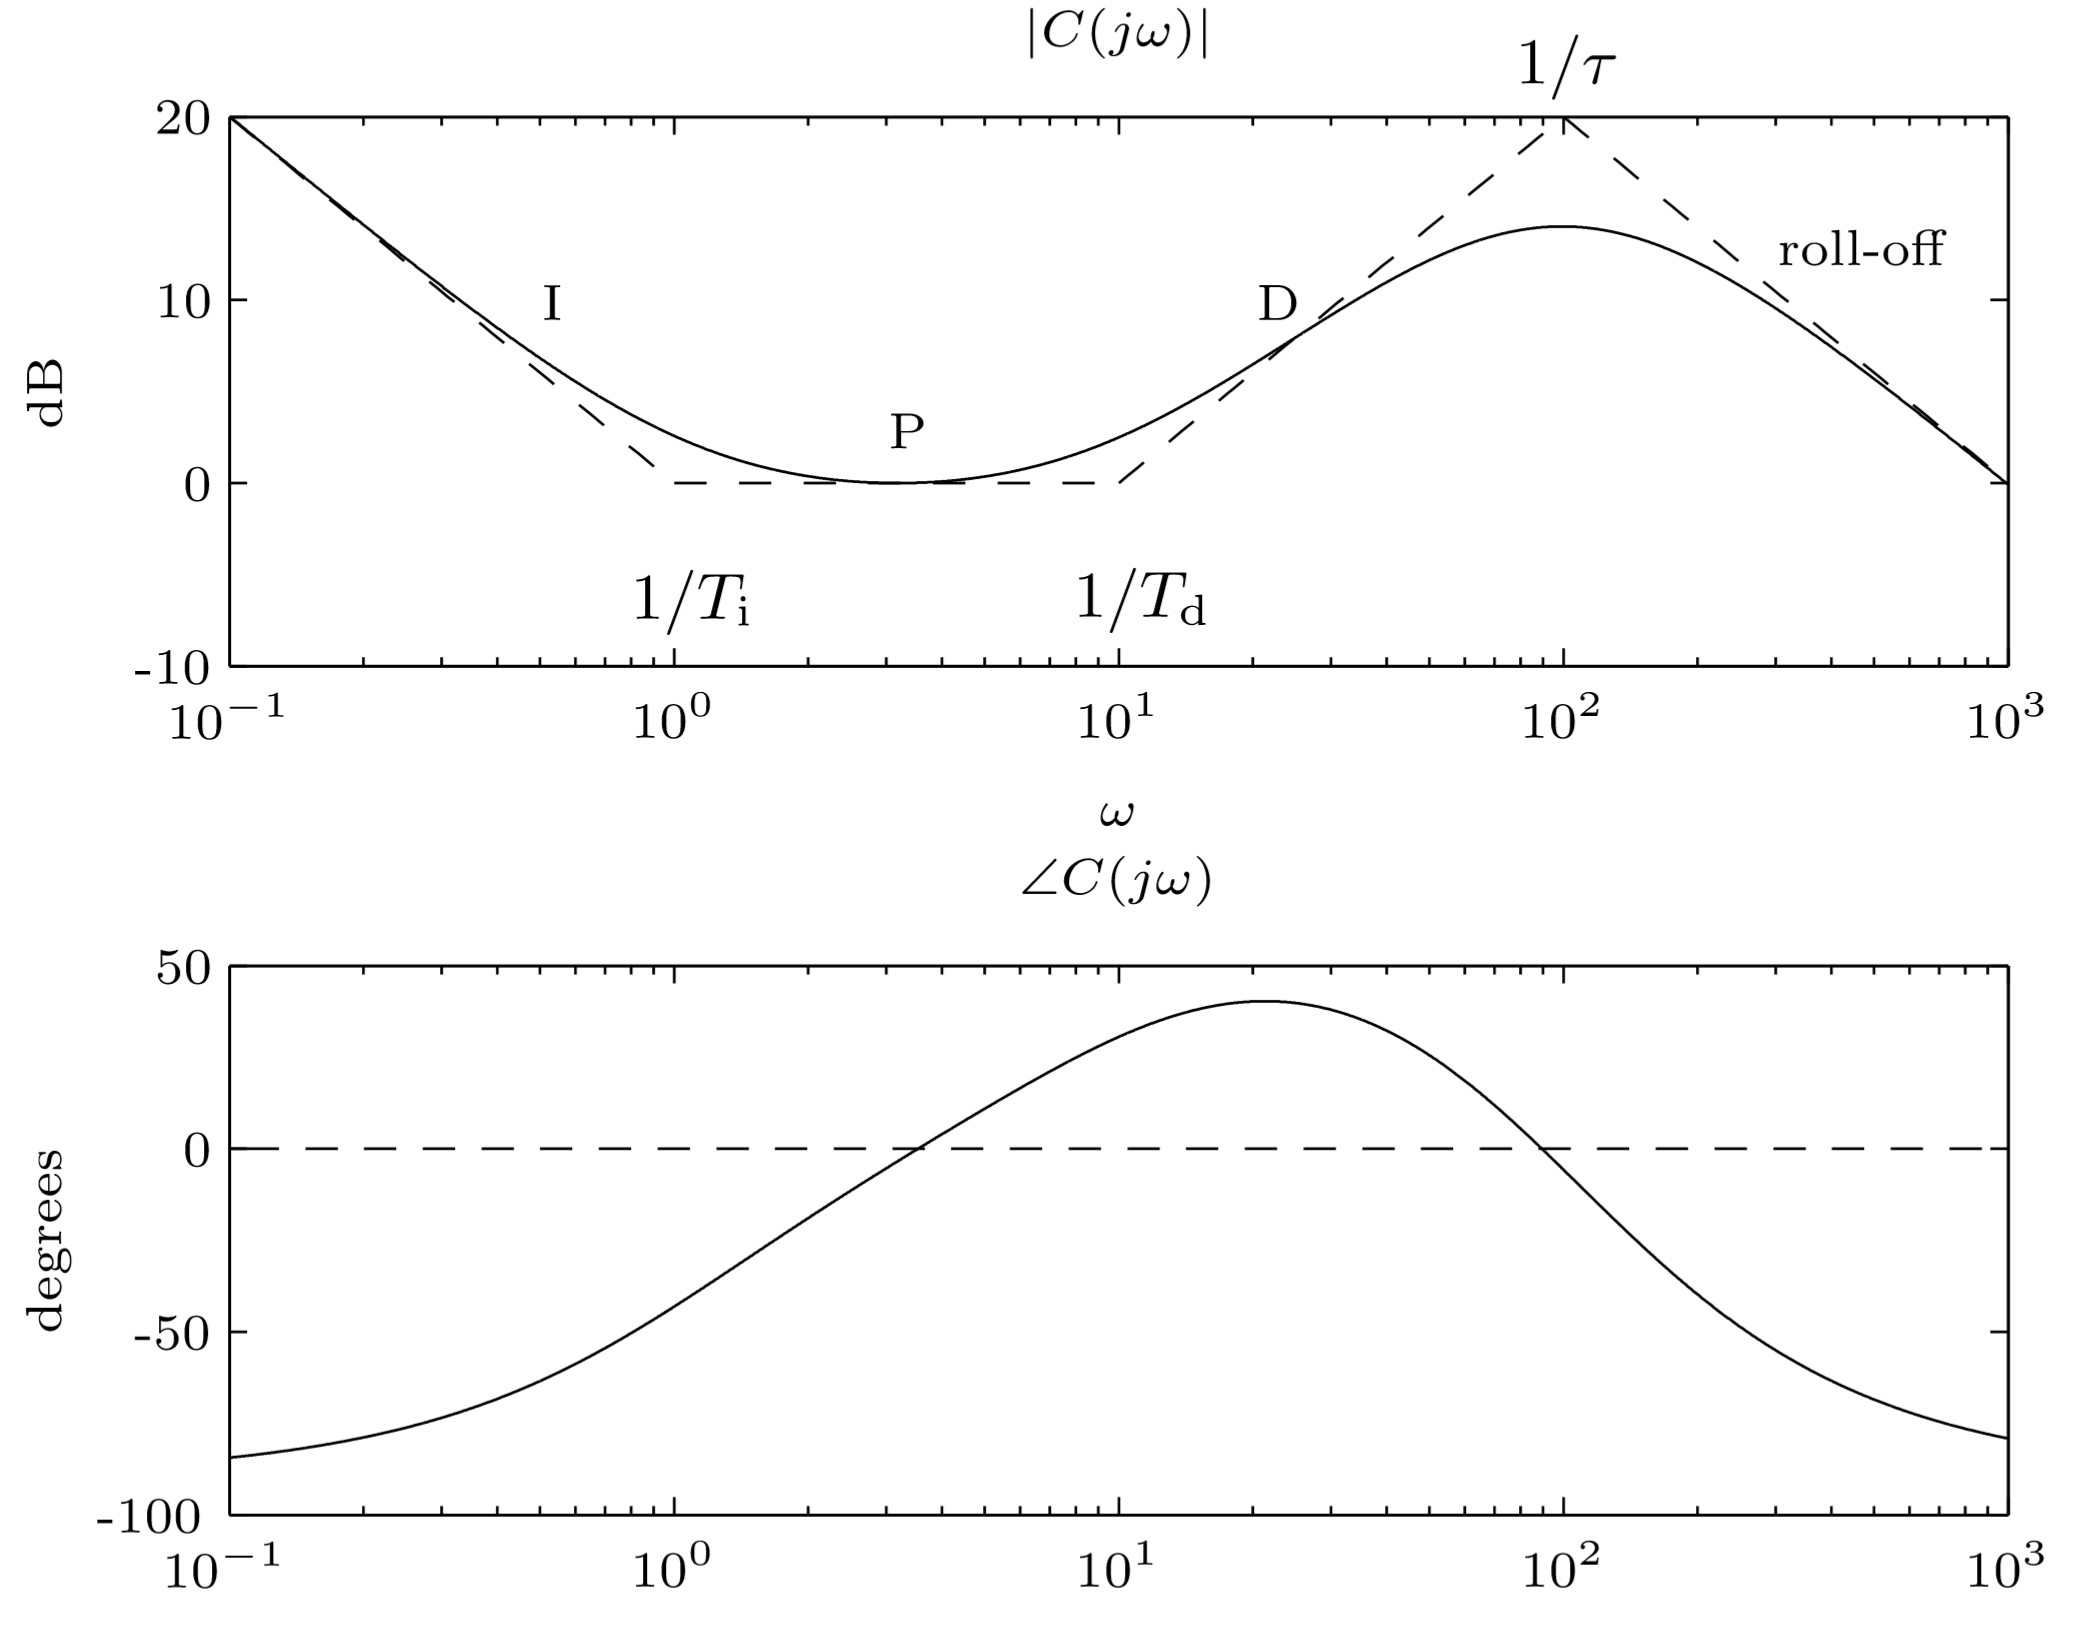
\includegraphics[width=\linewidth]{images/09/Bodediagramm_roll-off.jpg}
            \end{center}
        
        \subsubsection{Bsp}
            \textbf{Regelung eines Systems 2. Ordnung}
            \begin{center}
                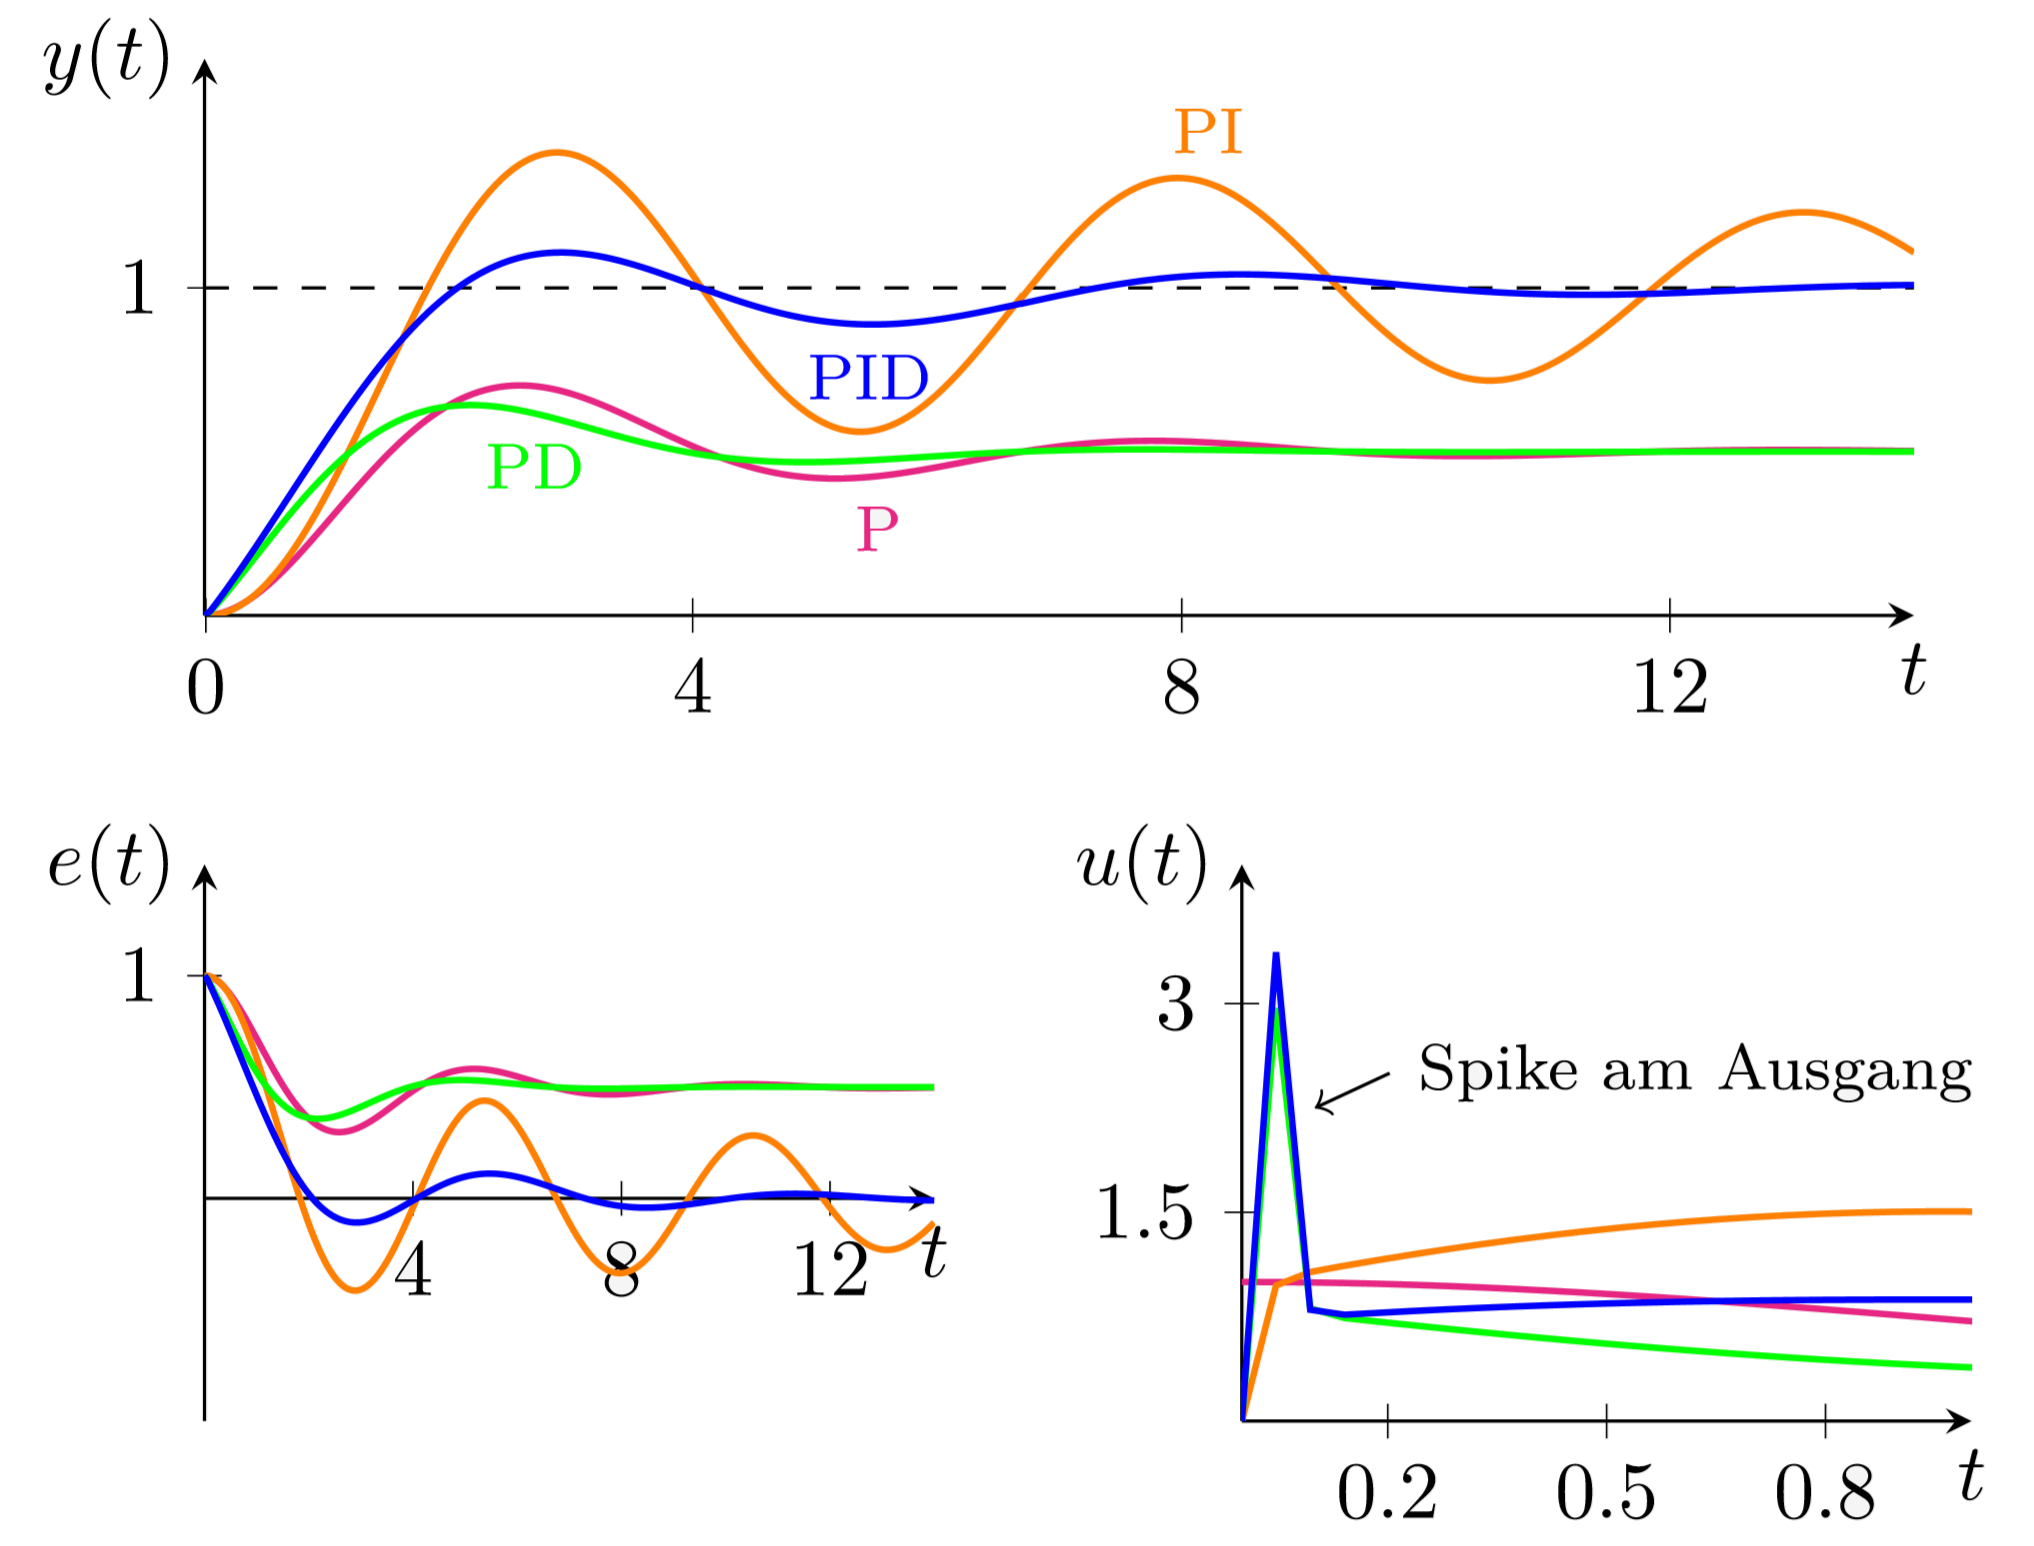
\includegraphics[width =\linewidth]{images/09/Bsp_PID.png}
            \end{center}
            Es ist ersichtlich, dass ein statischer Fehler durch den Integrator eliminiert werden kann. Der D-Term ermöglicht es, schneller auf die Fehleränderung zu reagieren, jedoch wird dadurch der Reglerausgang auch grösser.
\vfill\null\columnbreak            
        \subsubsection{Bsp}
            \textbf{Bode and Nyquist Plots of mass-oscillator example}
            \[P(s)=\frac{1}{(s+1)^2}\]
            \begin{center}
                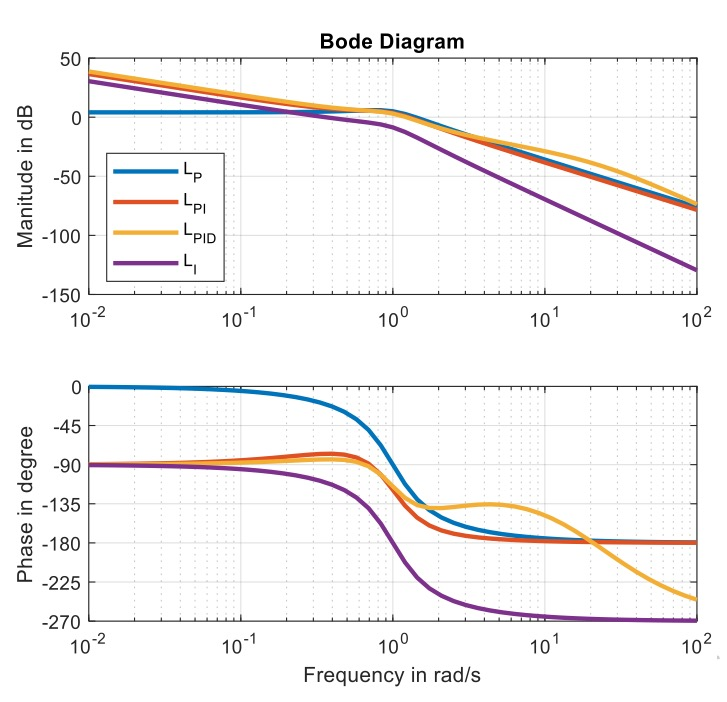
\includegraphics[width = 0.9\linewidth]{09/PID_Bode.jpg}
                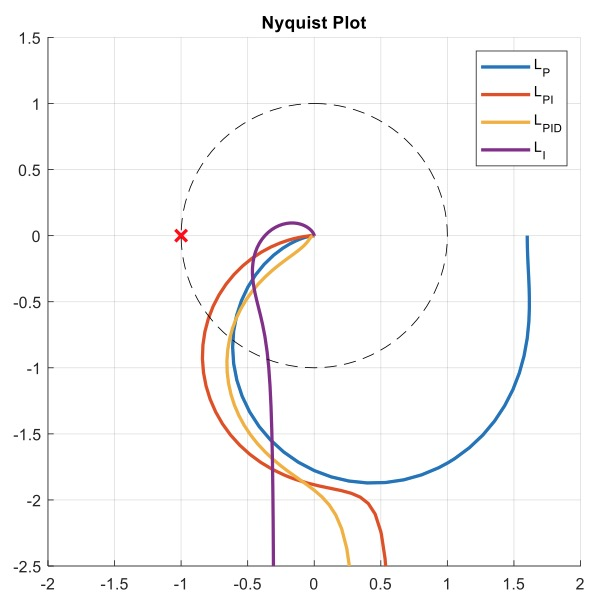
\includegraphics[width = 0.9\linewidth]{09/PID_Nyquist.jpg}
            \end{center}
    \subsection{PID-Regler Parameter Tuning nach Ziegler Nichols}
        Die Parameter $k_p,T_i$ und $T_d$ können durch extensives Testen des Systems bestimmt werden. Ein anderer Ansatz ist, der von Ziegler-Nichols. Hier geht man davon aus, dass das System $P(s)$ ein System erster Ordnung, mit zusätzlicher relativ kleiner Totzeit ist 
        \[P(s) \approx \frac{k}{\tau\cdot s + 1}\cdot e^{-T\cdot s},\hspace{3mm} \textrm{wobei:} \frac{T}{T+\tau}\overset{!}{<} 0.3\]
        Zur Bestimmung der Ziegler-Nichols Parameter startet man mit einem reinen P-Regler und erhöht die Verstärkung $k_p$ soweit, bis der geschlossene Regelkreis grenzstabil wird bei der Verstärkung $k_p^*$ (Pole von $T(s)$ auf der imaginären Achse). Falls die Modellannahme ungefähr stimmt, oszilliert das grenzstabile System bei $k_p^*$ mit einer Periode von $T^*$. Man kann diese Parameter des grenzstabilen System in folgende Tabellen einsetzen um Reglerparamter für verschiedene PID Kombinationen zu erhalten.
        \\$\omega^*$: Frequenz, bei der Phase $= -\pi$.
        \[\boxed{|k_p^* \cdot P(j\omega^*)| \overset{!}{=} 1} \hspace{3mm}
        \boxed{\angle k_p^* \cdot P(j\omega^*)\overset{!}{=}-\pi} \hspace{3mm}
        \boxed{T^* =\frac{2\pi}{\omega^*}}\]
        \begin{center}
        {\renewcommand{\arraystretch}{1.5}
            \begin{tabular}{l r r r}
            Regler & $k_p$ & $T_i$ & $T_d$ \\
                 \hline
                P & $0.5\cdot k_p^*$ & $\infty \cdot T^*$ & $0 \cdot T^*$ \\
                PI & $0.45\cdot k_p^*$ & $0.85\cdot T^*$ & $0 \cdot T^*$\\
                PD & $0.55 \cdot k_p^* $& $\infty \cdot T^*$ &  $0.15\cdot T^*$\\
                PID & $0.6\cdot k_p^*$ & $0.5 \cdot T^*$ & $0.125 \cdot T^*$\\
            \end{tabular}}
        \end{center}
    
        \subsubsection{Bsp}
            Gegeben sei folgendes System:  
            \[P(s) = \frac{1}{s(s+1)(s+2)}\]
            man soll mit Ziegler /Nichols ein Regler auslegen.
            Zur Bestimmung der kritischen Verstärkung $k_p^*$ und der kritischen Frequenz $\omega^*$ können die folgenden Beziehungen verwendet werden:
            \[k_p^* \cdot P(j\omega^*) \overset{!}{=} -1+0j\]
            Es folgt somit
            \begin{align*}
            \frac{k_p^*}{-j(\omega^*)^3-3(\omega^*)^2+2j\omega^*} &= -1\\
            k_p^* &= -(-3(\omega^*)^2 - j((\omega^*)^3-2\omega^*))\\
            k_p^* &= 3(\omega^*)^2+j((\omega^*)^3-2\omega^*)
            \end{align*}
            
            Aus dem Vergleich des Imaginärteils findet man 
            \[
            (\omega^*)^3-2\omega^* = \omega^* \cdot((\omega^*)^2-2) = 0\]
            Da wir nur an positiven realen Frequenzen ($k_p^* \in \mathbb{R}$) interessiert sind, folgt $\omega^*=\sqrt{2}$ Aus dem Vergleich der Realteilen folgt
            \[
            k_p^* = 3(\omega^*)^2 = 6
            \]
    \subsection{Iterative Loop Shaping}
        Ein System, das mit einem PID-Regler ausgelegt wird, erfüllt unter Umständen nicht alle Designspezifikationen. Um gewisse Frequenzbänder nach Wunsch abzuändern, kann man einen beliebigen Regler zum Beispiel mit Lead-/Lag- Elemente erweitern oder einen Regler von Grund auf neu
        erstellen. 
    \subsection{Lead-Lag Elemente 1. Ordnung}
        der Term 'Lead-Lag' bezeichnet zwei Arten von Systemen mit gleicher Struktur und den zwei Parametern $\alpha$ und $T$:
        \[
        C(s) = \frac{T\cdot s + 1}{\alpha \cdot T \cdot s + 1}, \hspace{3mm} \alpha,T\in \mathbb{R}_+
        \]
        Der Wert von $\alpha$ definiert ob es sich um ein Lead- oder ein Lag- Element handelt: 
        \begin{align*}
            0 &< \alpha < 1 & \Leftrightarrow \textrm{Lead-Element} \\
            1 &< \alpha     & \Leftrightarrow \textrm{Lag- Element}
        \end{align*}
        Die Parameter $\alpha$ und $T$ werden gezielt gewählt, sodass bei der Frequenz $\hat{\omega}$ eine maximale Phasenänderung von $\hat{\varphi}$ vorliegt:
        \[\alpha = \Big(\sqrt{\tan^2(\hat{\varphi}+1}-\tan(\hat{\varphi})\Big)^2, \hspace{3mm} T = \frac{1}{\hat{\omega}\cdot\sqrt{\alpha }}\]
        \begin{center}
            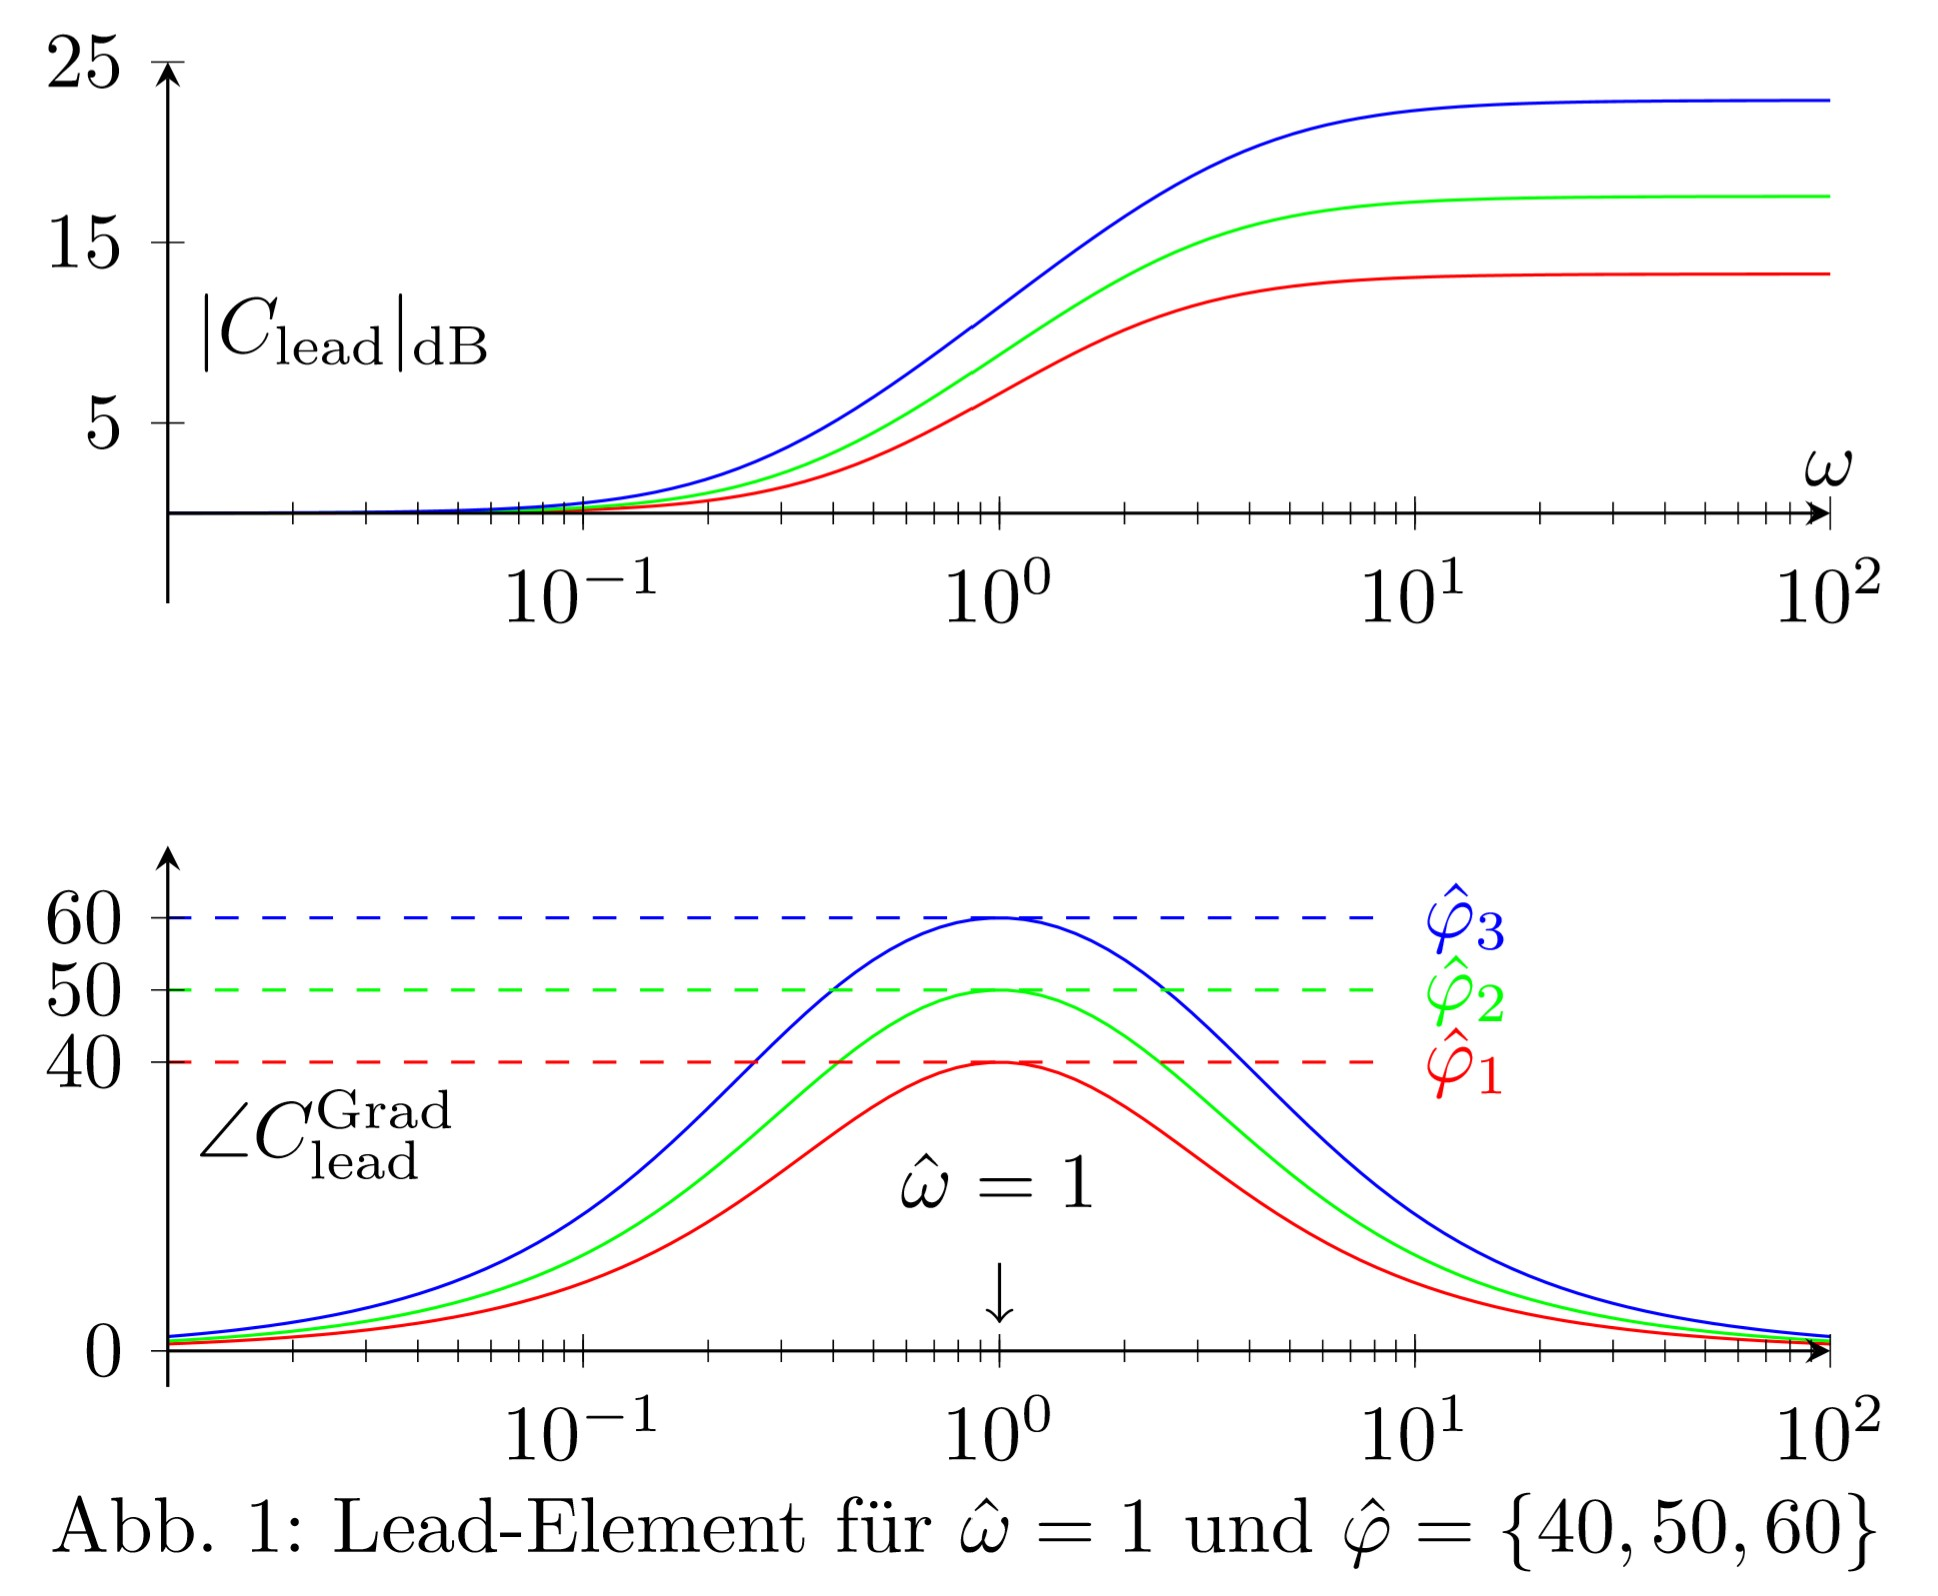
\includegraphics[width = 0.85\linewidth]{images/09/Lead_Lag_pos.jpg}
            \includegraphics[width = 0.8\linewidth]{images/09/Lead_Lag_neg.jpg}
        \end{center}
        Ein Lag- Element mit $-\hat{\varphi}$ entspricht einer Spiegelung des Magnituden und Phasendiagramms des Lead-Elements mit $\hat{\varphi}$.
    \subsection{Lead-Lag Elemente 2. Ordnung}
        Die Verwendung eines Elements 1. Ordnung beeinflusst Frequenzen in der grösseren Umgebung von $\hat{\omega}$. Die Idee eines Elements 2. Ordnung ist, dass der gewünschte Effekt an einer bestimmten Frequenz besser isoliert ist. Die Struktur erfordert die Parameter $\kappa, \epsilon,$ und $\omega_0$
        \[
        C(s) = k\cdot\frac{s^2 +2\cdot\kappa\cdot\epsilon\cdot(1-\epsilon)\cdot\omega_0\cdot s+(1-\epsilon)^2\cdot\omega_0^2}{s^2+2\cdot\kappa\cdot\epsilon\cdot(1+\epsilon)\cdot\omega_0\cdot s+(1+\epsilon)^2\cdot\omega_0^2}\]
        
        Zusätzlich zur Wahl der mittleren Frequenz $\hat{\omega}$ und der maximalen Phasenverschiebung $\hat{\varphi}$ kann man nun zusätzlich die Breite des Frequenzbands durch den Parameter $\epsilon$ wählen:
        \[ k = \frac{(1+\epsilon)^2}{(1-\epsilon)^2},\hspace{3mm} \kappa=\frac{\cot(\hat{\varphi}/2)}{\sqrt{1-\epsilon^2}},\hspace{3mm} \omega_0 = \frac{\hat{\omega}}{\sqrt{1-\epsilon^2}}\]
        \begin{center}
            \includegraphics[width = 0.8\linewidth]{images/09/Lead_Lag_2.jpg}
        \end{center}
            
    \subsection{Inversion der Regelstrecke}
        Wenn die Regelstrecke $P(s) = \frac{n_p(s)}{d_p(s)}$ mit relativem Grad $r$ asymptotisch stabil ist und nur minimalphasige Nullstellen enthält, kann ein Regler $C(s)$gewählt werden, der die Dynamik der Regelstrecke exakt kompensiert und gleichzeitig in einer gewünschten Übertragungsfunktion $L(s)$ des offenen Regelkreises resultiert:
        \begin{align*}
            L(s) &= P(s)\cdot \underbrace{P(s)^{-1}\cdot\overbrace{\frac{1}{T_i\cdot s}\cdot\frac{1}{(\tau\cdot s + 1)^{r-1}}}}^{\textrm{desired }L(s)}_{C(s)}\\
            \Rightarrow C(s) &= P(s)^{-1}\cdot\frac{1}{T_i\cdot s}\cdot\frac{1}{(\tau\cdot s + 1)^{r-1}}\\
            C(s) &= \frac{d_p(s)}{n_p(s)}\cdot\frac{1}{T_i\cdot s}\cdot\frac{1}{(\tau\cdot s + 1)^{r-1}}
            \end{align*}
            
        Der Regler invertiert die Dynamik der Regelstrecke, und somit haben die Pole und Nullstellen von $P(s)$ keinen Einfluss auf die Übertragungsfunktion des offenen Regelkreises $L(s$. Die übrigen Elemente von C(s) stellen sicher, dass die gewünschte Übertragungsfunktion $L(s)$ des offenen Regelkreises resultiert:
        \[L(s) = \frac{1}{T_i\cdot s}\cdot \frac{1}{(\tau\cdot s + 1)^{r-1}}\]
        Mit der Verstärkung $T_i = \omega_c^{-1}$ kann die gewünschte Durchtrittsfrequenz $\omega_c$ eingestellt werden. Zusätzlich wählen wir $\tau < T_i$ und $\omega_c < \omega_2$.
        
    \subsection{Bsp maximale Totzeit}
        Für welche maximale Totzeit $e^{-\tau s}$ ist der geschlossene Regelkreis (mit $C(s)=k_p=1$ noch stabil?
        \begin{enumerate}
            \item $\omega_c$ bei dem $|\Sigma(S)|=0 dB$ aus Bode auslesen.
            \item Phasenreserve $\varphi$ in radian berechnen
            \item $\tau_{max}=\frac{\varphi}{\omega_c}$
        \end{enumerate}

\end{multicols*}

\includepdf[pages=-, nup=2x1, delta= -10mm -10mm, addtotoc={1, section, 1, {Appendix A}, appendix}]{resources/Guzzella_RT1_Appendix_A.pdf}

\end{document}